\documentclass[11pt,a4paper]{report}

\usepackage{fontspec}
  \setmainfont{TeX Gyre Pagella}

\usepackage{amsmath}
  \DeclareMathOperator*{\argmax}{arg\,max}
\usepackage{amsthm}
  \newtheorem*{theorem}{Theorem}
\usepackage{amssymb}
\usepackage[backend=biber,style=alphabetic,citestyle=authoryear]{biblatex}
  \addbibresource{references.bib}
\usepackage{booktabs}
\usepackage{commath}
\usepackage{csquotes}
\usepackage{graphicx}
  \graphicspath{{figs/}}
\usepackage[hidelinks,pdfusetitle]{hyperref}
\usepackage{mathtools}
\usepackage{mdframed}
\usepackage{multirow}
\usepackage{siunitx}
  \sisetup{detect-all,binary-units}
\usepackage{subcaption}
\usepackage{todonotes}

\title{Determining Confidence Measures on Fundamental Frequency Estimations}
\author{Boyuan Deng}
\date{July 2016}

\begin{document}

\maketitle

\thispagestyle{empty}

Supervised by:

\textit{Denis Jouvet}, Inria Nancy-Grand Est, France

\textit{Ingmar Steiner}, Saarland University, Germany

\bigskip

Co-supervised by:

\textit{Yves Laprie}, CNRS, France

\bigskip

Work done at Inria Nancy-Grand Est with the Inria MULTISPEECH team.

\medskip

Submitted to Saarland University, University of Lorraine and Erasmus Mundus LCT Consortium.

% \todo{fancy minipages and icons, also more info}

\vfill

\noindent \textbf{Eidesstattliche Erklärung}

\smallskip

\textit{Hiermit erkläre ich, dass ich die vorliegende Arbeit selbstständig verfasst und keine anderen als die angegebenen Quellen und Hilfsmittel verwendet habe.}

\medskip

\noindent \textbf{Declaration}

\smallskip

\textit{I hereby confirm that the thesis presented here is my own work, with all assistance acknowledged.}

\bigskip

\noindent Nancy, France

\bigskip

\noindent Date \hspace{3cm} Signature

\newpage

\thispagestyle{empty}

\section*{Acknowledgements}

I would like to thank my supervisors for their guidance and help during the research process, and Aghilas Sini for maintaining the \texttt{JSnoori} toolkit.

Furthermore, I would like to thank staff at LORIA/Inria Nancy-Grand Est for hosting my stay.

\bigskip

Experiments presented in this article were carried out using the
Grid'5000 testbed, supported by a scientific interest group hosted by
Inria and including CNRS, RENATER and several Universities as well as
other organizations (see \url{https://www.grid5000.fr}).


\begin{abstract}
Fundamental frequency estimation acts as the basis of many applications related to speech or music, such as speaker recognition, development of speech synthesis voices and music information retrieval.
Various algorithms working in the time or frequency domain have been developed in the past and work quite well on good-quality signals.
They become more error prone on lower-quality signals but none of them indicate how reliable the estimation results are, which is a crucial metric if the overall system makes decisions based on probabilities or multiple estimation algorithms are combined using ensemble methods.

In our work, we tackle this problem by developing and evaluating confidence measures based on machine learning approaches for several existing fundamental frequency estimation algorithms.
Such confidence measure can be seen as the probability of the estimation result to be correct.
Sophisticated neural network architectures, including long short-term memory networks (LSTM), are chosen for the construction of these measures.
And numerous features computed on the signals and generated during estimations are used as input.

Besides confidence measures, our work also illustrates some empirical analyses on the robustness of existing fundamental frequency estimation algorithms.
Data from an audio corpus is artificially distorted in a quantitatively controlled way, by modifying signal levels or adding certain types of noise at given signal-to-noise ratios, etc.
Changes in error rates as well as the different error types (deviation or error in voiced/unvoiced decisions) are visualized and the underlying causes are analyzed in detail.
The conclusions drawn may help guide the choice of fundamental frequency estimation algorithms depending on situations and needs.
\end{abstract}

\tableofcontents

\listoffigures
\listoftables

\chapter{Introduction}

The two keywords of our work are \enquote{fundamental frequency} and \enquote{confidence measure}.

\bigskip

Fundamental frequency, defined as the lowest frequency of a periodic waveform, is a vital measure in audio processing.
It can reflect a speaker's gender, emotional state, etc.\ in speech processing.
And in any kind of content-based music processing, such as genre analysis, music retrieval and recommendation, etc.\, fundamental frequency is the bridge between audio and musical note representations.
Applications in these fields explicitly conduct fundamental frequency estimations in early stages or produce intermediate representations closely related to fundamental frequency, especially by using neural network methods.

Real-life audio signals won't be perfectly periodic.
Taking this into account, various fundamental frequency estimation algorithms working in the time domain, frequency domain, or both have been developed over the past decades.
There is no single ideal estimation algorithm until now because of the variety of aperiodicity.

The original literature of existing fundamental frequency estimation algorithms usually reports average accuracies on clean signals, i.e.\, naturally generated sounds recorded by professional equipment.
The error rates must be rising when the clean signals are distorted, but to what extent? Will there be differences between various algorithms' performance and what are the causes? We conduct a series of empirical analyses in \autoref{emp-aly} to uncover these.

\bigskip

Then we move attention from average accuracies on a large audio corpus to the correctness of individual results.
This is formalized as confidence measure, a concept widely used in statistics and computer science.

As far as we know, none of the existing fundamental frequency estimation algorithms provide confidence measures along with estimation results.
It will be a meaningful piece of work to construct such confidence measures, after which better results can be obtained by combining existing estimation algorithms using ensemble methods.
They also enable us to integrate the algorithms into bigger systems.

We start from an important theorem linking confidence measures and neural network classifiers, then develop and evaluate confidence measures based on sophisticated neural network methods, which is shown in the latter part of this thesis.

\chapter{Background and Related Works}

\section{Fundamental frequency estimation algorithms}

We focus on three widely used fundamental frequency estimation algorithms, namely Martin's algorithm \parencite{martin1982comparison}, SWIPE \parencite{camacho2007swipe} and YIN \parencite{de2002yin}.
They are implemented in the \texttt{JSnoori} toolkit\footnote{\url{http://jsnoori.loria.fr/}}.

Fundamental frequency estimations are conducted \enquote{locally} at given time offsets using the information within a very short context window.
F0 values change rapidly in audio files (most obvious for music) so the results are valid locally only, too.

The implementations iterate through audio files, output estimated fundamental frequencies at time indices where the user has interest (usually defined through starting point and interval).
The results can be visualized by software programs such as Wavesurfer\footnote{\url{http://www.speech.kth.se/wavesurfer/}} \parencite{sjolander2000wavesurfer}.

\begin{figure}[htbp]
  \centering
  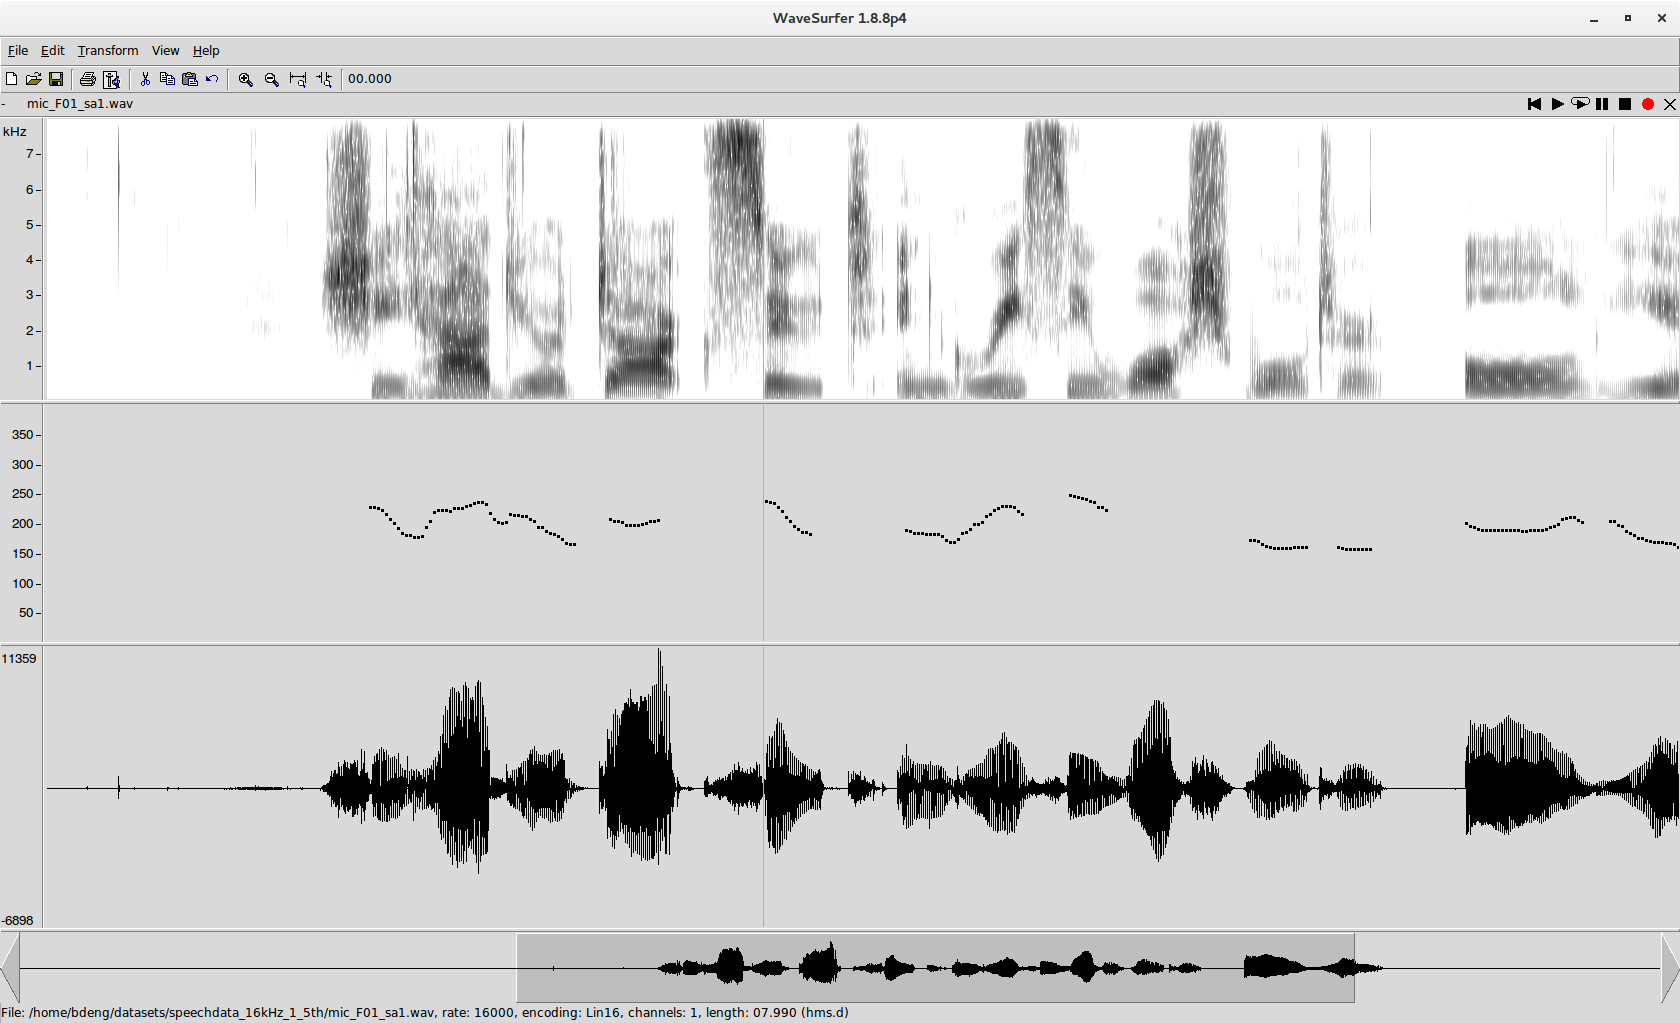
\includegraphics[width=\textwidth]{wavesurfer.png}
  \caption{Spectrogram, plot of reference F0 values, and waveform shown in Wavesurfer.} \label{fig:wavesurfer}
\end{figure}

\subsection{Common problems in fundamental frequency estimation}

\begin{itemize}
  \item Results doubling or halving with respect to correct values are not infrequently seen in immature autocorrelation-based methods.
  \item Voiced/unvoiced decision is another common source of errors.
\end{itemize}

\subsection{Martin's algorithm}

Martin's algorithm is a spectral method which detects fundamental frequency by maximizing the intercorrelation between the power spectrum and a spectral comb.

On the frequency scale, the comb function is a train of teeth of decreasing amplitude.
The teeth are regularly spaced but the uniform interval \(\omega_p\) itself can be varied.

\begin{equation}
  C(\omega_p, \omega) = \sum_n n^{-\frac{1}{k}} \delta (n \omega_p - \omega)
\end{equation}
\(n\) is teeth order.
\(\delta\) is the Dirac delta function.

The signal power spectrum \(\abs{F(\omega)}\) is reduced to parabolas centered on the spectral peaks, becoming \abs{F'(\omega)}.

The correlation between the modified power spectrum and the comb function is then

\begin{equation}
  \begin{split}
    I (\omega_p) & = \int_{0}^{\infty} C(\omega_p, \omega) \abs{F'(\omega)} \, \mathrm{d} \omega \\
      & = \sum_n n^{-\frac{1}{k}} \abs{F'(\omega_p)}
  \end{split}
\end{equation}

\begin{figure}[htbp]
  \centering
  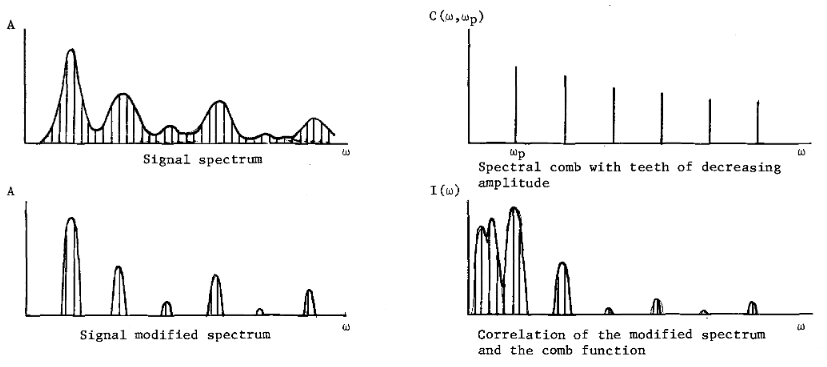
\includegraphics[width=\textwidth]{martin-algo.png}
  \caption{Steps of Martin's algorithm (from \parencite{martin1982comparison}).} \label{fig:martin-algo}
\end{figure}

It reaches maximum when the fundamental frequency of the comb \(\omega_p\) is equal to the fundamental frequency \(\omega_0\) in the power spectrum.

Martin's algorithm is a simple yet effective algorithm.
The \texttt{JSnoori} toolkit implements an enhanced version of Martin's algorithm which additionally takes the energy histogram and voicing jumps into account, etc.

\subsection{SWIPE}

The core idea of Sawtooth Waveform Inspired Pitch Estimator (SWIPE) is that if a signal is periodic with fundamental frequency \(f\), its spectrum must contain peaks at multiples of \(f\)  and valleys in between.

Since each peak is surrounded by two valleys, the average peak-to-valley distance (APVD) for the \(k\)-th peak is defined as

\begin{equation}
  \begin{split}
    d_k(f) & = \frac{1}{2} \left[ \abs{X(kf)} - \abs{X \left( \left(k - \frac{1}{2}\right) f \right)} \right] + \frac{1}{2} \left[ \abs{X(kf)} - \abs{X \left( \left(k + \frac{1}{2} \right) f \right)} \right] \\
      & = \abs{X(kf)} - \frac{1}{2} \left[ \abs{X \left( \left(k - \frac{1}{2}\right) f \right)} + \abs{X \left( \left(k + \frac{1}{2}\right) f \right)} \right]
  \end{split}
\end{equation}

\(X\) is the estimated spectrum of the signal which takes frequency as input and outputs corresponding density.

By averaging over the first \(n\) peaks, we obtain the global APVD, which is to be maximized.

\begin{equation}
  \begin{split}
    D_n(f) & = \frac{1}{n} \sum_{k=1}^{n} d_k(f) \\
      & = \frac{1}{n} \left[ \frac{1}{2} \abs{X \left( \frac{f}{2} \right)} - \frac{1}{2} \abs{X \left( \left(n + \frac{1}{2}\right) f \right)} + \sum_{k=1}^{n} \left( \abs{X(kf)} - \abs{X \left( \left(k - \frac{1}{2}\right) f \right)} \right) \right]
  \end{split}
\end{equation}

There are other improvements such as blurring the harmonics, warping the spectrum and weighting the harmonics.
Please refer to the cited long report \parencite{camacho2007swipe} for all the details.

\subsection{YIN}

YIN is basically a correlation-like method working in the time domain.

A traditional autocorrelation method chooses the highest non-zero-lag peak in the autocorrelation function (ACF, \autoref{eq:acf}) by exhaustive search within a range of lags.

\begin{equation} \label{eq:acf}
  r_t (\tau) = \sum_{j=t+1}^{t+W} x_j x_{j+\tau}
\end{equation}

\(x_t\) is the value of the discrete signal at time index \(t\).
\(r_t (\tau)\) is the autocorrelation function of lag \(\tau\) calculated at time index \(t\), and \(W\) is the integration window size.

It requires elaborated correction algorithms to work well, as the choice of range is vital.
If the actual period lies outside of the chosen range, double or half the correct value is obtained.

YIN instead finds the period by minimizing the difference function \(d_t (\tau)\), which is much less sensitive to amplitude changes while ACF peak amplitudes grow with lag rather than remaining constant when the signal amplitude increases with time.

\begin{equation}
  d_t (\tau) = \sum_{j=1}^W (x_j - x_{j+\tau})^2
\end{equation}

By changing the objective function into the cumulative mean normalized difference function (\autoref{eq:cmndf}), YIN is free from the influence of a strong resonance at the first formant (F1) and eliminates the upper frequency limit of the search range.

\begin{equation} \label{eq:cmndf}
d'_t (\tau) = \begin{cases}
1, \text{if}\ \tau = 0, \\
\dfrac{d_t (\tau)}{\dfrac{1}{\tau} \sum_{j=1}^{\tau} d_t (j)}, \text{otherwise}
\end{cases}
\end{equation}

Absolute threshold, parabolic interpolation and best local estimate further improve YIN's performance.

\newpage

\section{Neural networks}

\subsection{Introduction to neural networks}

Mathematically speaking, (artificial) neural networks are multiple levels of non-linear operations.
By adding more layers and more units within a layer, a deep network can represent functions of increasing complexity.

Most tasks that consist of mapping an input vector to an output vector can be accomplished via relatively deep neural networks, given sufficiently large models and sufficiently large datasets of labeled training samples.

Neural networks (or more recently, \enquote{deep learning}) form a rich and diverse field of research.
A complete description is beyond our scope.
In the following we will introduce the neural network methods involved in our work.

\subsection{Multilayer perceptron}

Multilayer perceptrons, also called feedforward neural networks, are basic but essential models in this field.
They have one or more hidden layers between input and output layer.

\begin{figure}[htbp]
  \centering
  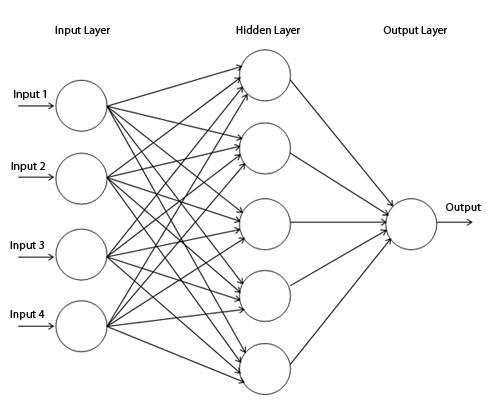
\includegraphics[width=0.5\textwidth]{mlp-example.jpg}
  \caption{An example MLP network with one hidden layer} \label{fig:mlp-example}
\end{figure}

\enquote{Feedforward} means that information flows in one direction from input to output layer (forward).

Every node calculates the weighted sum of its inputs \(\mathbf{x}\) and apply some activation function \(f\) to get the output \(y\), \( y = f (\mathbf{w}^\intercal \mathbf{x} + b) \).

Rectified linear unit (ReLU), defined as \(f(x) = \max(0, x)\), is the optimal choice for activation function inside MLP nowadays.

\begin{figure}[htbp]
  \centering
  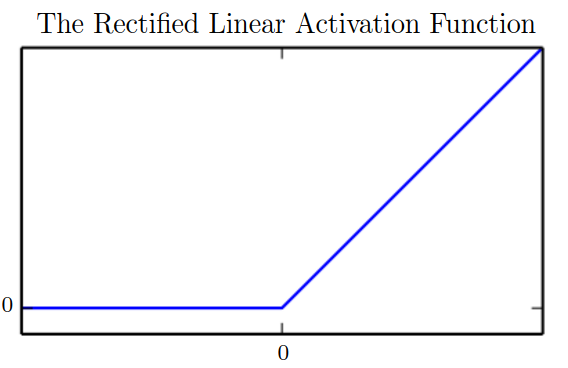
\includegraphics[width=0.5\textwidth]{relu.png}
  \caption{Rectified linear unit (ReLU).} \label{fig:relu}
\end{figure}

It has several advantages over \(\mathrm{tanh}\), etc.

\begin{itemize}
  \item piecewise polynomial non-linearity
  \item no vanishing gradient problem or exploding effect
  \item sparse activation
\end{itemize}

\subsection{Recurrent networks and long short-term memory}

There are no feedback connections in multilayer perceptrons by which outputs of the model are fed back into itself.
In order to remember information over time, recurrent connections must be adopted.

Recurrent neural network (RNN) is a popular choice for processing sequential data.
Its chain-like structure is able to capture temporal dependencies.

\begin{figure}[htbp]
  \centering
  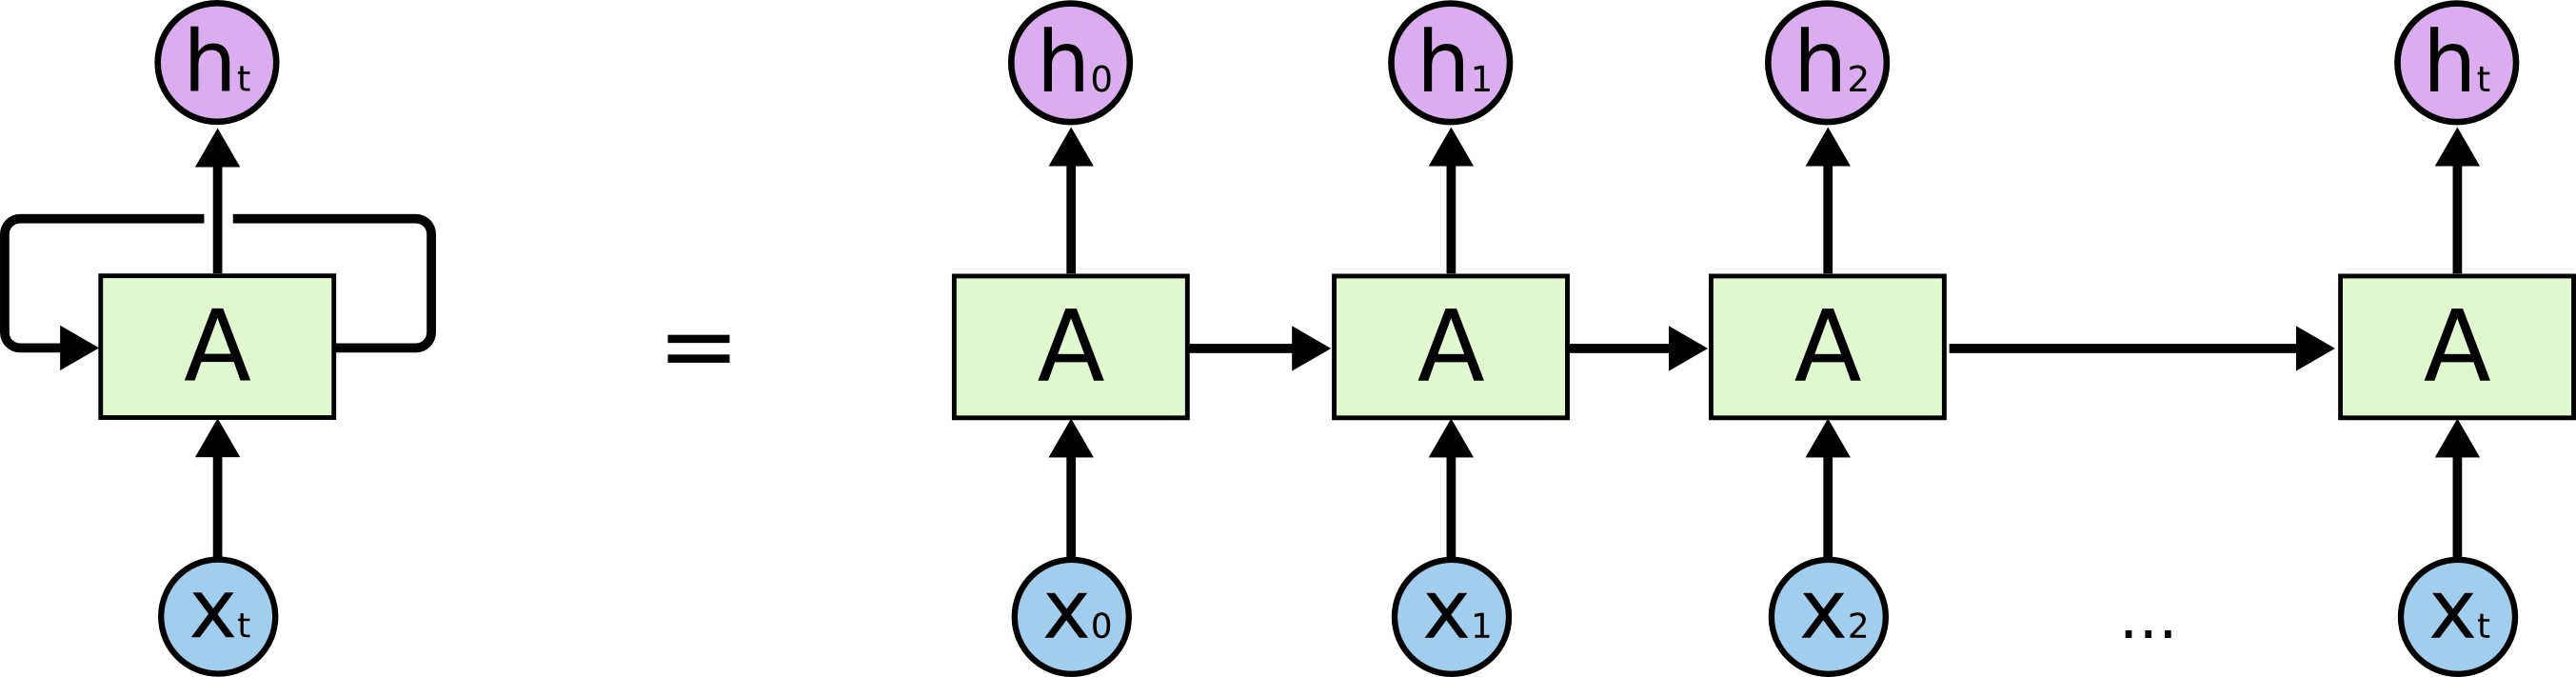
\includegraphics[width=\textwidth]{RNN-unrolled.png}
  \caption{An unrolled recurrent neural network.} \label{fig:rnn-intro}
\end{figure}

The structures of recurrent neural networks are rather flexible, depending on the task and especially on which operations should be conducted on sequences.

\begin{figure}[htbp]
  \centering
  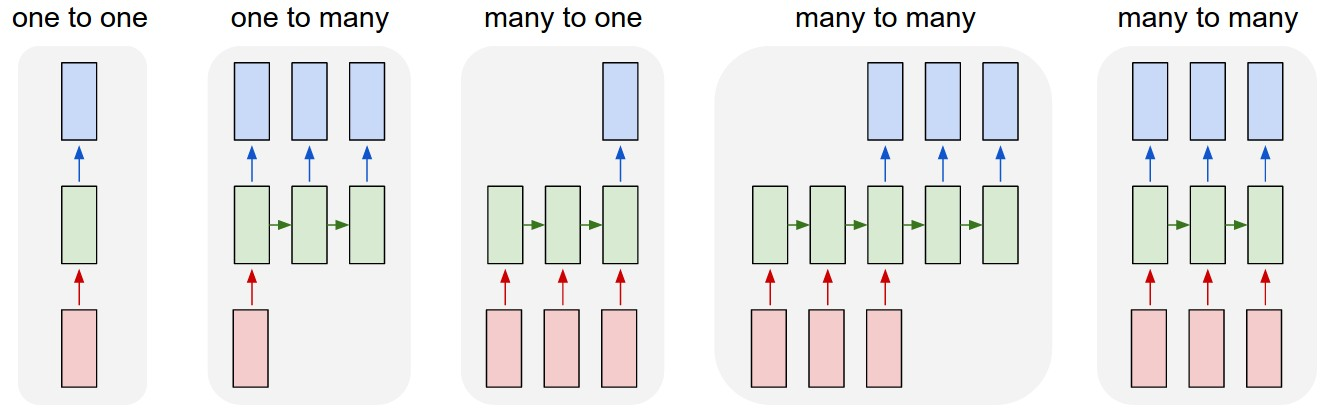
\includegraphics[width=\textwidth]{rnns.jpeg}
  \caption[Various recurrent structures compared with MLP.]{Various recurrent structures compared with MLP (leftmost).
    Each rectangle is a vector and arrows represent functions (e.g.\, matrix multiply).
    Input vectors are in red, output vectors are in blue and green vectors hold the RNN's state \protect\footnotemark.}
  \label{fig:rnns}
\end{figure}

\footnotetext{\url{http://karpathy.github.io/2015/05/21/rnn-effectiveness/}}

\begin{itemize}
  \item one to many: tasks such as generating captions from images.
  \item many to one: sequence classification, including sentiment analysis and \textbf{our task}.
  \item many to many: neural machine translation, neural network TTS, etc.
\end{itemize}

Bengio \parencite{bengio1994learning} shows that, though theoretically possible, in practice it's very hard to tune vanilla RNNs to handle long-term dependencies.

Long short-term memory network (LSTM) is a variant of RNN explicitly designed to tackle the long-term dependency problem.

\begin{figure}[htbp]
  \centering
  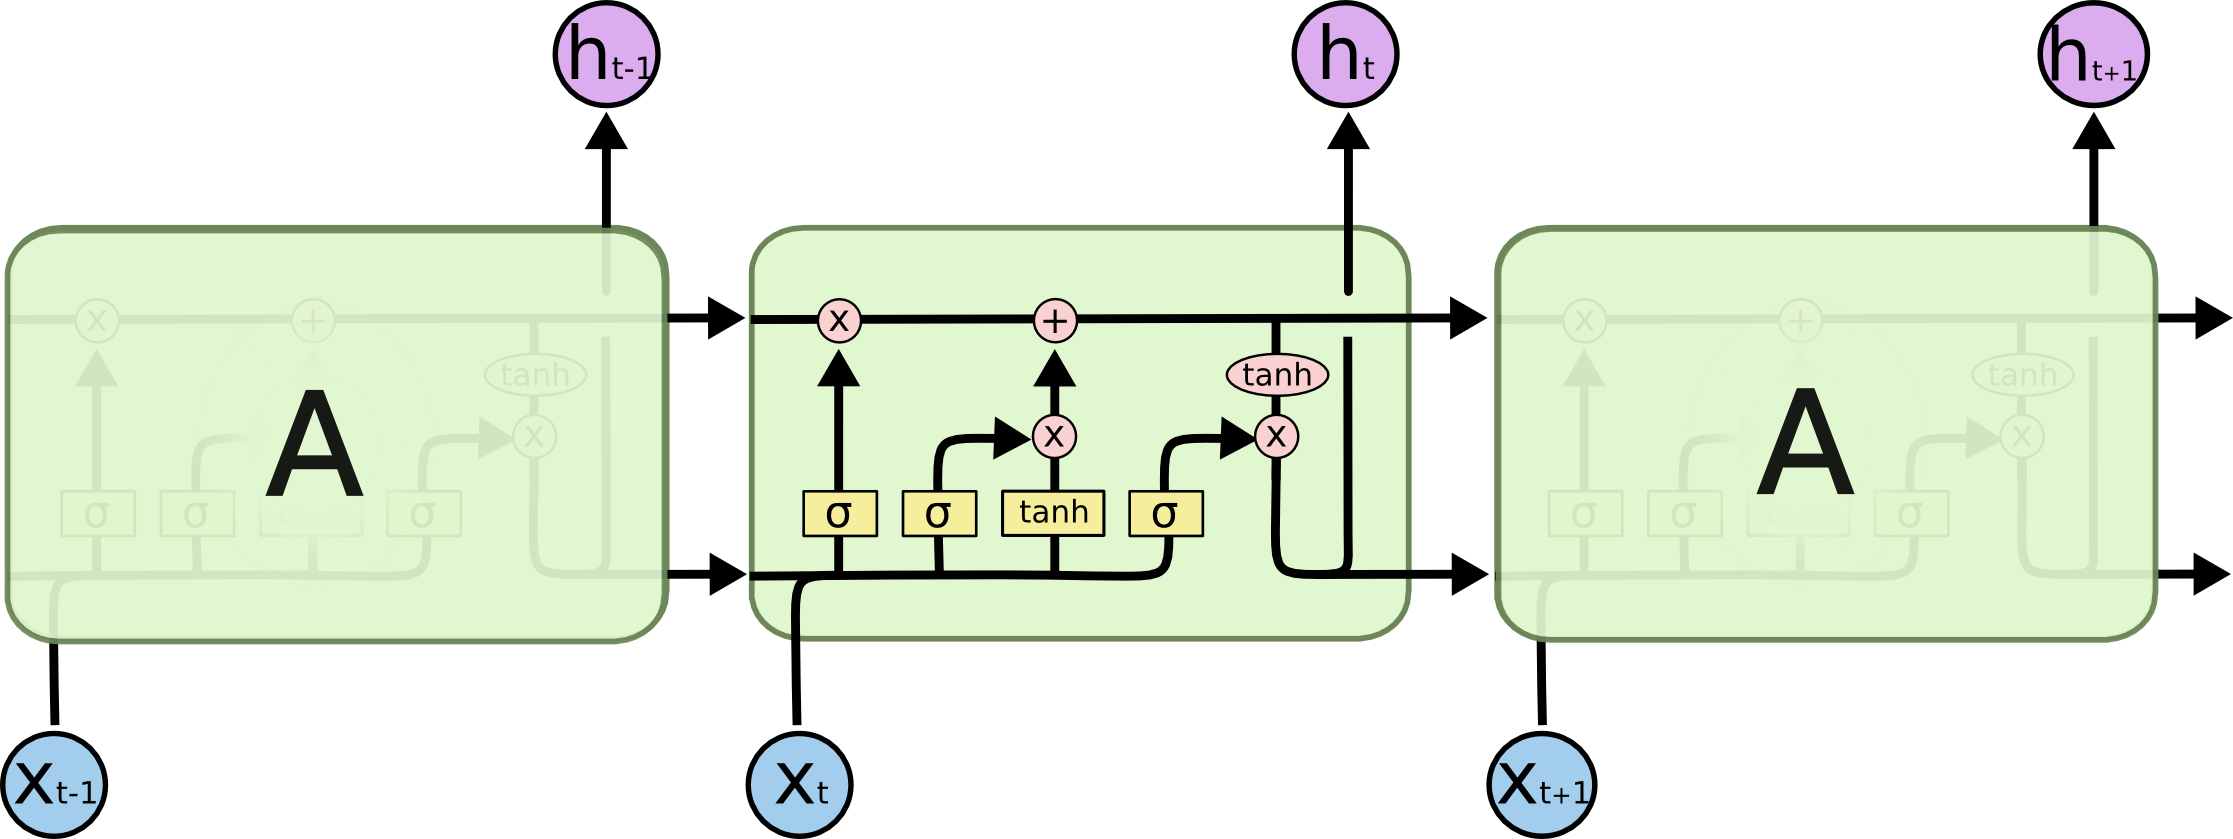
\includegraphics[width=\textwidth]{LSTM3-chain.png}
  \caption[Details of an LSTM cell.]{Details of an LSTM cell\protect\footnotemark.} \label{fig:lstm-intro}
\end{figure}

\footnotetext{\url{http://colah.github.io/posts/2015-08-Understanding-LSTMs/}}

The cell state (horizontal line running through the top of the diagram) enables information to flow into the next time step freely.
Any modification to the cell state is regulated by \enquote{gates}, composed of a \texttt{sigmoid} (\(\sigma\)) layer and a point-wise operation.
From left to right are \enquote{forget gate}, \enquote{input gate} and \enquote{output gate}, respectively.

Forget gate decides the proportion \(f_t\) of previous cell state to keep, individually on each dimension.

\begin{equation*}
  f_t = \sigma (W_f \cdot [h_{t-1}, x_t] + b_f)
\end{equation*}

Input gate produces new candidate values \(\tilde{C_t}\) and an input proportion \(i_t\).

\begin{align*}
  i_t & = \sigma (W_i \cdot [h_{t-1}, x_t] + b_i) \\
  \tilde{C_t} & = \mathrm{tanh} (W_C \cdot [h_{t-1}, x_t] + b_C)
\end{align*}

Then cell state is updated to \(C_t\) and new hidden output \(h_t\) is produced, regulated by output gate.

\begin{align*}
  C_t & = f_t * C_{t-1} + i_t * \tilde{C_t} \\
  o_t & = \sigma (W_o \cdot [h_{t-1}, x_t] + b_o) \\
  h_t & = o_t * \mathrm{tanh}(C_t)
\end{align*}

\enquote{\(\cdot\)} is the dot product of two vectors and \enquote{\(*\)} is multiplying by scalar element-wise.

\subsection{Training of neural networks}

Neural networks are usually trained using gradient-based optimization methods, to minimize the cost function (also called loss function).
A cost function measures the quality of a particular set of parameters based on how well the induced scores agree with ground truth labels.

Parameters are updated by backpropagation, which is a way of computing gradients of expressions through recursive application of chain rule.

\newpage

\section{Confidence measures}

While accuracy or average error rate have been used as standard metrics to characterize the performance of various systems, it is always useful to have a sense of correctness of each result.

\bigskip

Mathematically speaking, it is

\begin{center}
  \textit{the probability of the result to be correct}
\end{center}

or

\begin{center}
  \textit{the true posterior probability} \(P (c_i = 1 | X)\)
\end{center}

in Bayesian approach.
\(c_i = 1\) means the class label is \(c_i\) for sample \(X\).

\subsection{Confidence measures in speech recognition}

In speech processing, besides the task of fundamental frequency estimation, another notable use case for confidence measures is the field of automatic speech recognition (ASR).

Any applicable real-world ASR system must be able to distinguish error prone results from its candidate outputs.
This requires the ASR systems to automatically assess reliability for every decision made by the systems.
Researchers propose to calculate a score between 0 and 1, i.e.\, confidence measure, to quantify this reliability.

A confidence measure can be calculated on every recognized word, indicating how likely it is to match the audio segment, or on the whole result corresponding to the input utterance.
It is vital for achieving \emph{robust speech recognition} and is still a trending topic.

\subsection{Approaches to confidence measures}

There are roughly three major categories of methods for computing confidence measures in ASR \parencite{jiang2005confidence}.

\subsubsection{Combination of predictor features}

Any feature can be called a predictor if its probabilistic distribution of correctly recognized words is clearly distinct from that of misrecognized words.
The predictor features may have to be collected within the recognition process.

Some common predictor features include \textit{N-best related scores}, \textit{acoustic stability}, \textit{phoneme or word durations}, \textit{language model score} and \textit{parsing results}.

Then all predictor features are combined in a certain way to generate a single score to indicate correctness of the recognition decision.
This can be done by various popular machine learning algorithms, but usually the combination methods cannot significantly improve over the best predictor feature.

\subsubsection{Hypothesis testing}

The confidence measure is formulated as a statistical hypothesis testing problem, under the framework of utterance verification.

For a given speech segment \(X\) , assume that an ASR system recognizes it as word \(W\) which is represented by a model \(\lambda_W\).
Then two complementary hypotheses are proposed, namely null hypothesis \(H_0\) and the alternative hypothesis \(H_1\).

\begin{itemize}
  \item \(H_0\): \(X\) is correctly recognized and truly comes from model \(\lambda_w\).
  \item \(H_1\): \(X\) is wrongly classified and is not from model \(\lambda_w\).
\end{itemize}

Then test \(H_0\) against \(H_1\) to determine whether to accept the recognition result or reject it.
The final solution ends up with calculating and evaluating likelihood ratio or Bayes factors.

\subsubsection{As posterior probability}

Conventional ASR systems find the most likely sequence of words \(\hat{W}\) for acoustic observation \(X\) by \textit{maximum a posterior} decision rule.

\begin{equation}
  \begin{split}
    \hat{W} & = \argmax_{W \in \Sigma} p(W|X) \\
      & = \argmax_{W \in \Sigma} \frac{p(X|W) p(W)}{p(X)} \\
      & = \argmax_{W \in \Sigma} p(X|W) p(W)
  \end{split}
\end{equation}
\(\Sigma\) is the set of all permissible sentences.

In theory, the posterior probability \(p(W|X)\) is a good confidence measure.

However, most practical ASR systems ignore \(p(X)\) during decision making so raw ASR scores are inadequate.
And actually it is impossible to margin over all combinations of words, phonemes, noises, and other events to get \(p(X)\).

Therefore, approximate methods are adopted.
Usually, one word lattice or graph is generated by the ASR decoder for every utterance.
Then the posterior probability of each recognized word or the entire hypothesized sentence can be calculated based on the word-graph from an additional post-processing stage.

\subsection{Confidence measures and neural networks}

As shown above, it is a complicated task to calculate the posterior probabilities \enquote{online} during speech recognition.

However, posterior probabilities may also be estimated \enquote{offline}, under the framework of classification, when we have ground truth telling us whether the results are correct.

\bigskip

\begin{mdframed}
\begin{theorem}
  Bayesian probabilities are estimated when desired network outputs are 1 of M (one output unity, all others zero) and a squared-error or cross-entropy cost function is used. \parencite{richard1991neural}
\end{theorem}
\end{mdframed}

\begin{itemize}
  \item Neural network binary classifiers having only one node with \texttt{sigmoid} activation function in the output layer, are able to output a value between 0 and 1 for classification decision.
    The higher the value, the more it favors the positive class.
  \item For multiclass classification problems, usually \texttt{softmax} activation function is used in the output layer.
    The class with the highest activation value (also between 0 and 1) gets output.
\end{itemize}

According to the theorem proved in \parencite{richard1991neural}, \textbf{the above activation values estimate Bayesian a posteriori probabilities, acting directly as confidence measures}, as long as we choose squared-error or cross-entropy as cost function.

\bigskip

Under such a framework, multiclass neural network classifiers are applicable for estimating posterior probabilities for different candidate words.

And in our work about fundamental frequency estimation, it's a binary classification problem between \enquote{estimation is correct} and \enquote{estimation is incorrect}.
What we want is the posterior probability for \enquote{estimation is correct}.

\chapter{Corpora}

\section{Speech corpus}

The Pitch Tracking Database from Graz University of Technology (PTDB-TUG) \parencite{pirker2011pitch} is used throughout the remainder of this thesis.

This dataset contains microphone and laryngograph signals of 20 English native speakers reading out sentences from the TIMIT corpus \parencite{garofolo1993darpa}.
Both microphone signals and laryngograph signals were recorded at \SI{48}{\kilo\hertz} sampling rate, \SI{16}{\bit} resolution, with the type of encoding signed PCM.

Additionally, reference pitch trajectories extracted on the laryngograph signals using the RAPT algorithm \parencite{talkin1995robust} are provided.
In total it has \num{4720} recorded utterances.

It is the first audio corpus that meets the following requirements:

\begin{itemize}
  \item a substantial amount of speech data composed of phonetically rich sentences that allows for meaningful training of speaker-dependent models
  \item a variety of female and male speakers such that a multi-pitch tracker can be evaluated seriously
\end{itemize}

\textbf{The latter feature is crucial to our work since frequency ranges of female and male voices differ a lot.} The gender distribution is 50:50, and age varies from 22 to 48 years as described in the specifications.

\bigskip

In the corpus, audio files are encoded in \texttt{WAV} format and the filename contains signal type, speaker ID and sentence ID\@.
Only microphone signals are used for testing.
For any microphone signal file \texttt{mic\_*.wav}, the corresponding file containing reference values is \texttt{ref\_*.f0}, in CSV-like format.

According to the default pitch extraction script and the Snack Sound Toolkit\footnote{\url{http://www.speech.kth.se/snack/}} manual, indices of the reference values start at \SI{16}{\milli\second} and have a uniform interval of \SI{10}{\milli\second} until the end.

\section{Noise corpus}

The PTDB-TUG corpus contains only clean signals recorded inside a recording studio.
Additional noise audios are needed in latter steps of our work.
We pick five noise audio files from the NOISEX-92 corpus \parencite{varga1993assessment}, which is often used in the field of automatic speech recognition.

\begin{itemize}
  \item \texttt{babble.wav}: 100 people speaking in a canteen and individual voices are slightly audible.
  \item \texttt{factory1.wav}: recorded near plate-cutting and electrical welding equipment in a factory.
  \item \texttt{factory2.wav}: recorded in a car production hall.
  \item \texttt{pink.wav}: acquired by sampling high-quality analog noise generator (Wandel \& Goltermann).
    Exhibits equal energy per \SI{1/3}{octave}.
  \item \texttt{white.wav}: acquired by sampling high-quality analog noise generator (Wandel \& Goltermann).
    Exhibits equal energy per \si{\hertz} bandwidth.
\end{itemize}

They have the same duration of \SI{235}{\second}, resolution of \SI{16}{\bit} and sampling rate at \SI{19.98}{\kilo\hertz}.

\section{A unified sampling rate}

\texttt{JSnoori} requires that input audio files are sampled at \SI{16}{\kilo\hertz}.
We use \texttt{SoX}\footnote{\url{http://sox.sourceforge.net/}} to conduct the conversion.

\chapter{Empirical Analyses of the Algorithms} \label{emp-aly}

We conduct a series of empirical analyses of performance of the fundamental frequency estimation algorithms.
This is done by altering the audio files in various ways, running the algorithms and comparing the results with reference values to calculate error rates.

Estimation results and reference values are technically time series at (usually) uniform intervals along the time axis of signals.
They don't necessarily have the same starting point or interval.
So we interpolate estimation results to obtain matching values at reference indices.
In order to maintain the clear boundaries between voiced and unvoiced frames and avoid introducing erroneous interpolated intermediate values, and since the intervals are very short even in voiced areas, \textbf{nearest-neighbor interpolation} is applied throughout.

\begin{figure}[htbp]
  \centering
  \begin{subfigure}{\textwidth}
    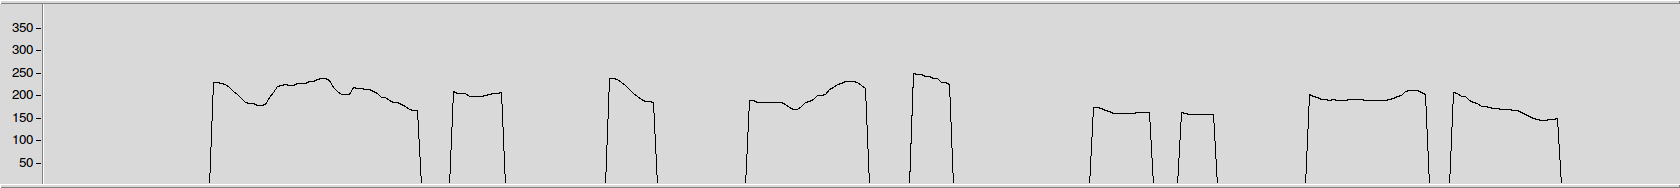
\includegraphics[width=\textwidth]{f0s-lp.png}
    \caption{Linear interpolation}
    \label{fig:f0s-lp}
  \end{subfigure}

  \begin{subfigure}{\textwidth}
    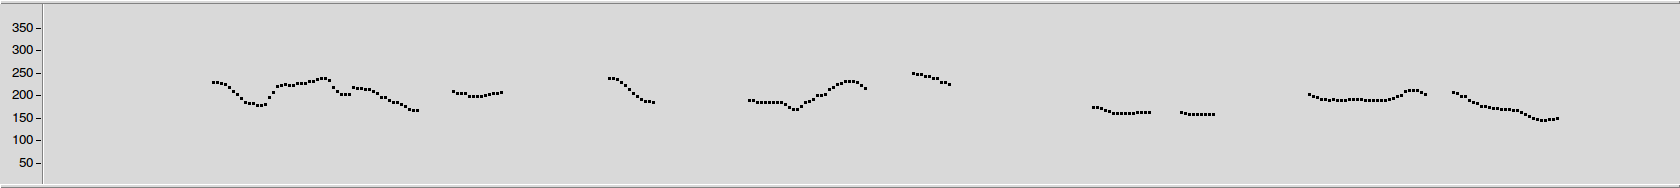
\includegraphics[width=\textwidth]{f0s-real.png}
    \caption{Actual values}
    \label{fig:f0s-real}
  \end{subfigure}

  \caption[Data plotting options in Wavesurfer.]{Wavesurfer is able to plot time series with connecting lines, analogous to linear interpolation.
    \textbf{The actual fundamental frequency values within steep areas are either zero or the neighboring nonzero value, not on the connecting lines.}}
  \label{fig:f0s}
\end{figure}

We set the maximum deviation percentage from reference values to be \SI{20}{\percent}, within this range the estimation results are considered correct.

The different experiments we conduct are as follows.
Elaborated figures and statistics are provided.

\newpage

\section{Apply offsets to indices}

Fundamental frequency estimation algorithms usually compute features over a sliding window and use the centers of the windows as time indices for estimated values.
This is sometimes inaccurate, as the proper indices may deviate from the centers, and the specific offsets depend on the internal mechanisms and implementations of the algorithms, which are not always explicitly documented.

We use grid search to empirically find the optimal offset for every algorithm implemented in \texttt{JSnoori}: before interpolating the estimation results, pick an offset from some range and apply it to all the indices.
The optimal offset will minimize the error rate.

\begin{figure}[htbp]
  \centering
  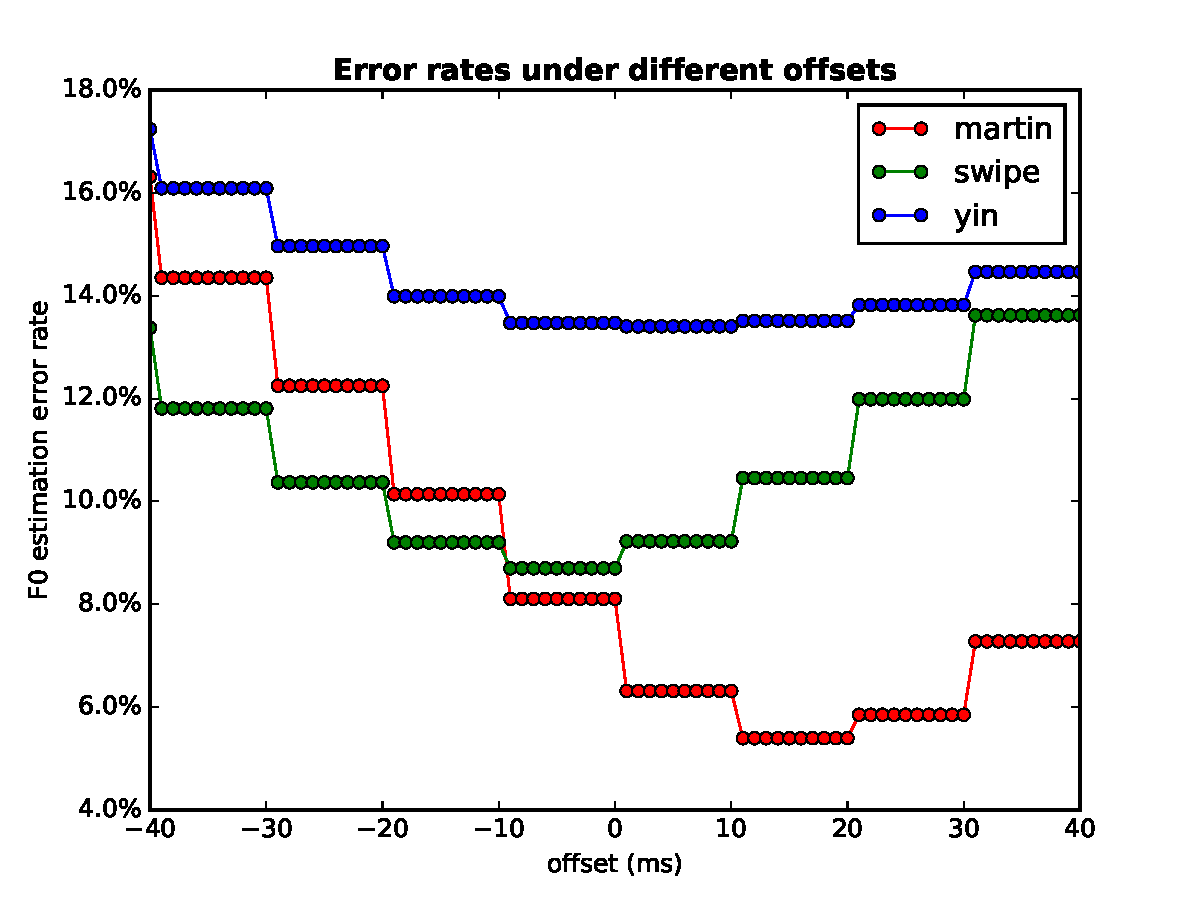
\includegraphics[width=0.9\textwidth]{error_rates_vs_offsets.pdf}
  \caption{Error rates under different offsets.} \label{fig:offsets}
\end{figure}

\autoref{fig:offsets} shows the error rates when different offsets are applied.
There are plateaus in the curves which means that nearest-neighbor interpolation works.
The optimal offsets we find are shown in \autoref{tab:offsets}.

\begin{table}[htbp]
  \centering
  \begin{tabular}{cSSS}
  	\toprule
  	             Algorithm              & {Martin's} & {SWIPE} & {YIN} \\
  	\midrule
  	Optimal offset (\si{\milli\second}) & 16         & -4      & 6     \\
  	\bottomrule
  \end{tabular}
  \caption{Optimal offsets for the three algorithms.} \label{tab:offsets}
\end{table}

We will apply these optimal offsets throughout the following experiments.

\newpage

\section{Modify signal levels}

Error rates are expected to rise when signal levels are lowered.

\begin{figure}[htbp]
  \centering
  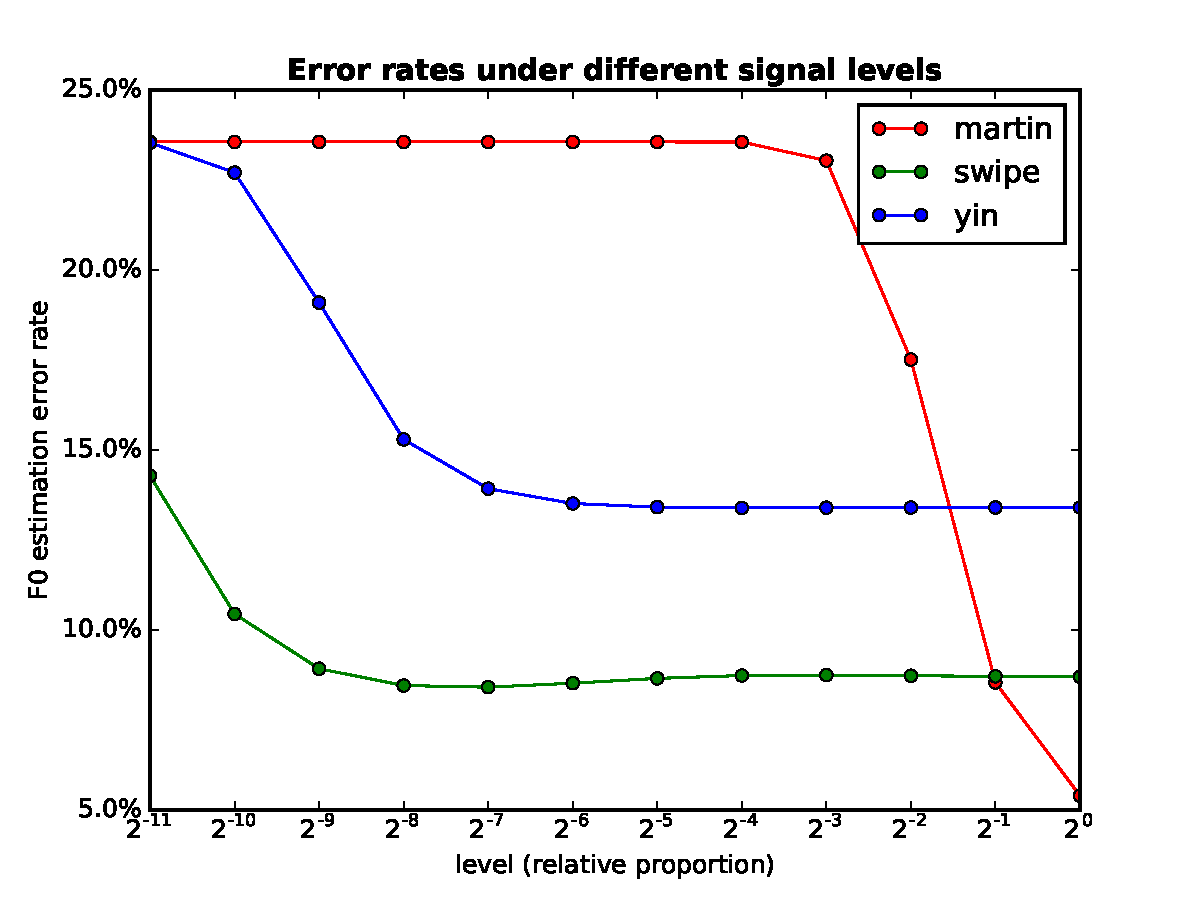
\includegraphics[width=0.9\textwidth]{error_rates_vs_signal_levels.pdf}
  \caption{Error rates under different signal levels.} \label{fig:levels}
\end{figure}

We use the \texttt{SoX} utility to adjust the signals to different levels (scale the signal values).
The resulting error rates are plotted in \autoref{fig:levels}.

\begin{mdframed}
\textbf{Comment and Analysis}

\bigskip

For all three algorithms, error rates converge to about \SI{23.56}{\percent} when signal level approaches zero.
This is the proportion of voiced samples (i.e.\, values \( > \SI{0}{\hertz} \)) in reference values.
\textbf{When signal level is very low, the algorithms output \SI{0}{\hertz} for all data points, thus only the estimation results aligned to voiced reference values are wrong.}

\bigskip

From the plot we can see that Martin's algorithm performs well when signal level is unmodified, but is very sensitive to further changes.
In contrast, SWIPE and YIN's performance are rather steady and the results are always usable since real-life signal level changes are much smaller.
(Also, SWIPE works better than YIN in this task.) \textbf{This is because that enhanced Martin's algorithm explicitly takes energy of the signal into account while SWIPE and YIN do not.
Starting from \(2^{-3}\), enhanced Martin's algorithm decides that most of the frames are unvoiced, which is overpessimistic.}
\end{mdframed}

\newpage

\section{Add noise by level}

We then evaluate the effects of noise.
\texttt{SoX} is used again to add noise types to the original signals.

This is done by scaling the signal level of a noise file and then mixing it with the original audio file.
To avoid clipping, we calculate the sum of peak amplitudes (maximum absolute value) of the two files before mixing.
If it exceeds the largest value that can be represented (though clipping may not actually happen because the two maxima usually don't occur at the same time index), we apply another scaling on the two files.

\begin{equation}
  Y = \alpha S + \alpha \lambda N, \quad
  \alpha = \begin{cases}
    \mathrlap{1}\hphantom{\frac{1}{\mathrm{pa}(S) + \mathrm{pa}(\lambda N)}}, \mathrm{pa}(S) + \mathrm{pa}(\lambda N) < 1 \\
    \frac{1}{\mathrm{pa}(S) + \mathrm{pa}(\lambda N)}, \mathrm{pa}(S) + \mathrm{pa}(\lambda N) \geq 1
  \end{cases}
\end{equation}

\(Y\), \(S\) and \(N\) are output, speech, and noise signals, respectively.
\(\alpha\) and \(\lambda\) are scale factors.
\(\mathrm{pa}()\) is the function returning peak amplitude.

We first choose \(\lambda\) from \{0, 0.0125, 0.025, 0.05, 0.1, 0.2, 0.4, 0.8\} and apply the white noise generated by SoX, which always has the maximum possible peak amplitude 1.
Results are shown in \autoref{fig:white-noise}.

\begin{figure}[htbp]
  \centering
  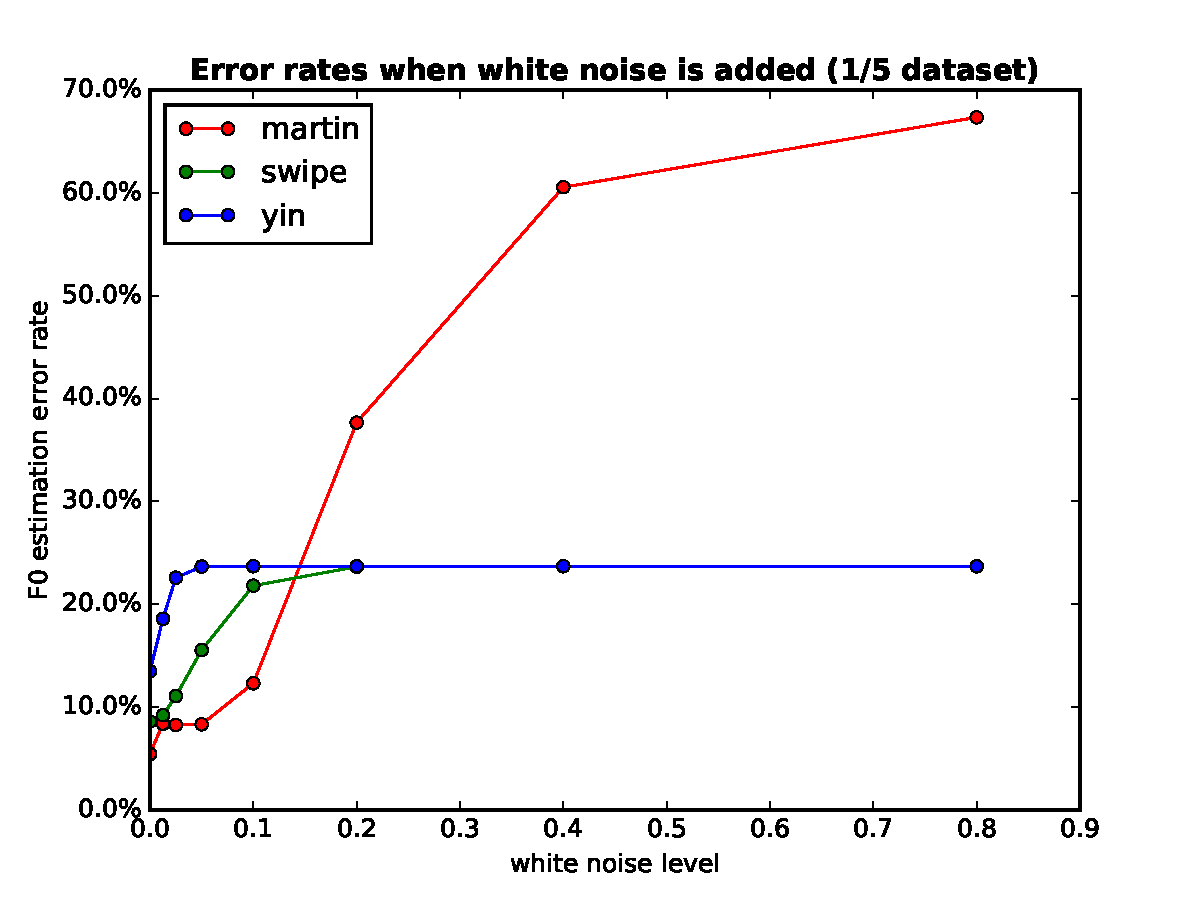
\includegraphics[width=0.9\textwidth]{error_rates_white_noise_added.pdf}
  \caption[Error rates when white noise is added.]{Error rates when white noise is added.
    White noise level corresponds to \(\lambda\).}
  \label{fig:white-noise}
\end{figure}

Then we randomly sample noises from the five noise audio files in the NOISEX-92 corpus: \texttt{babble.wav}, \texttt{factory1.wav}, \texttt{factory2.wav}, \texttt{pink.wav} and \texttt{white.wav}.
The last one is also white noise but with a different volume.

Results are shown in \autoref{fig:random-noise-same-algorithm} and \autoref{fig:random-noise-same-audio}\footnote{Legends indicate \texttt{(noise, algorithm)} combinations.
The same applies to all figures of this type.} These statistics objectively reflect the three algorithms' robustness to different kinds of noise at real-life signal levels.

Noise levels all correspond to \(\lambda\), the five noise signals have very different signal levels or volumes.

\begin{mdframed}
\textbf{Comment and Analysis} (\autoref{fig:white-noise})

\bigskip

Martin's algorithm is more resistant to distortion when the noise level is relatively low, and has better performance than SWIPE and YIN\@.
Though its error rate continues rising afterwards, SWIPE and YIN's error rates converge to the proportion of voiced samples again so the results are meaningless, too.
\textbf{This kind of \enquote{blowup} is again caused by enhanced Martin's algorithm's decision mechanism based on energy.
More and more noise saturates the signal and enhanced Martin's algorithm does a lot of useless estimations on originally unvoiced frames.}

\bigskip

YIN's performance drops very quickly.
\textbf{It is basically correlation-like and therefore less robust to noise as the waveform changes drastically.}
\end{mdframed}

\begin{mdframed}
\textbf{Comment and Analysis} (\autoref{fig:random-noise-same-algorithm} and \autoref{fig:random-noise-same-audio})

\bigskip

\autoref{fig:random-noise-same-algorithm} further verifies our first conclusion about \autoref{fig:white-noise}.
The higher the volume of a noise signal, the more quickly the error rate of enhanced Martin's algorithm rises.
\texttt{white.wav} has much lower volume than the white noise generated by \texttt{SoX}, so the error rate even doesn't change much all the way.

\bigskip

In general, all three fundamental frequency estimation algorithms are more easily influenced by real-life noise than generated noise signals (\texttt{pink.wav} and \texttt{white.wav}) when the noises are of realistic volumes or \enquote{recorded as it is}.

\end{mdframed}

\begin{figure}[htbp]
  \centering
  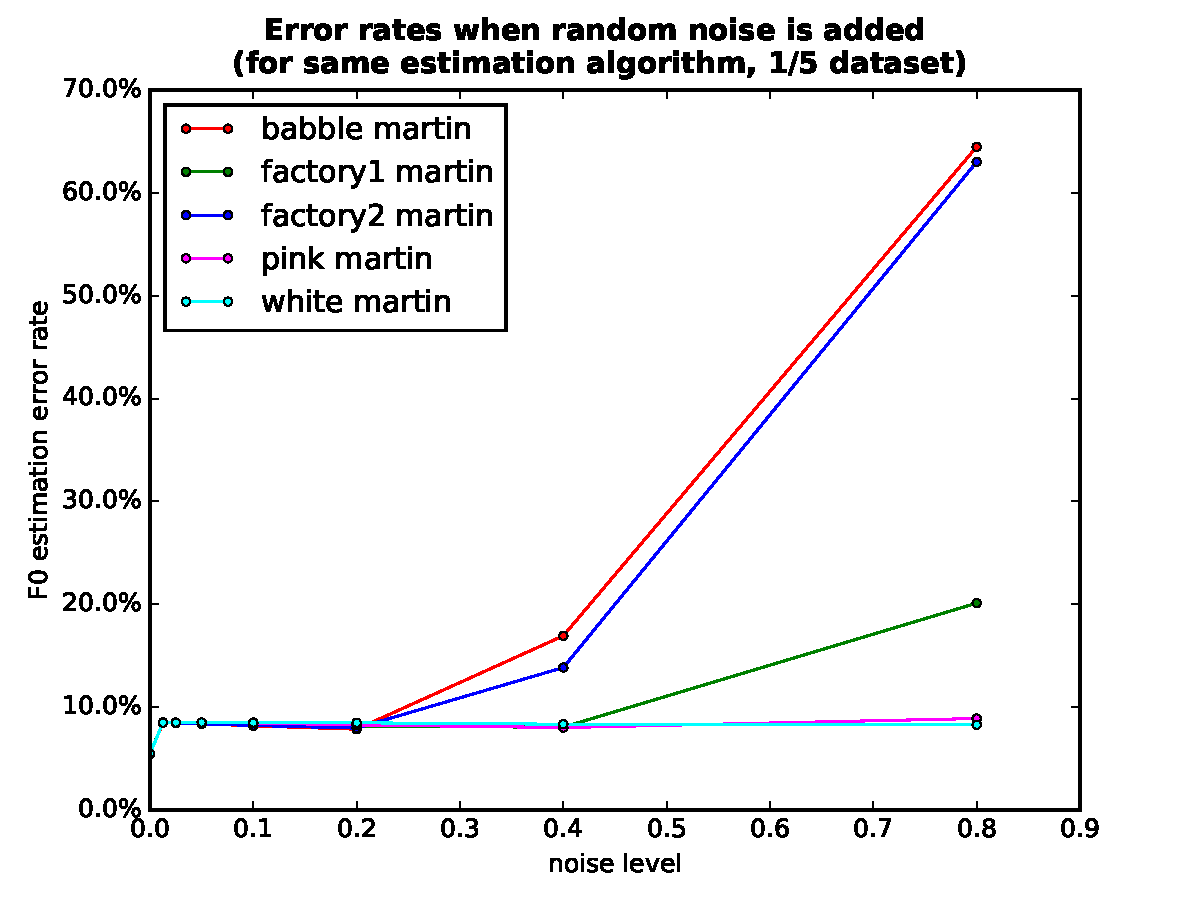
\includegraphics[width=0.65\textwidth]{error_rates_random_noise_martin.pdf}
  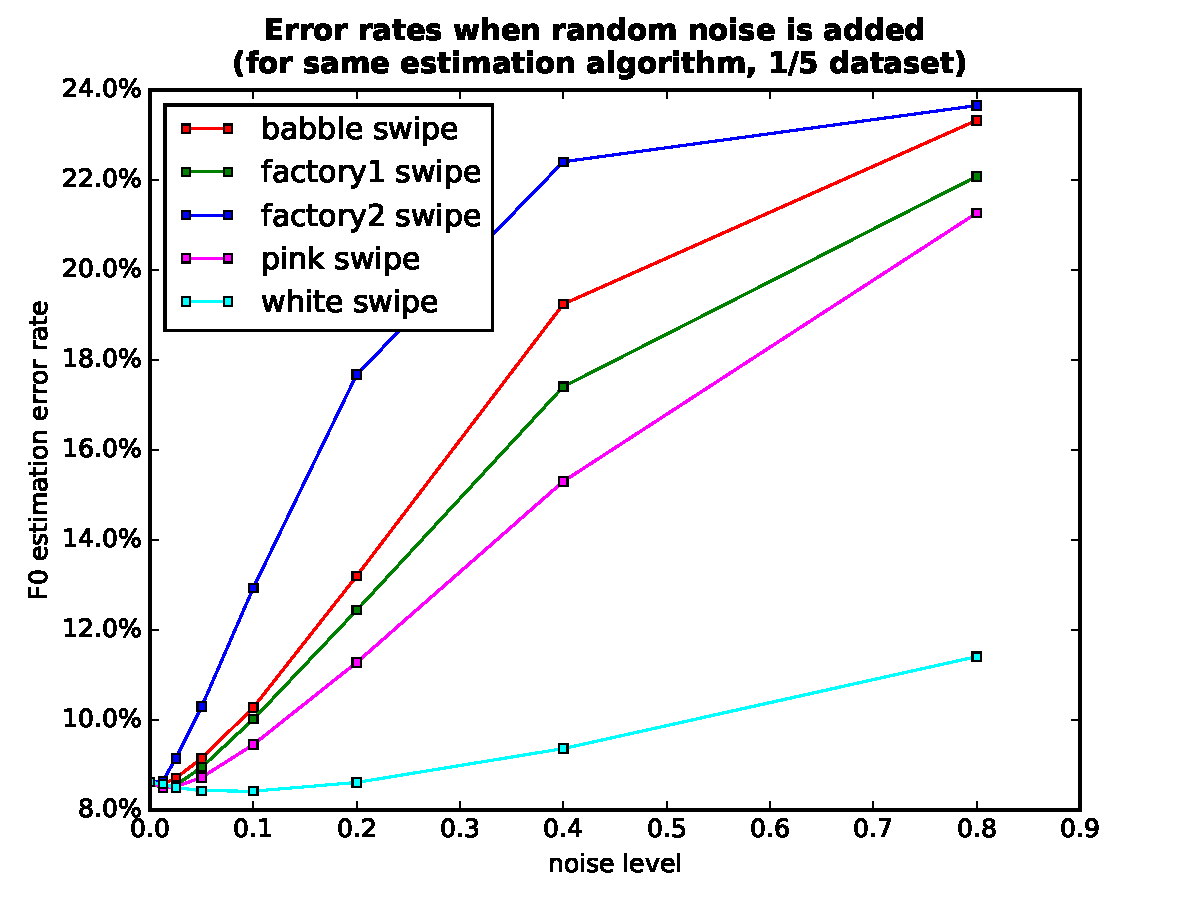
\includegraphics[width=0.65\textwidth]{error_rates_random_noise_swipe.pdf}
  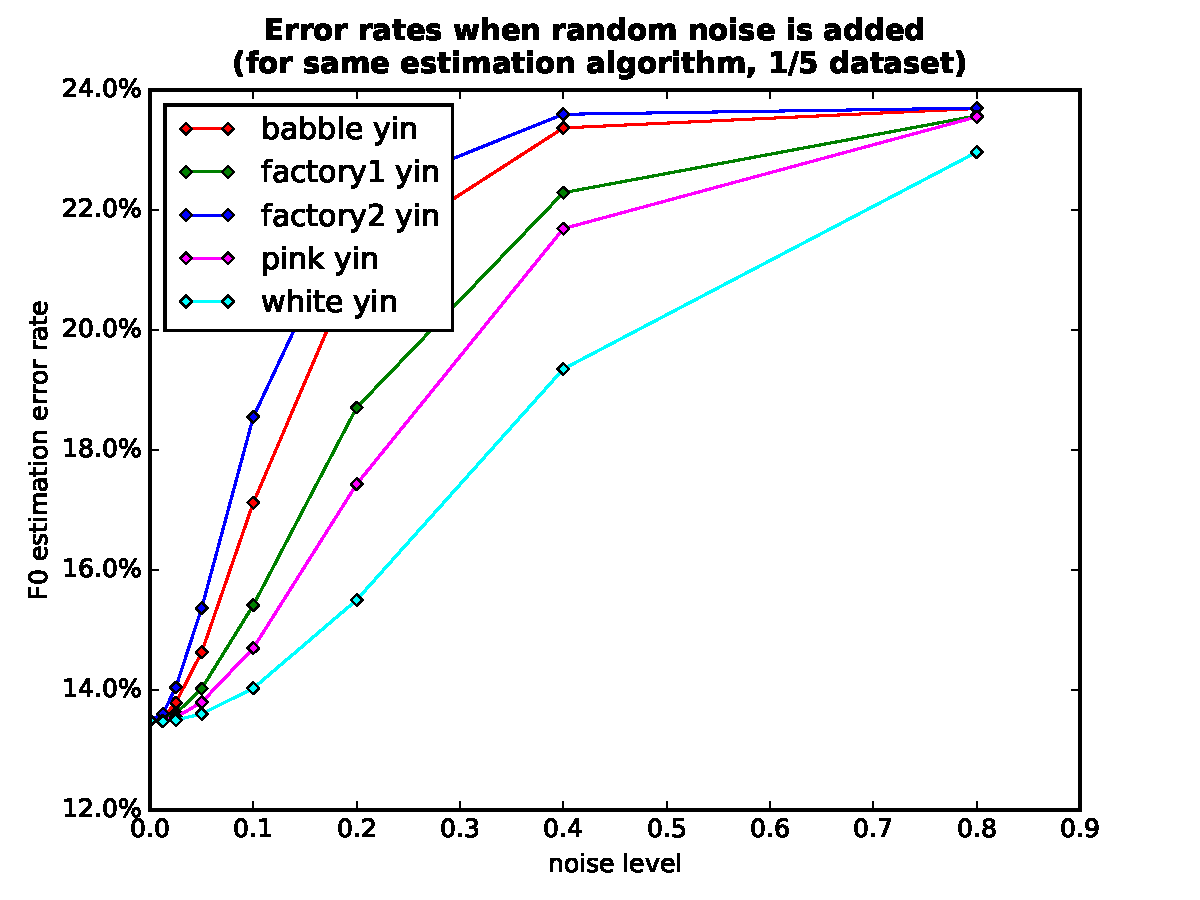
\includegraphics[width=0.65\textwidth]{error_rates_random_noise_yin.pdf}
  \caption[Error rates of the same algorithm when random noise is sampled from different audios.]{Error rates of the same algorithm when random noise is sampled from different audio signals.
    Subfigures have different y-axis limits.}
  \label{fig:random-noise-same-algorithm}
\end{figure}

\begin{figure}[htbp]
  \centering
  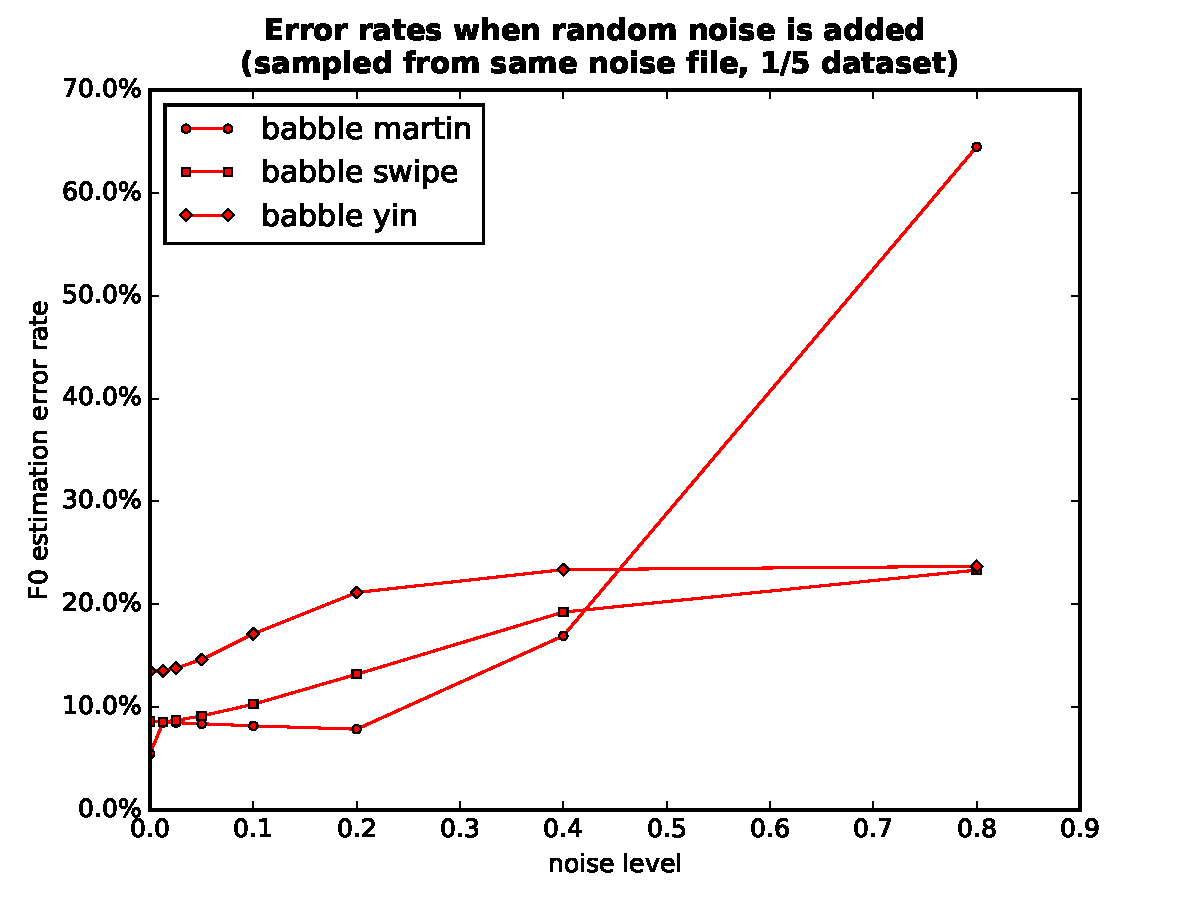
\includegraphics[width=0.49\textwidth]{error_rates_random_noise_babble.pdf}
  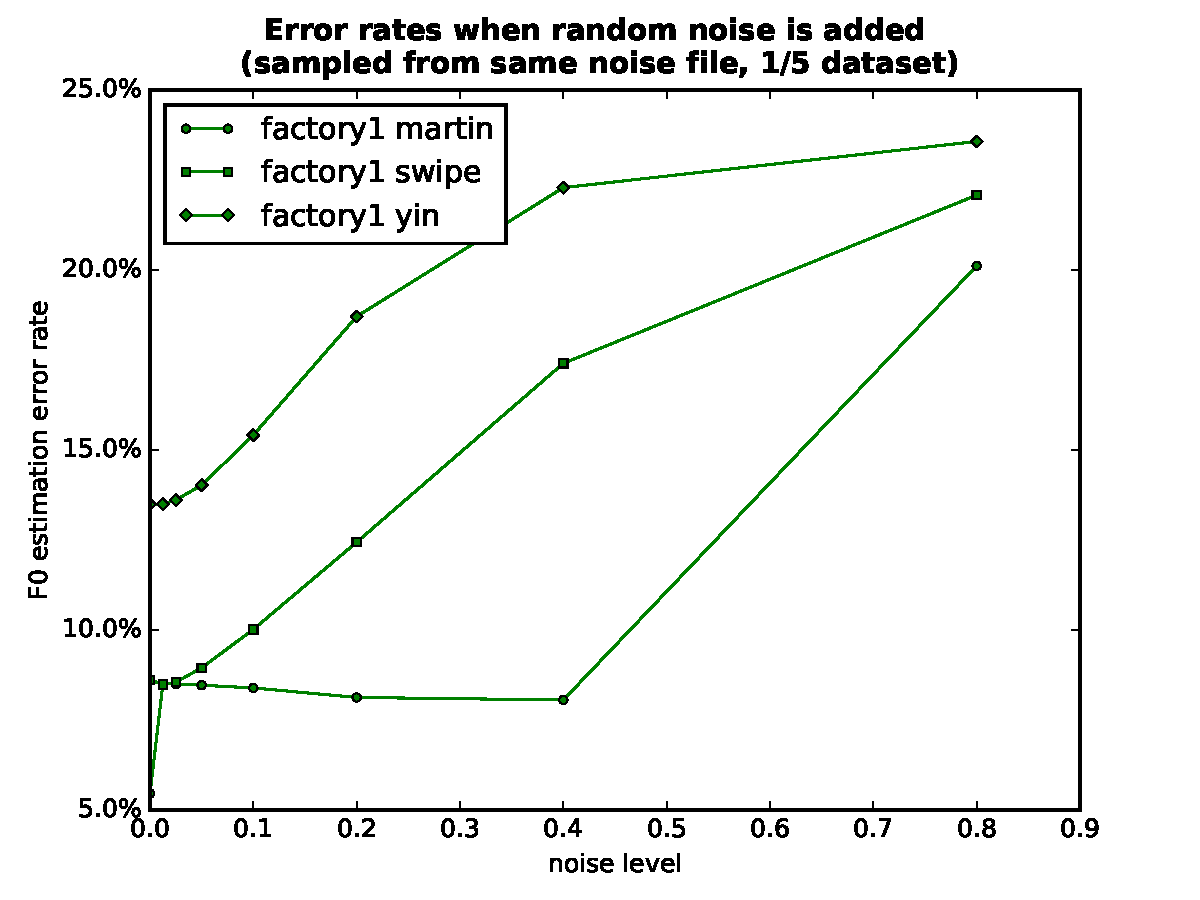
\includegraphics[width=0.49\textwidth]{error_rates_random_noise_factory1.pdf}
  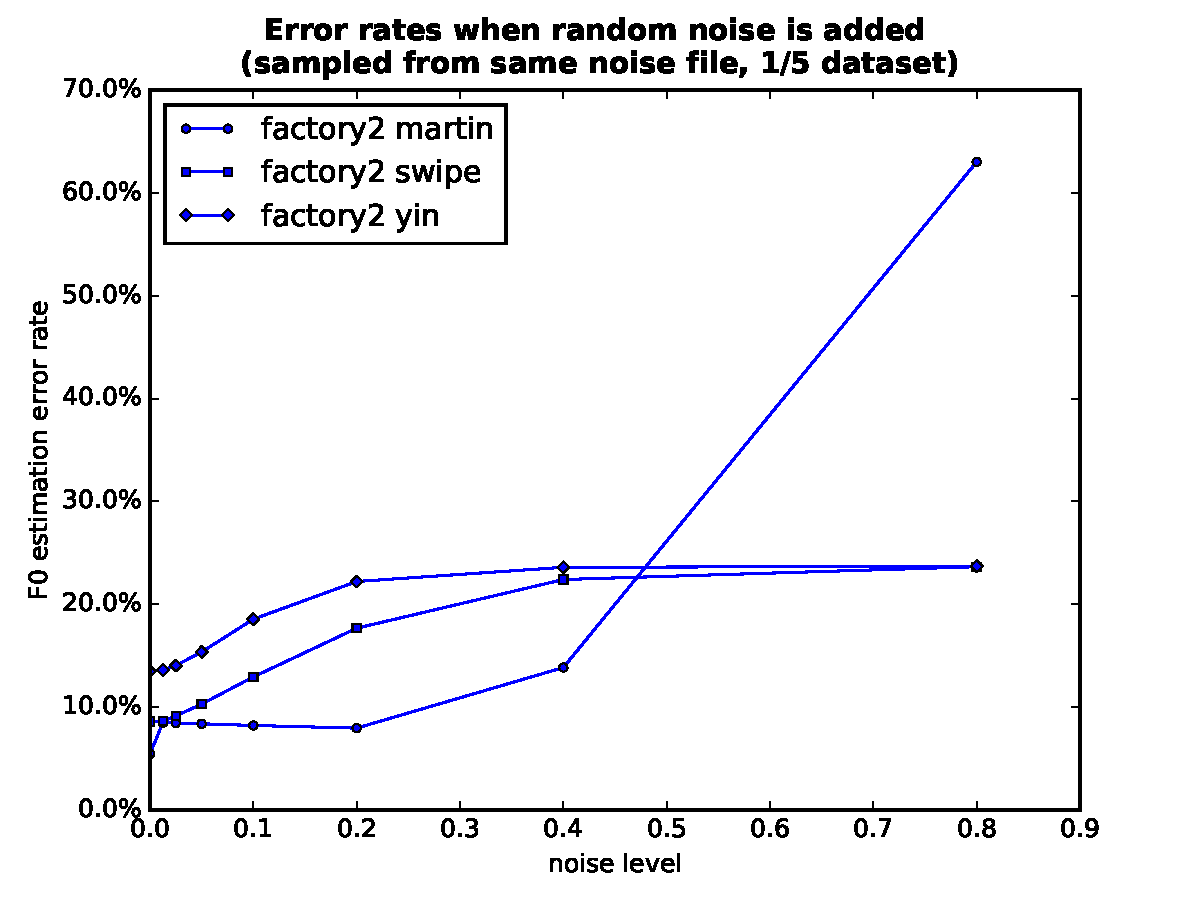
\includegraphics[width=0.49\textwidth]{error_rates_random_noise_factory2.pdf}
  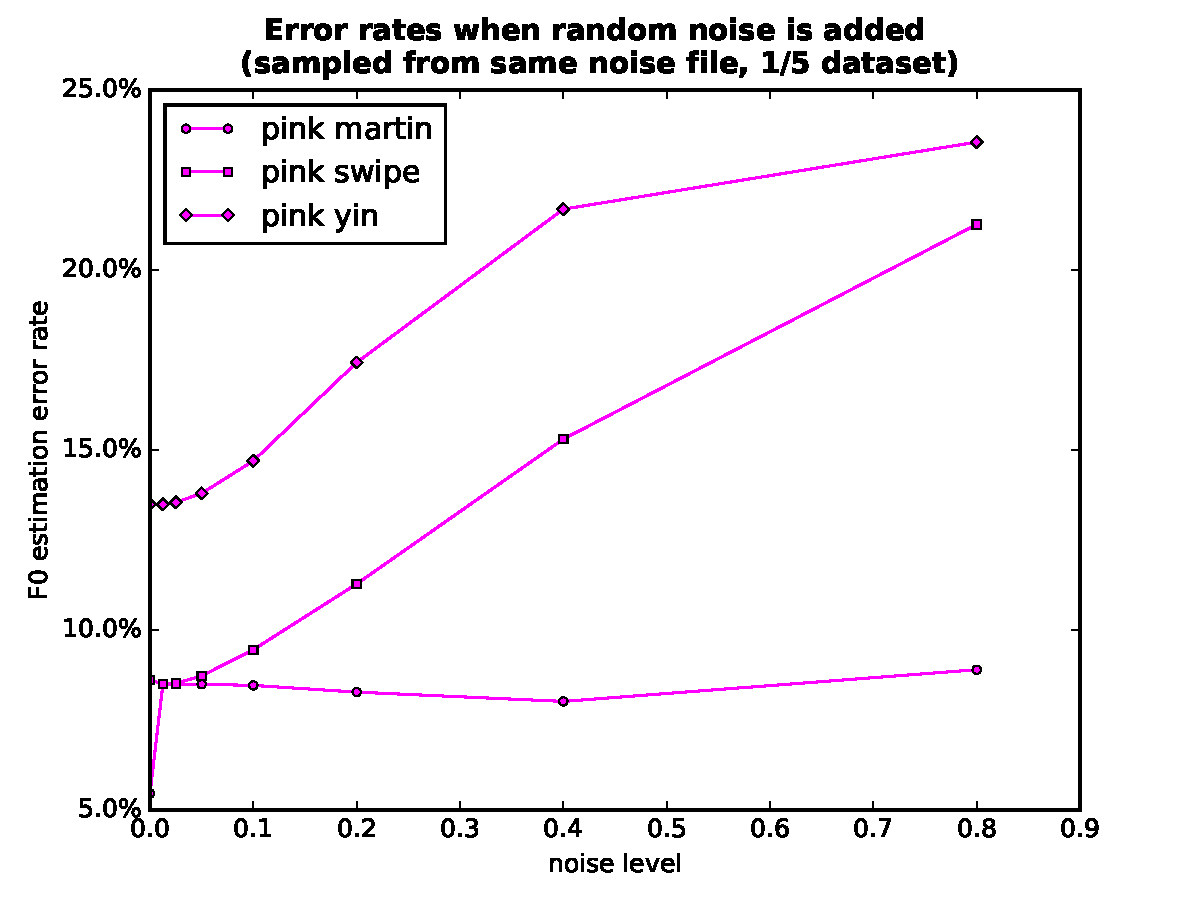
\includegraphics[width=0.49\textwidth]{error_rates_random_noise_pink.pdf}
  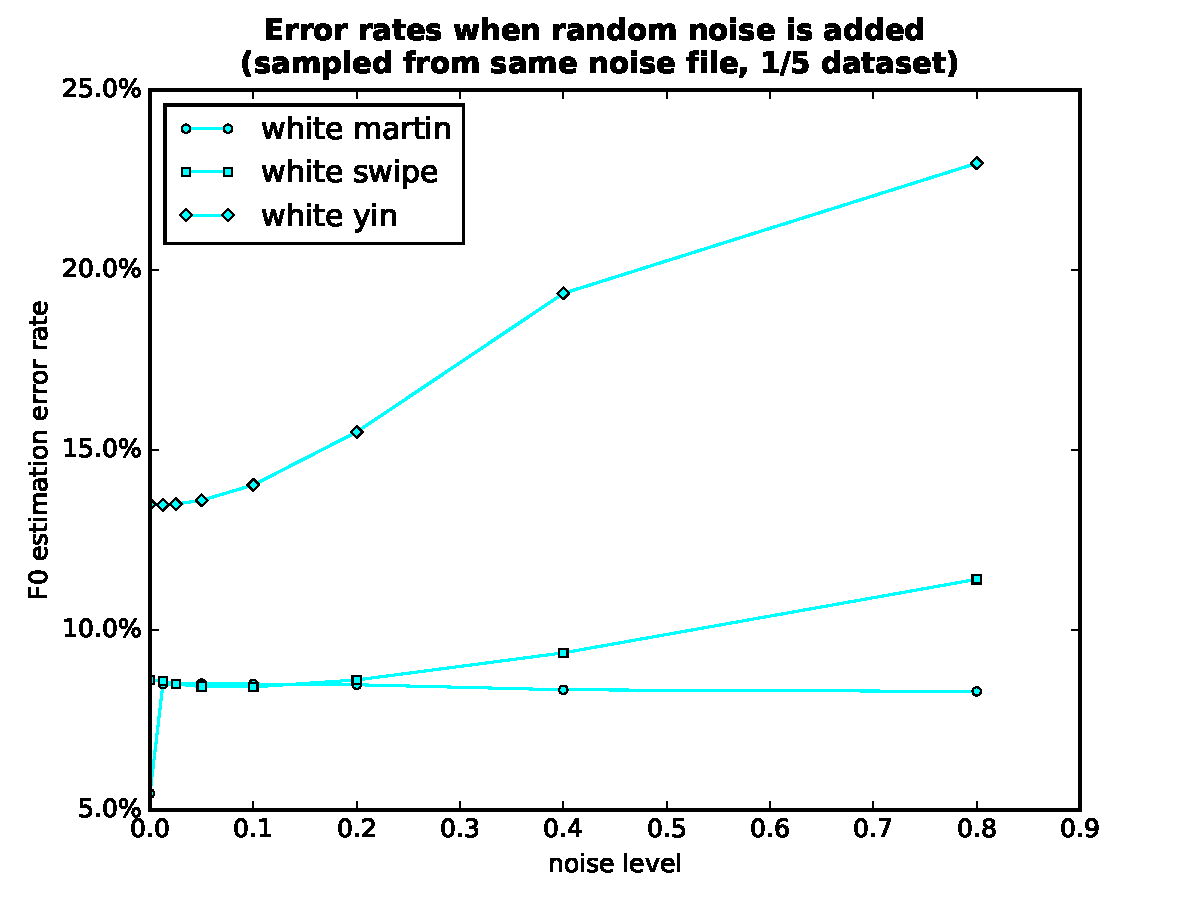
\includegraphics[width=0.49\textwidth]{error_rates_random_noise_white.pdf}
  \caption[Error rates of different algorithms when random noise is sampled from the same audio.]{Error rates of different algorithms when random noise is sampled from the same audio.
    Subfigures have different y-axis limits.}
  \label{fig:random-noise-same-audio}
\end{figure}

\newpage

\section{Add noise by signal-to-noise ratio}

A tool named \texttt{FaNT - Filtering and Noise Adding Tool}\footnote{\url{http://dnt.kr.hs-niederrhein.de/index964b.html}} enables us to add a noise signal at a given signal-to-noise ratio (SNR), which makes the results (in \autoref{fig:snr}) easier to interpret and more numerically referable.
Noise signals are first sampled across the five noise files.
All audio files need to be converted to RAW format first, which is also done by \texttt{SoX}.

\begin{figure}[htbp]
  \centering
  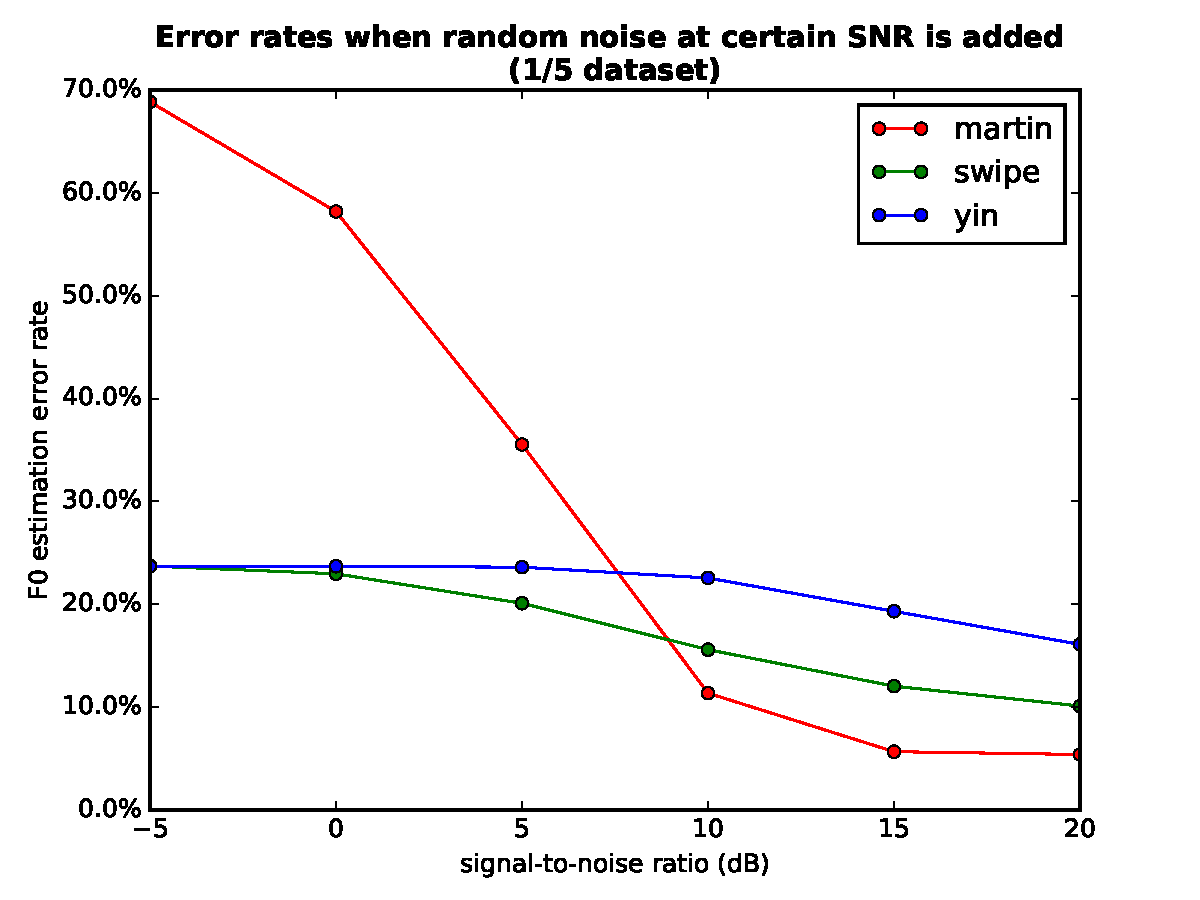
\includegraphics[width=0.9\textwidth]{error_rates_vs_snrs.pdf}
  \caption{Error rates when random noise at certain SNR is added.} \label{fig:snr}
\end{figure}

\begin{figure}[htbp]
  \centering
  \begin{subfigure}{0.7\textwidth}
    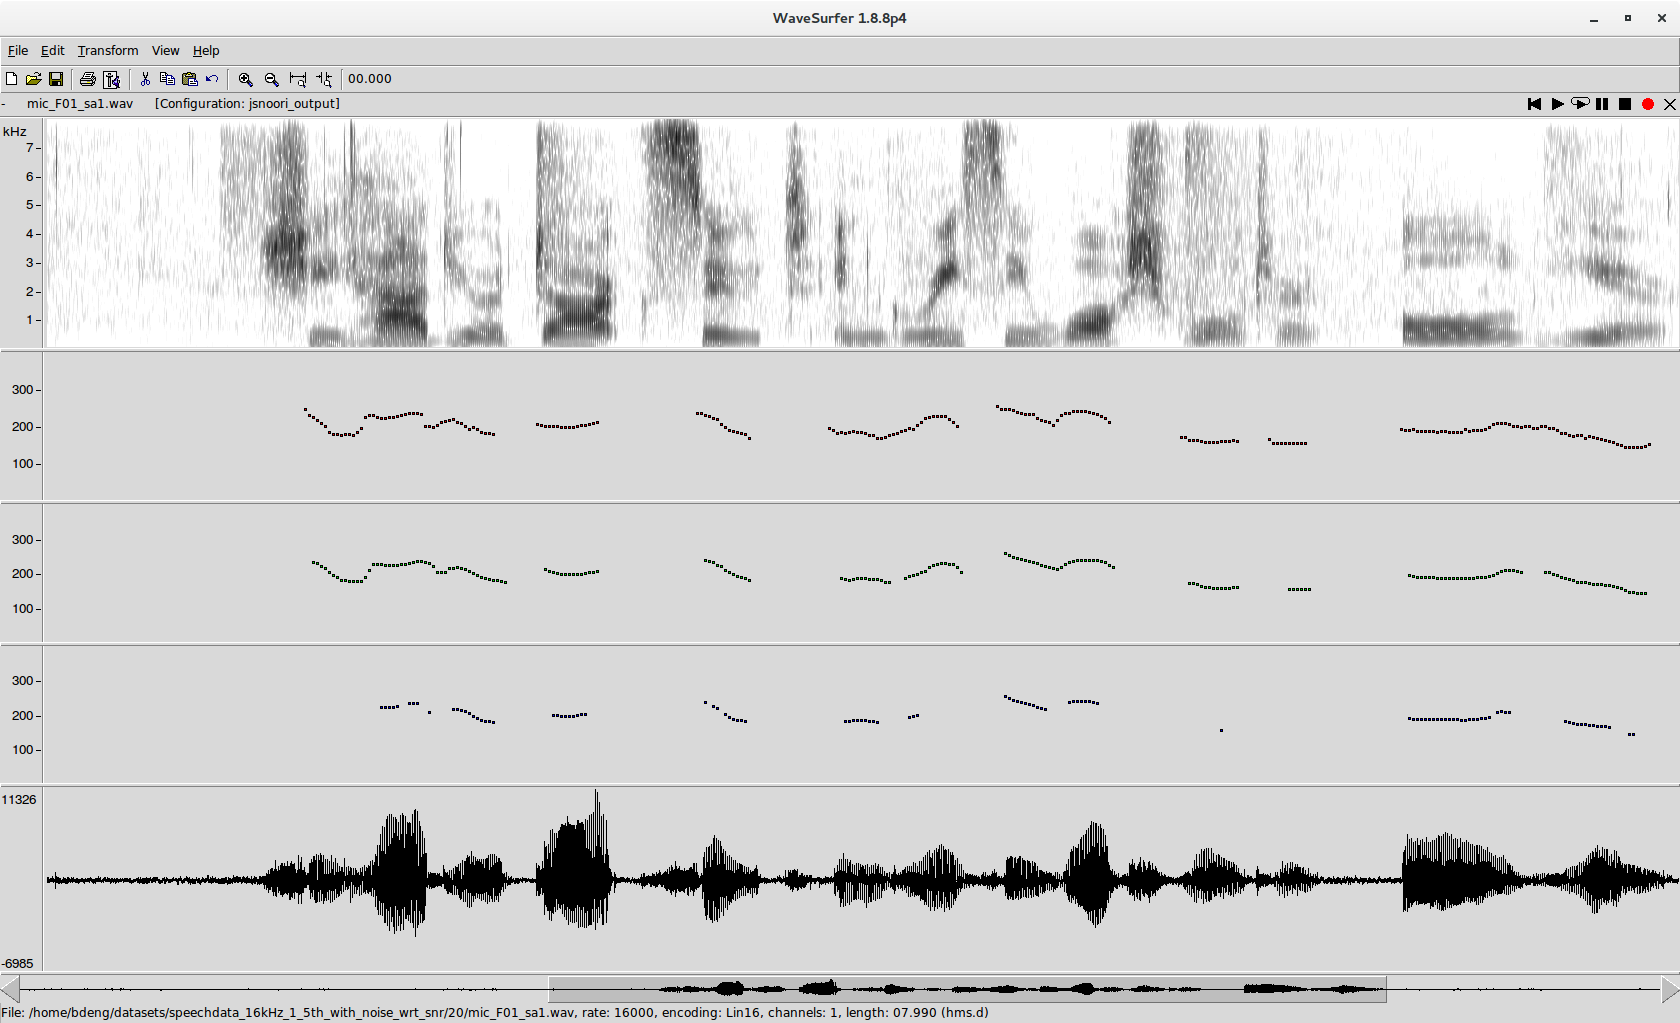
\includegraphics[width=\textwidth]{snr_20dB.png}
    \caption{SNR = \SI{20}{dB}}
    \label{fig:snr-compare-20db}
  \end{subfigure}

  \begin{subfigure}{0.7\textwidth}
    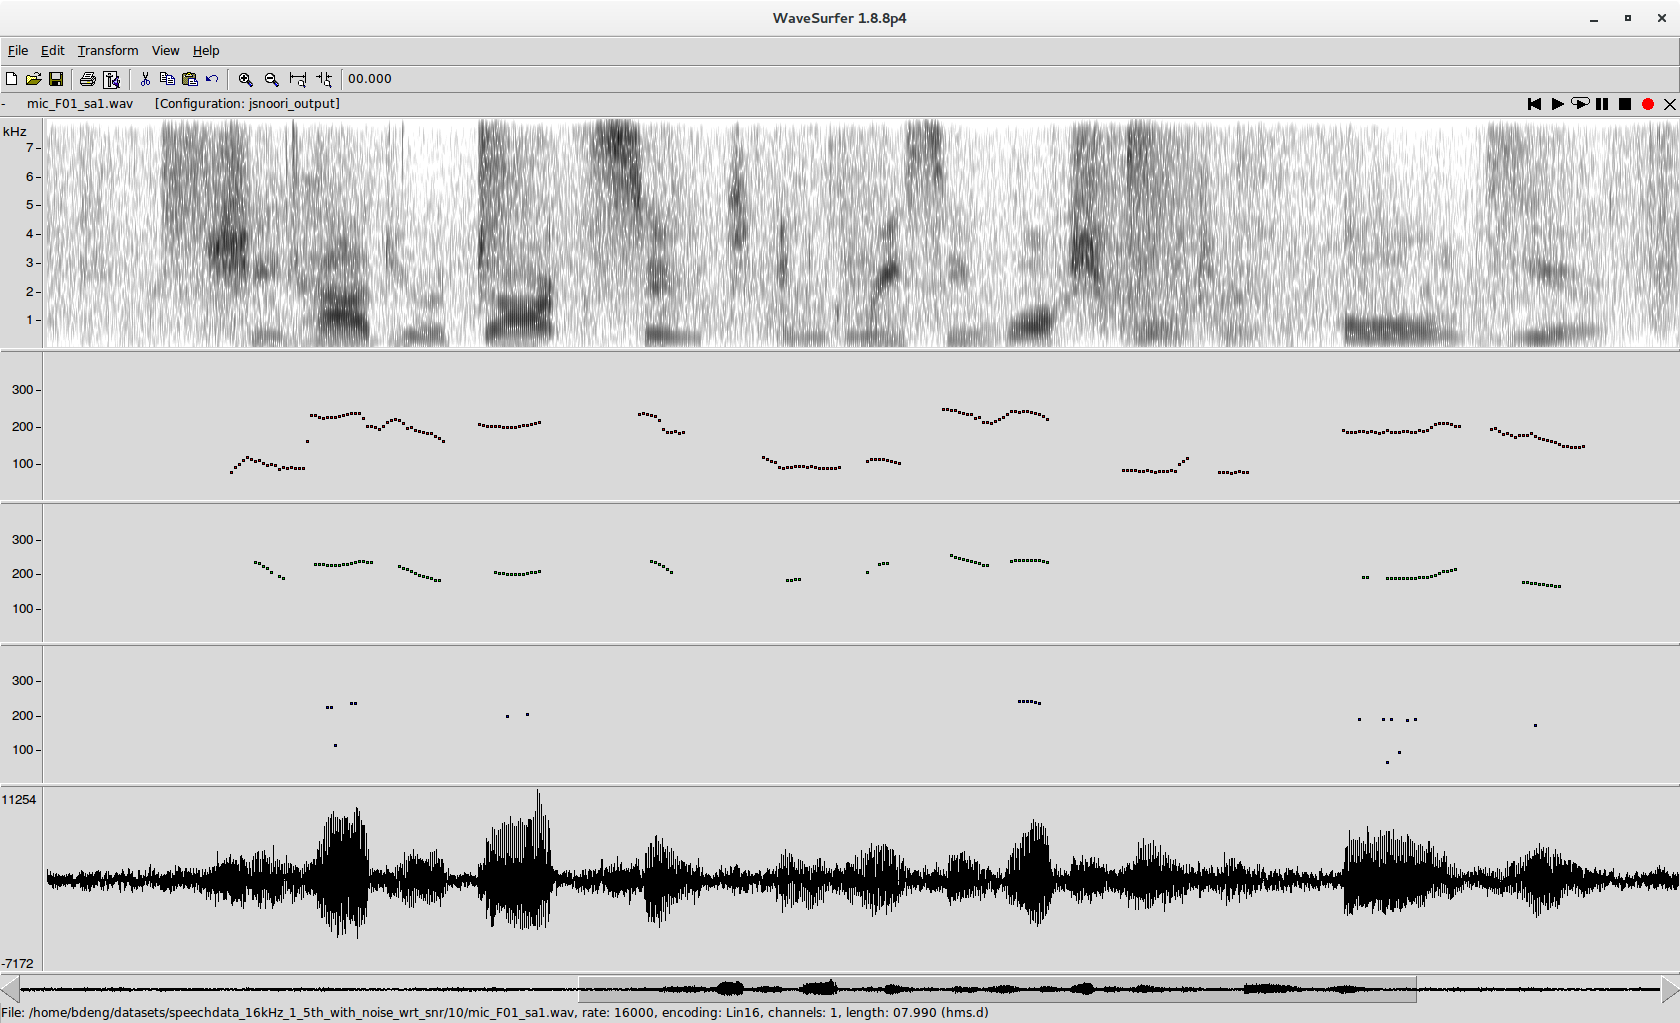
\includegraphics[width=\textwidth]{snr_10dB.png}
    \caption{SNR = \SI{10}{dB}}
    \label{fig:snr-compare-10db}
  \end{subfigure}

  \begin{subfigure}{0.7\textwidth}
    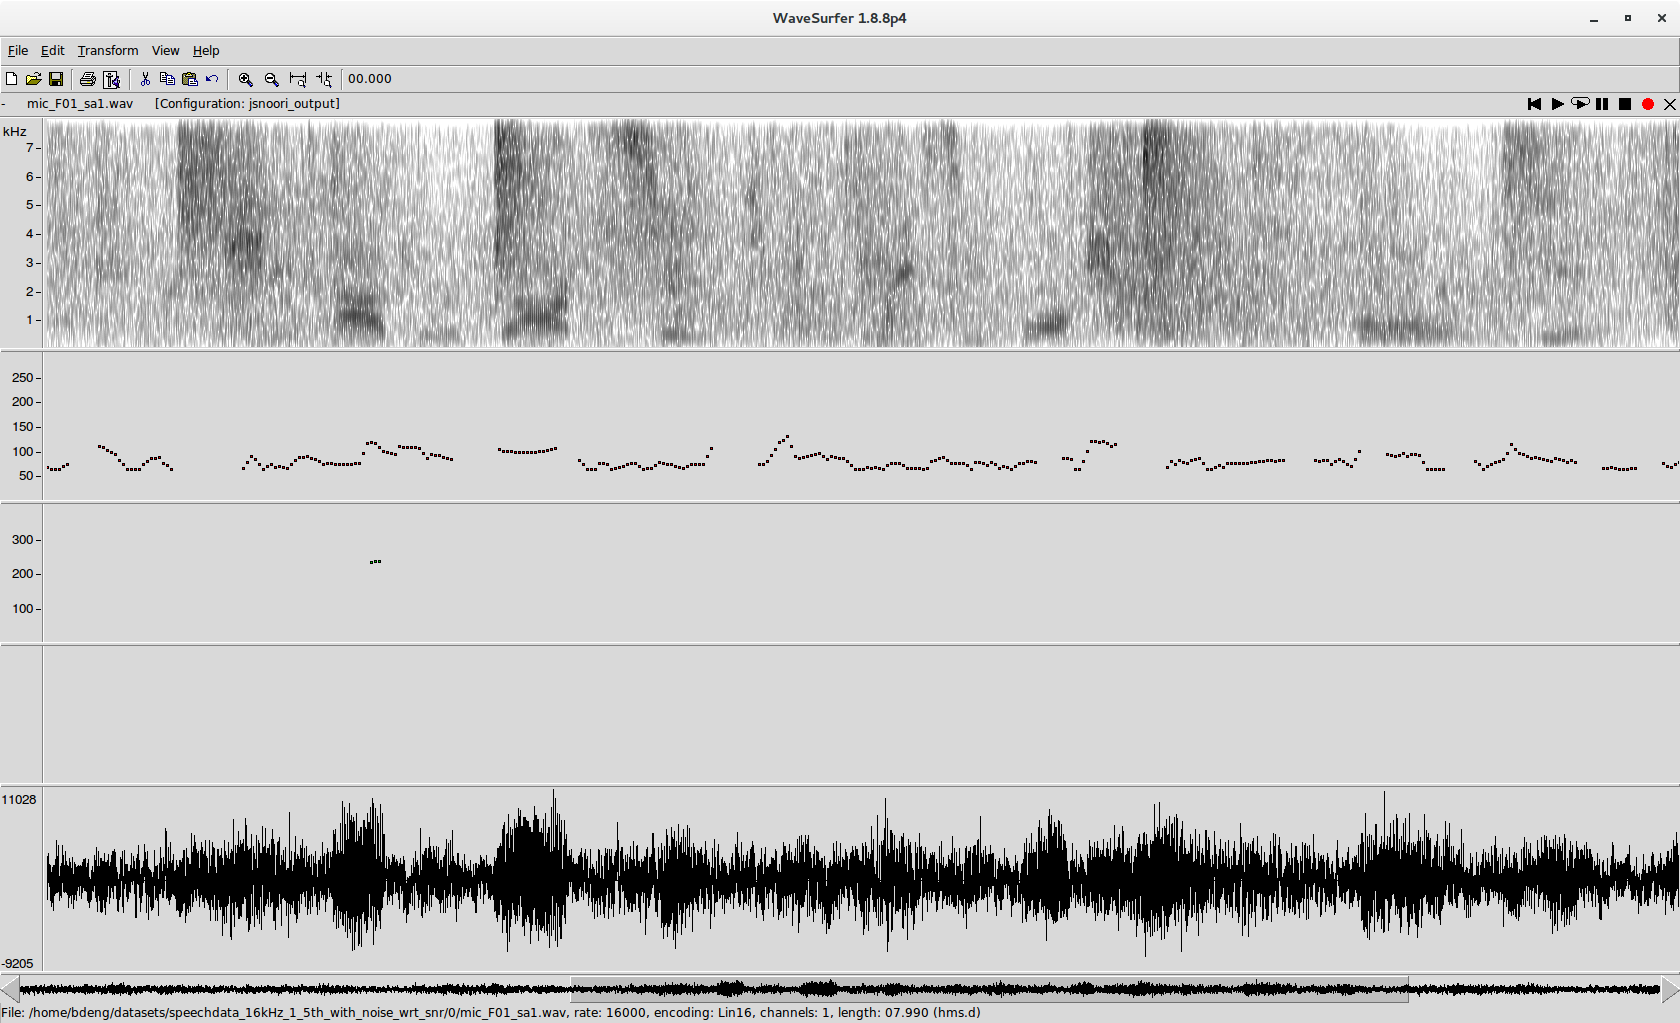
\includegraphics[width=\textwidth]{snr_0dB.png}
    \caption{SNR = \SI{0}{dB}}
    \label{fig:snr-compare-0db}
  \end{subfigure}

  \caption[Visualization of distortions.]{Spectrogram, plot of estimated F0 values, and waveform shown in Wavesurfer.
    From top to bottom, signal-to-noise ratios are \SIlist{20;10;0}{\deci\bel}, respectively.
    When the audio is highly distorted, lots of details in spectrogram and waveform are lost and it's really hard to do fundamental frequency estimation.}
  \label{fig:snr-compare}
\end{figure}

We further distinguish between error types (\autoref{fig:snr-error-types}), which helps us analyze the drawbacks of the algorithms under certain circumstances.
Three types of errors are investigated, namely

\begin{itemize}
  \item \enquote{deviated} (voiced both in reference and result but the result deviates too far from the reference)
  \item \enquote{incorrectly voiced} (unvoiced in reference but voiced in result)
  \item \enquote{incorrectly unvoiced} (voiced in reference but unvoiced in result)
\end{itemize}

\begin{figure}[htbp]
  \centering
  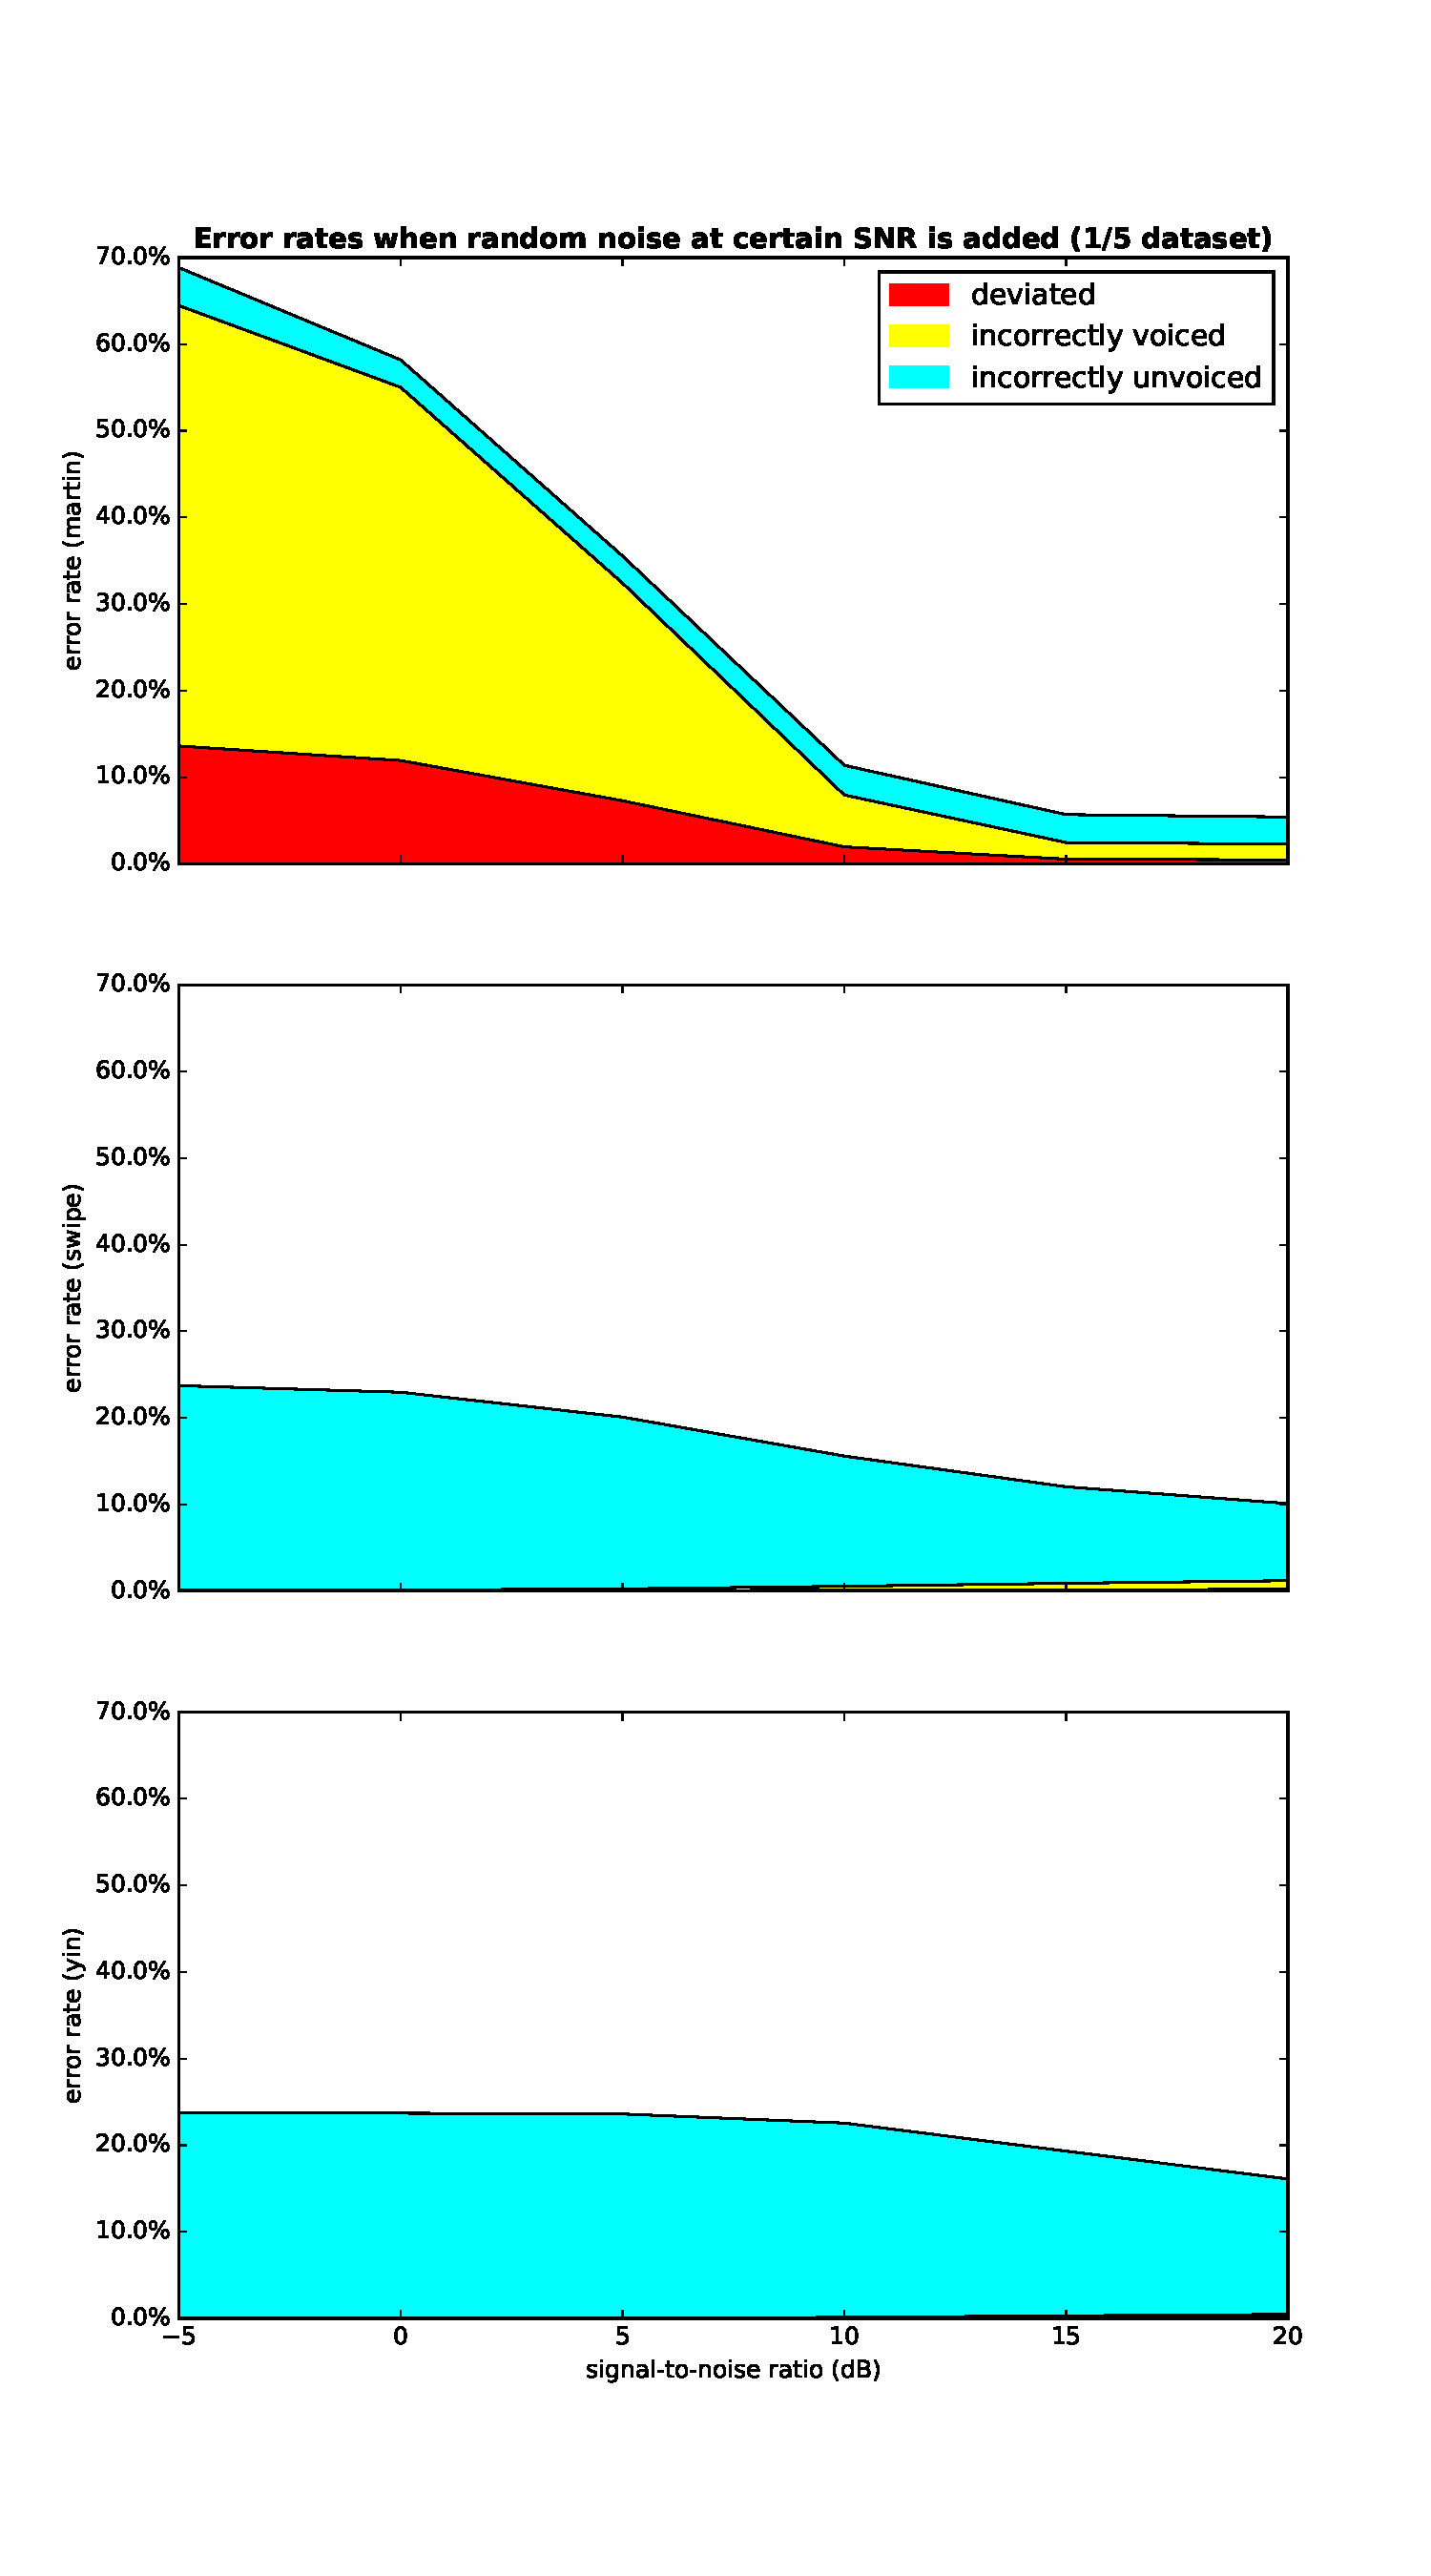
\includegraphics[width=0.8\textwidth]{error_rates_vs_snrs_error_types.pdf}
  \caption{Stack plot of the three error types.} \label{fig:snr-error-types}
\end{figure}

When the signal-to-noise ratio is fixed across different types of noise, it will be easier to investigate the effect of a noise signal's acoustic properties on fundamental frequency estimation.

Next, we sample random noise from the five files separately, \enquote{decomposed} \autoref{fig:random-noise-snr-same-algorithm} and \autoref{fig:random-noise-snr-same-audio} are provided.

\begin{mdframed}
\textbf{Comment and Analysis} (\autoref{fig:snr} and \autoref{fig:snr-error-types})

\bigskip

SWIPE and YIN have virtually only \enquote{incorrectly unvoiced} errors.
When the audio is highly distorted, SWIPE and YIN consider all frames to be unvoiced, while enhanced Martin's algorithm tends to do the opposite and introduce a lot of \enquote{incorrectly voiced} errors.
At the same time, estimation results on voiced frames are more or less acceptable.

\textbf{This phenomenon indicates that a more sophisticated voiced or unvoiced decision mechanism can greatly improve all three algorithms.}
\end{mdframed}

\begin{mdframed}
\textbf{Comment and Analysis} (\autoref{fig:random-noise-snr-same-algorithm} and \autoref{fig:random-noise-snr-same-audio})

From \autoref{fig:random-noise-snr-same-algorithm} we can see that YIN performs badly under white noise, which has the least influence on enhanced Martin's algorithm and SWIPE\@.
After comparing the spectrograms of the five noise types, we conclude that \textbf{YIN is highly sensitive to high-frequency components in the noise}.
\textbf{This makes sense again because YIN is correlation-like.
High-frequency noise totally smoothes the audio signals.}

YIN performs best under \texttt{babble.wav} noise which doesn't have many high-frequency components.
In contrast, the other four do, and most notably in \texttt{factory2.wav} (sounds from cut wheel machines).
\end{mdframed}

\begin{figure}[htbp]
  \centering
  \begin{subfigure}{0.7\textwidth}
    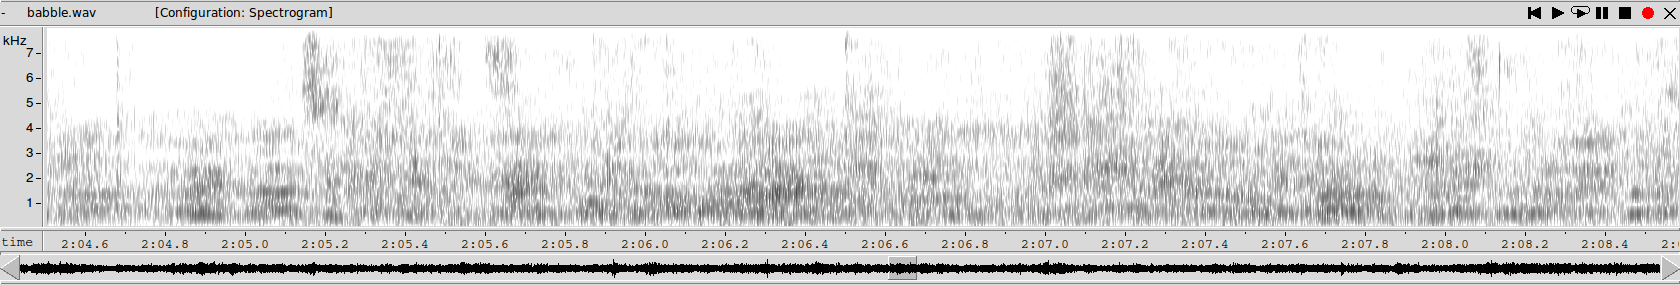
\includegraphics[width=\textwidth]{babble-spectrogram}
    \caption{\texttt{babble.wav}}
    \label{fig:babble-spectrogram}
  \end{subfigure}

  \begin{subfigure}{0.7\textwidth}
    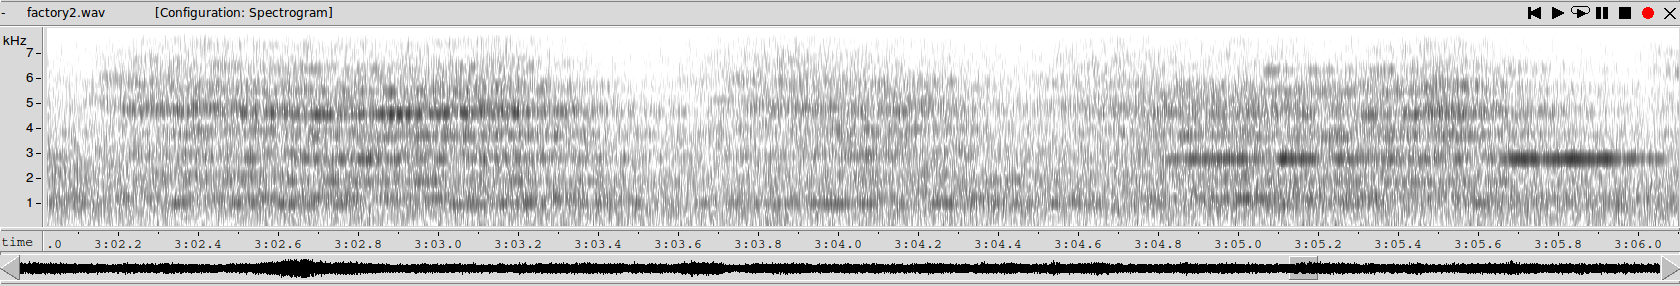
\includegraphics[width=\textwidth]{factory2-spectrogram}
    \caption{\texttt{factory2.wav}}
    \label{fig:factory2-spectrogram}
  \end{subfigure}

  \caption{Spectrograms of \texttt{babble.wav} and \texttt{factory2.wav}.} \label{fig:noise-spectrogram}
\end{figure}

\begin{figure}[htbp]
  \centering
  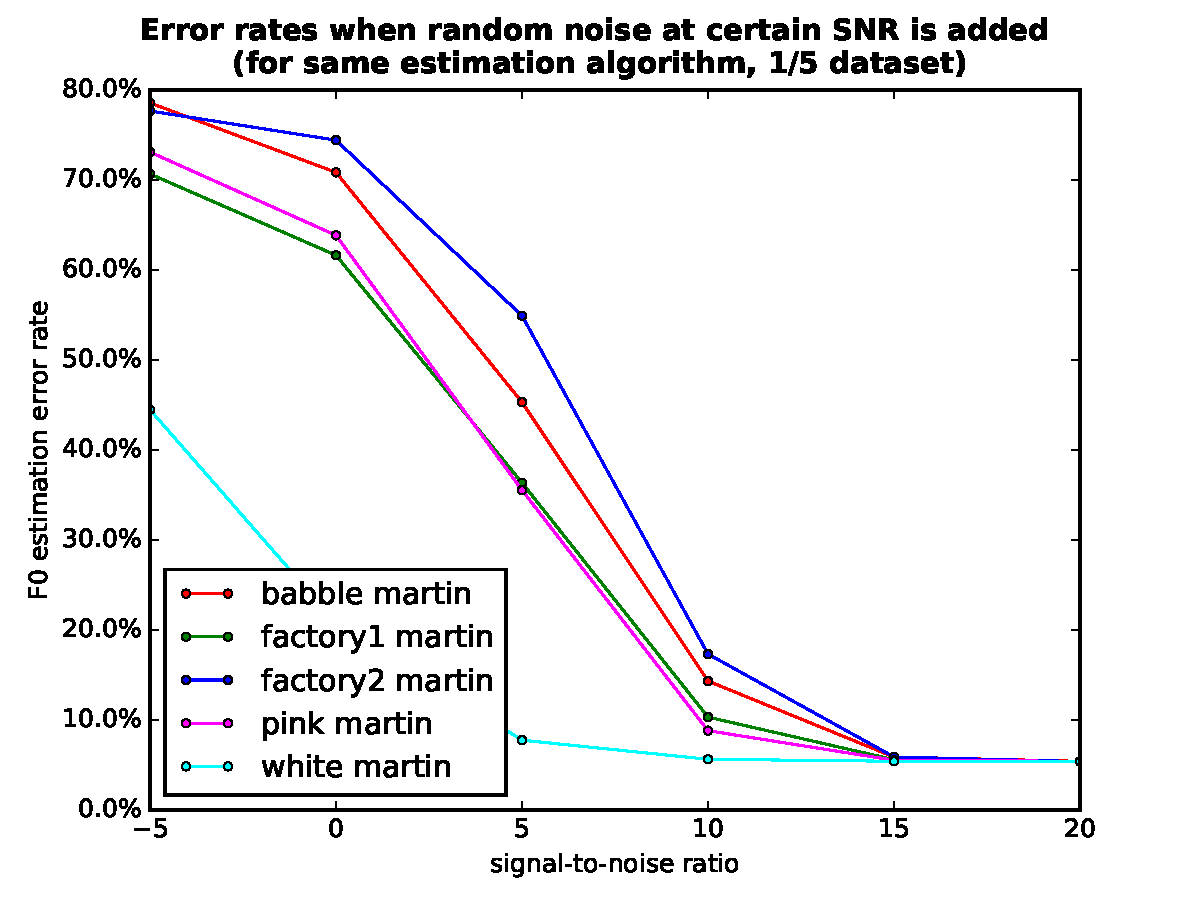
\includegraphics[width=0.65\textwidth]{error_rates_random_noise_wrt_snr_martin.pdf}
  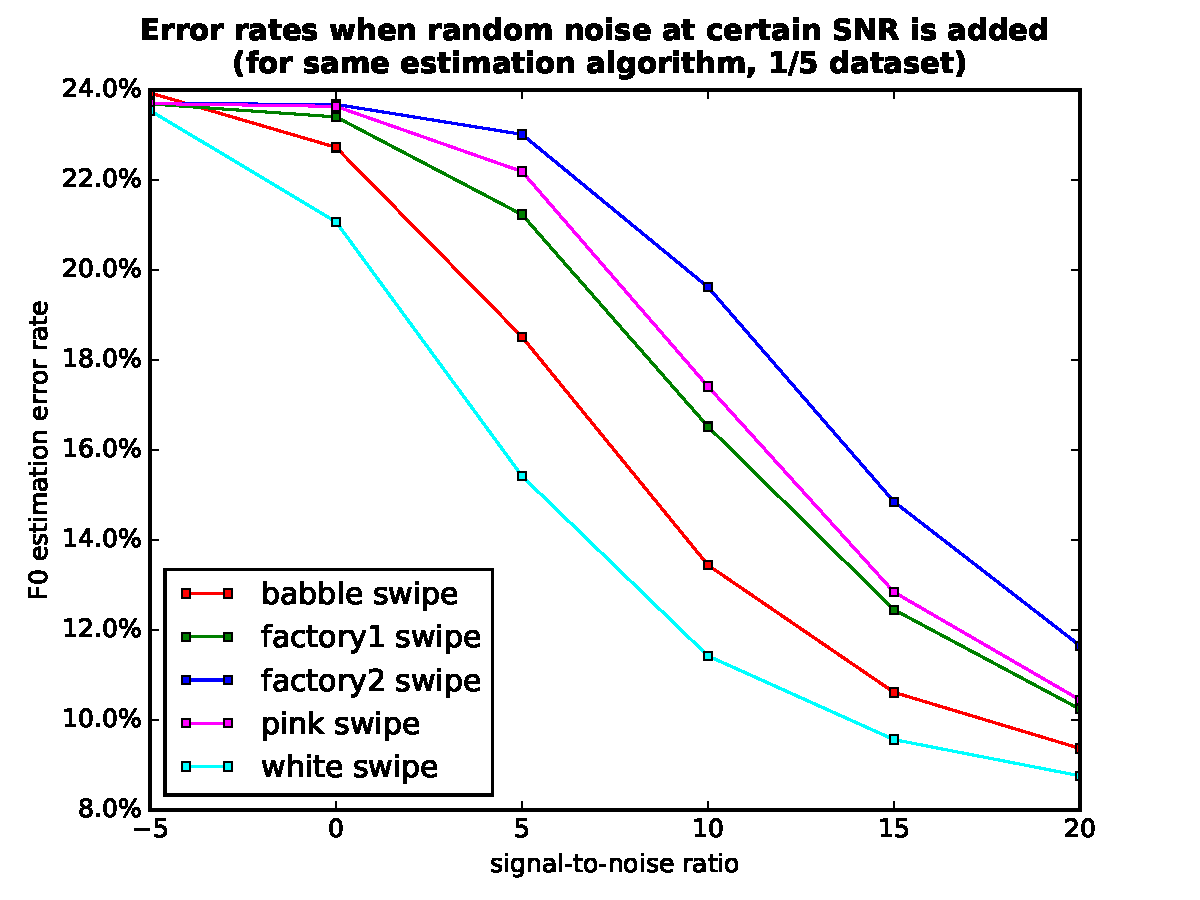
\includegraphics[width=0.65\textwidth]{error_rates_random_noise_wrt_snr_swipe.pdf}
  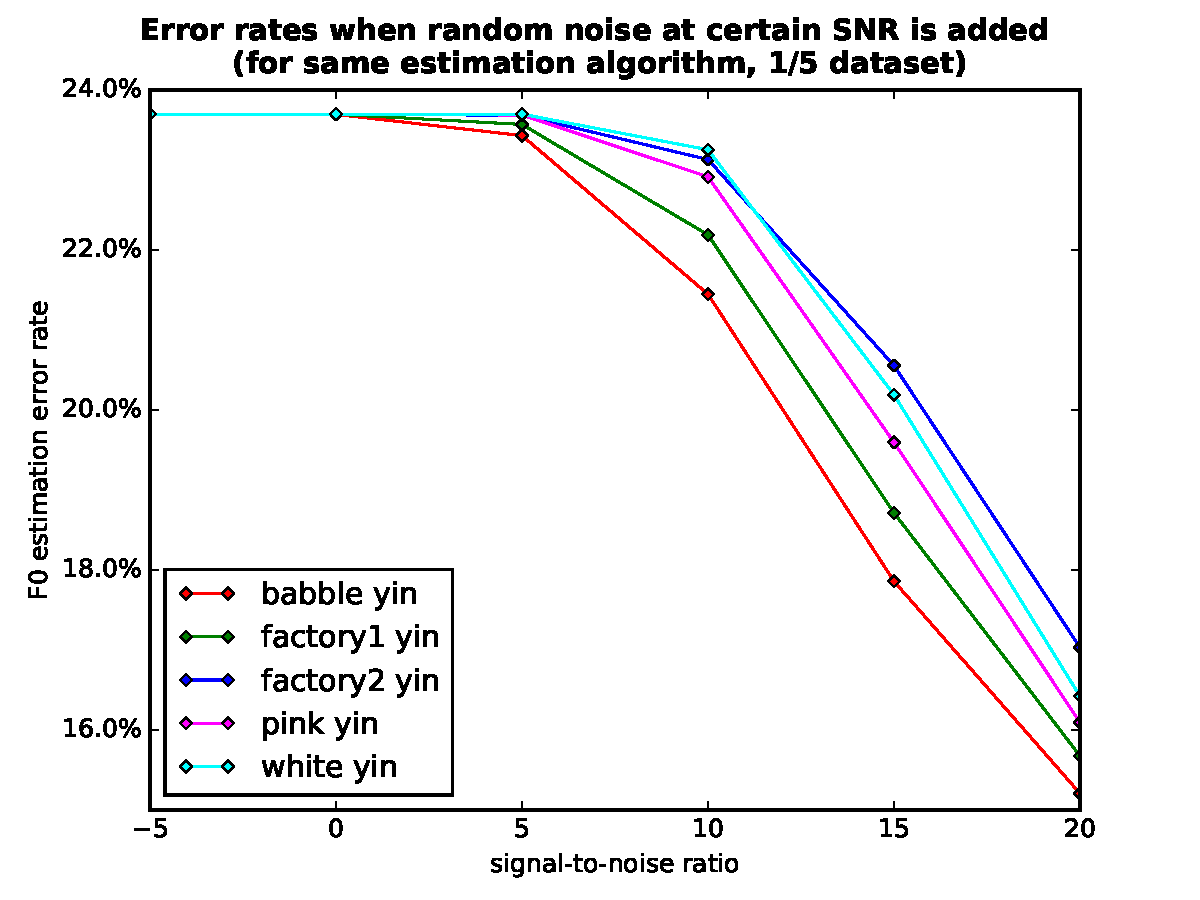
\includegraphics[width=0.65\textwidth]{error_rates_random_noise_wrt_snr_yin.pdf}
  \caption[Error rates of the same algorithm when random noise at certain SNR is sampled from different audios.]{Error rates of the same algorithm when random noise at certain SNR is sampled from different audio signals.
    Subfigures have different y-axis limits.}
  \label{fig:random-noise-snr-same-algorithm}
\end{figure}

\begin{figure}[htbp]
  \centering
  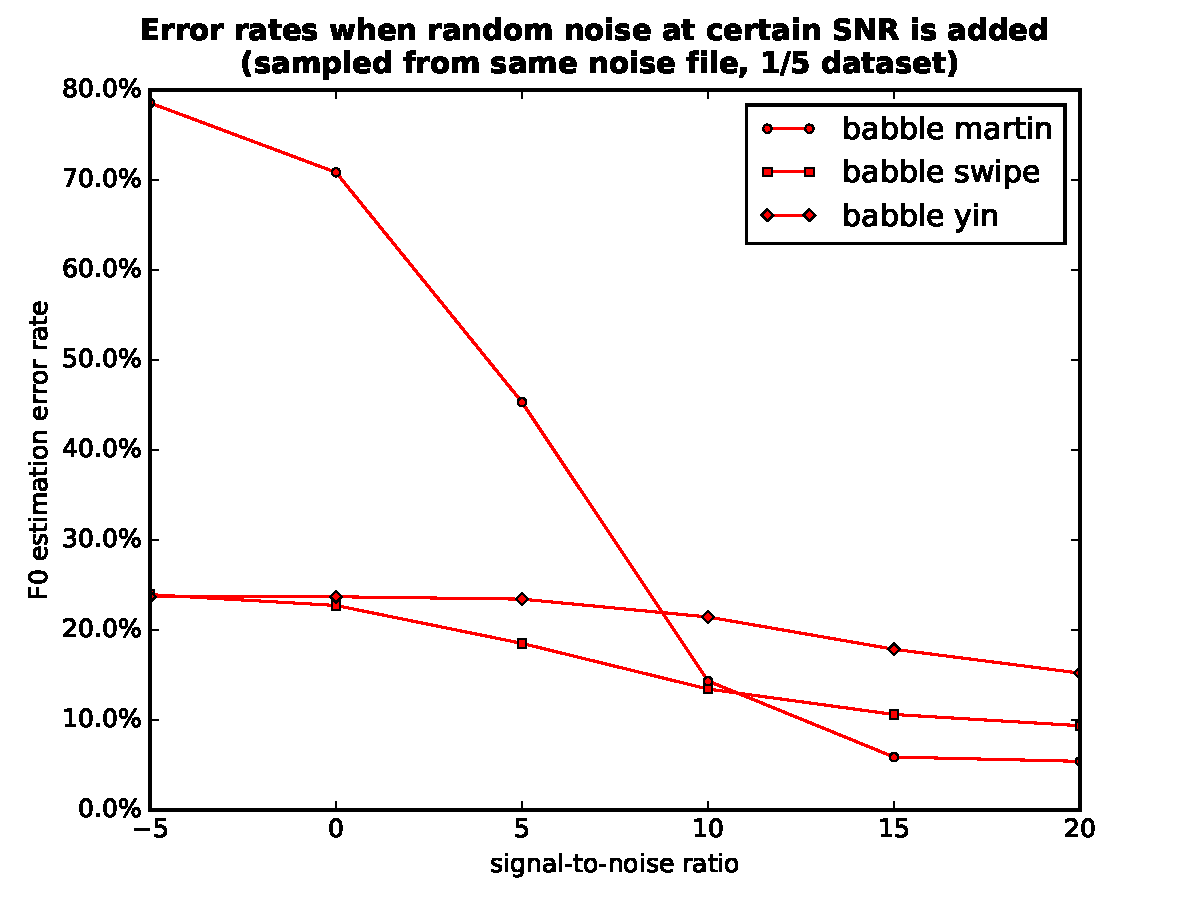
\includegraphics[width=0.49\textwidth]{error_rates_random_noise_wrt_snr_babble.pdf}
  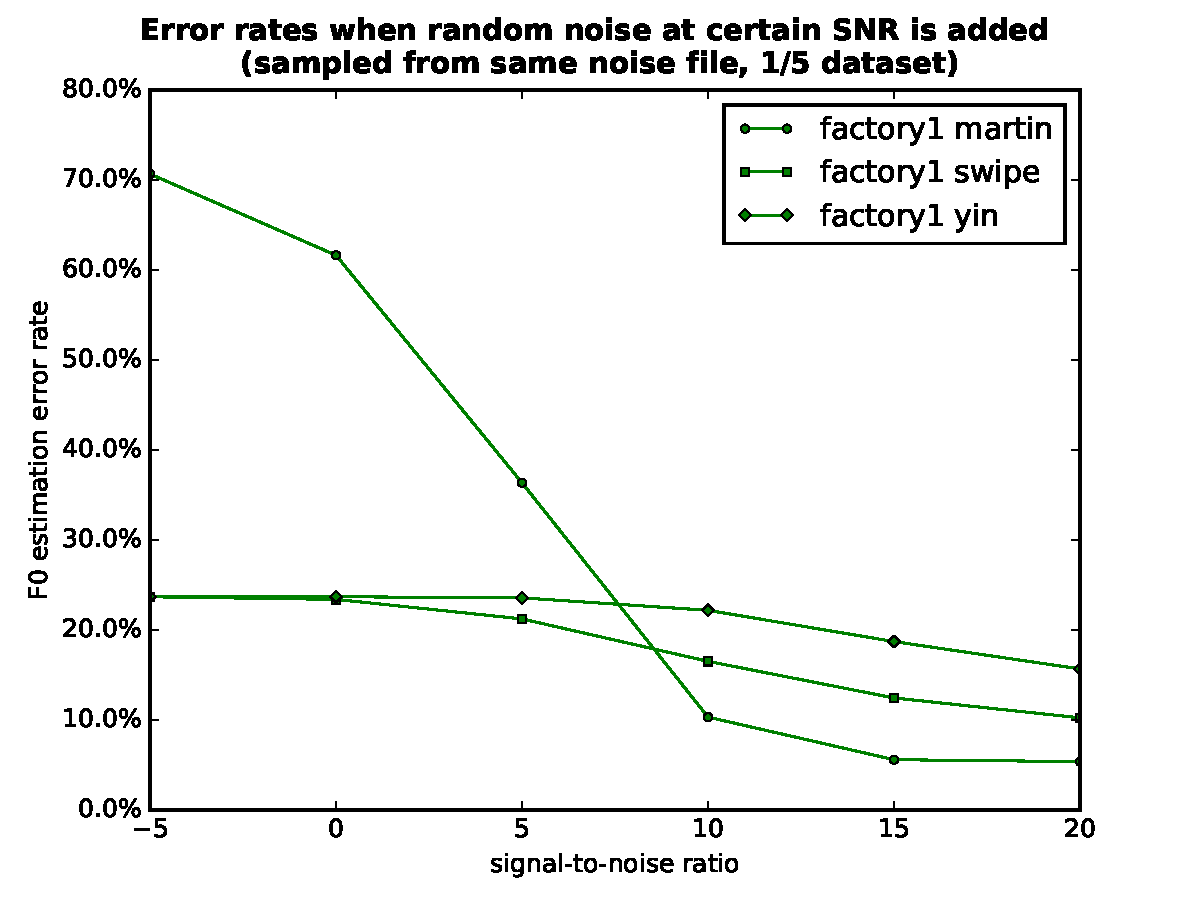
\includegraphics[width=0.49\textwidth]{error_rates_random_noise_wrt_snr_factory1.pdf}
  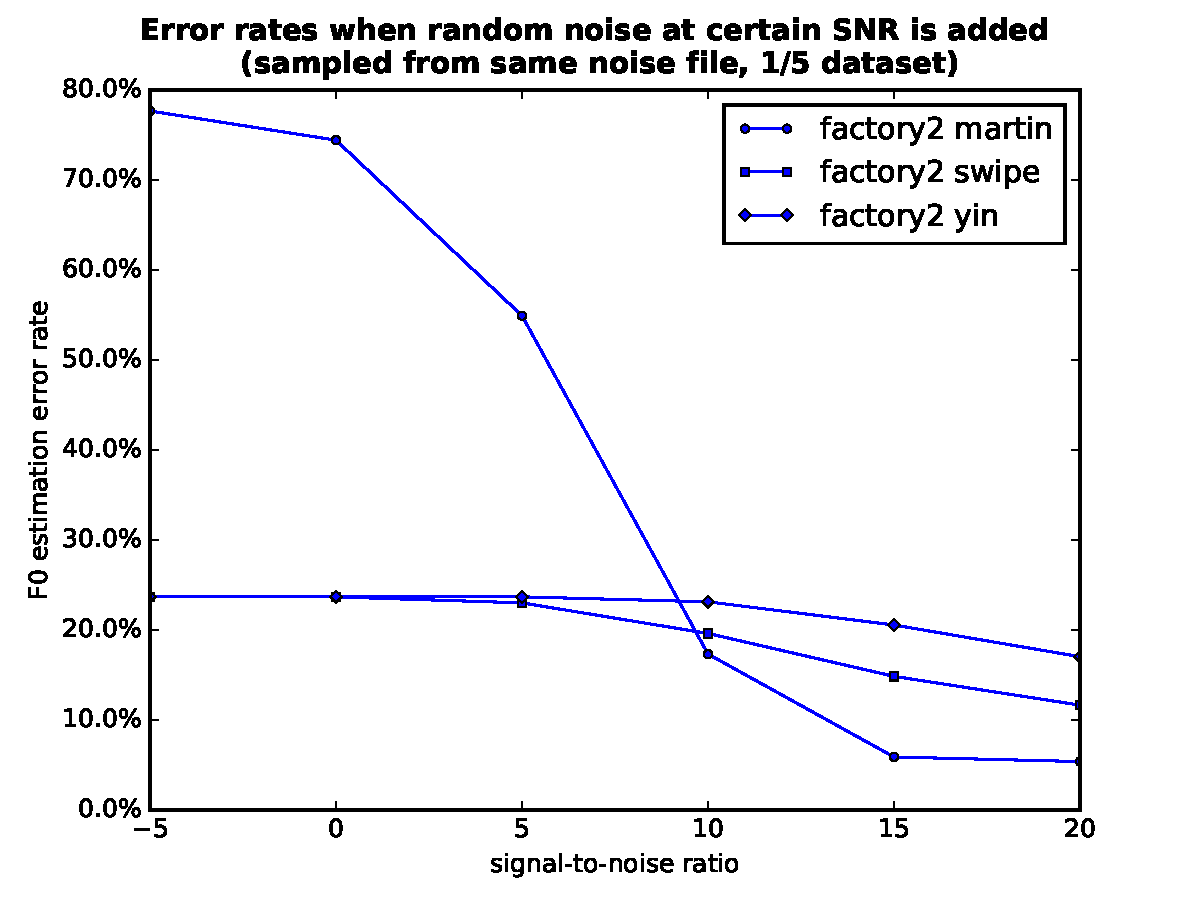
\includegraphics[width=0.49\textwidth]{error_rates_random_noise_wrt_snr_factory2.pdf}
  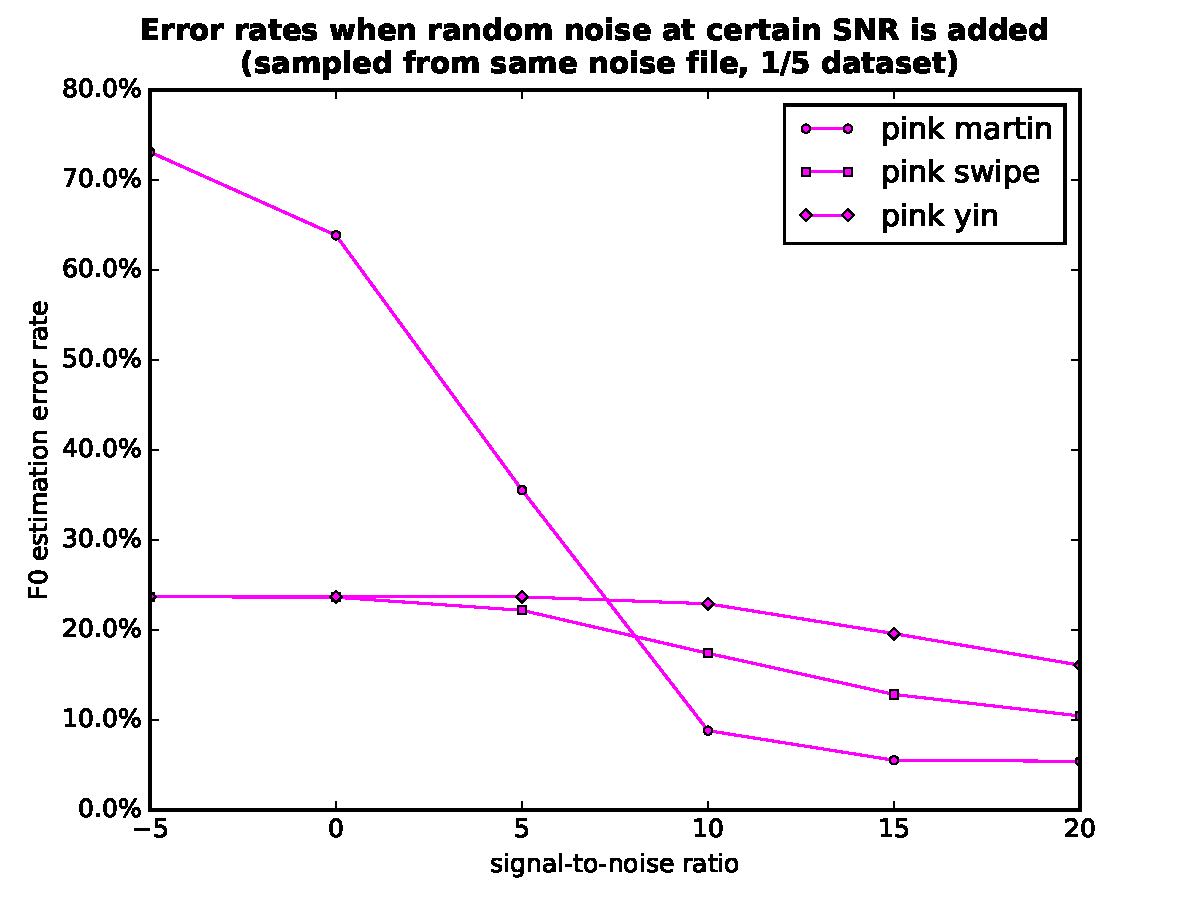
\includegraphics[width=0.49\textwidth]{error_rates_random_noise_wrt_snr_pink.pdf}
  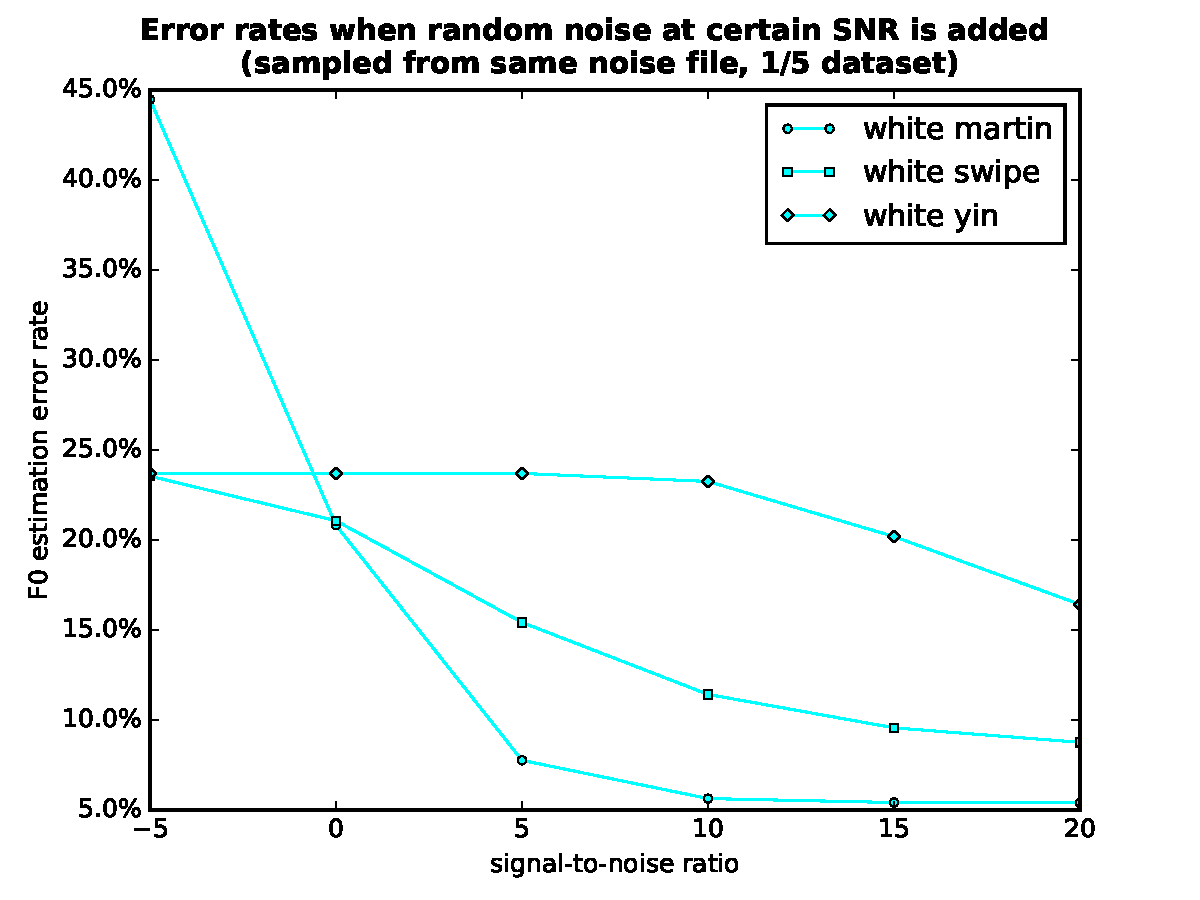
\includegraphics[width=0.49\textwidth]{error_rates_random_noise_wrt_snr_white.pdf}
  \caption[Error rates of different algorithms when random noise at certain SNR is sampled from the same audio.]{Error rates of different algorithms when random noise at certain SNR is sampled from the same audio.
    Subfigures have different y-axis limits.}
  \label{fig:random-noise-snr-same-audio}
\end{figure}

\chapter{Confidence Measures on Fundamental Frequency Estimations}

As we have stated, none of the existing fundamental frequency estimation algorithms provide a confidence measure.

We treat the prediction of correctness of existing algorithms' estimations as a binary classification problem (correct/incorrect) and design neural network classifiers to output a confidence value, based on the theorem introduced above.
Of course, additional information besides estimated fundamental frequency is needed to make the classifiers accurate enough.

\section{Features and labels}

Each run of the fundamental frequency estimation algorithms generates a sample (feature-label pair) for supervised learning and for evaluation.

\begin{mdframed}
\noindent \textbf{Features}:

Various features are used by the classifiers, some of which are intermediate results computed during estimations, in total there are 59 dimensions:

\begin{itemize}
  \item energy of the signal
  \item three ranked candidate results, along with their correlation values
  \item 40 cepstral coefficients and 12 Mel-frequency cepstral coefficients (MFCCs) \parencite{mermelstein1976distance,davis1980comparison}
\end{itemize}

\noindent \textbf{Labels}:

Labels are obtained when calculating error rates during the empirical analyses.
We use 0 for incorrect and 1 for correct.
\end{mdframed}

\newpage

\section{Neural network architectures}

The underlying neural network architectures we designed are multilayer perceptron (MLP) and recurrent models with long short-term memory (LSTM) \parencite{hochreiter1997long} to incorporate information from context while avoiding the problem with long-term dependencies.

\subsection{MLP classifier}

\begin{mdframed}
\noindent \textbf{MLP classifier} (\autoref{fig:mlp-draw}):
\begin{itemize}
  \item two dense layers of hidden units with ReLU \parencite{nair2010rectified} activation function
  \item a single output unit with \texttt{sigmoid} activation
  \item dropout \parencite{srivastava2014dropout} layers to prevent overfitting
\end{itemize}
\end{mdframed}

\begin{figure}[htbp]
  \centering
  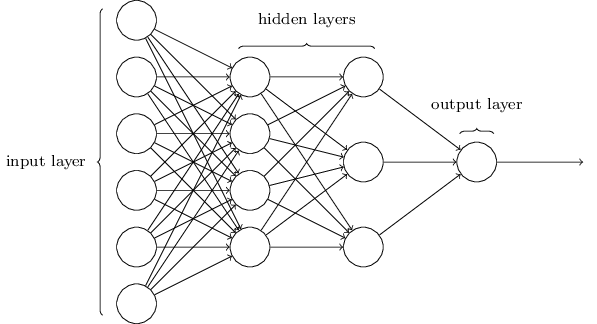
\includegraphics[width=0.8\textwidth]{mlp.png}
  \caption{Diagram of the MLP classifier.} \label{fig:mlp-draw}
\end{figure}

\autoref{fig:mlp} is the computation graph of our MLP classifier, given by the neural network library we use.
Data flow from top to bottom.

Tuples like \texttt{(None, 59)} provide information about each layer:

\begin{itemize}
  \item The first element is the batch size.
    \texttt{None} indicates that any positive integer may be expected.
    But people usually use a power of 2 as batch size so that it is computationally efficient.
  \item The second element is the dimension of input/output variable (for output variable it's also the number of nodes in that layer).
\end{itemize}

\begin{figure}[htbp]
  \centering
  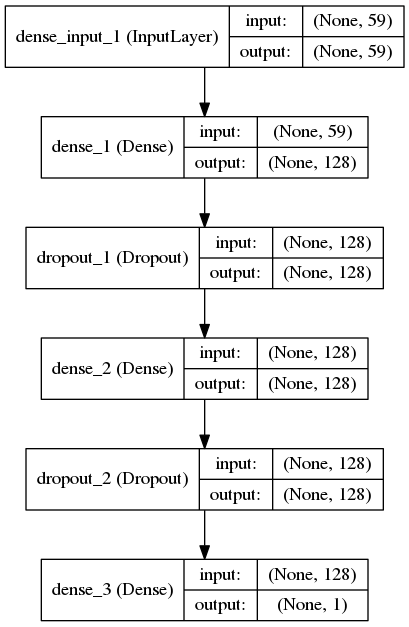
\includegraphics[width=0.7\textwidth]{model-mlp.png}
  \caption{Computation graph of the MLP classifier.} \label{fig:mlp}
\end{figure}

\newpage

\subsection{LSTM classifier}

\begin{mdframed}
\noindent \textbf{LSTM classifier}:
\begin{itemize}
  \item two LSTM recurrent layers which encode temporal information and feed sequences of activation values into the next layers
  \item a dense layer assigns weights to values in the whole sequence
  \item a single output unit with \texttt{sigmoid} activation
  \item dropout \parencite{srivastava2014dropout} layers to prevent overfitting
\end{itemize}
\end{mdframed}

Its computation graph is shown in \autoref{fig:lstm}.

Now the tuples have three elements:

\begin{itemize}
  \item The first element is still the batch size.
  \item The second element is the input sequence length (number of time steps).
    For an input sequence of length \(n\), we think the last sample has temporal dependencies upon samples of the previous \(n-1\) time steps.
    This is a hyperparameter and we try different values of it.
  \item Input/output variable dimension moves to the third position.
\end{itemize}

\begin{figure}[htbp]
  \centering
  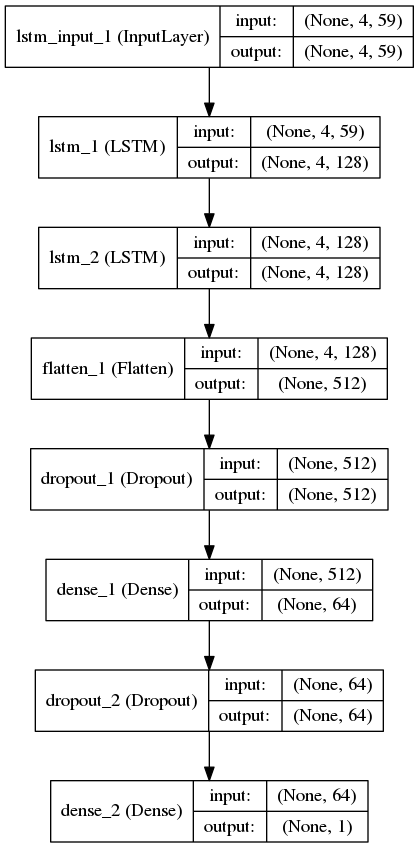
\includegraphics[width=0.7\textwidth]{model-lstm.png}
  \caption{Computation graph of the LSTM classifier.} \label{fig:lstm}
\end{figure}

\newpage

\subsection{Other architectures}

We also investigated other classic architectures for sequence classification, for example, using a max-pooling or average-pooling layer to aggregate the sequence outputs of the LSTM cells, which is popular in the sentiment analysis task.

\begin{figure}[htbp]
  \centering
  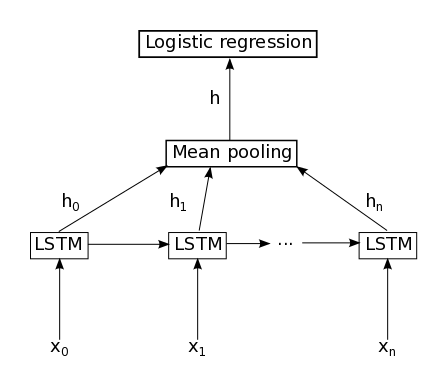
\includegraphics[width=0.6\textwidth]{sentiment.png}
  \caption{Mean-pooling (average-pooling) before output layer.} \label{fig:sentiment}
\end{figure}

But in our experiments, despite prolonged tuning, it never outperforms the MLP model.

The cause might be that neighboring time steps (neighboring estimations in our case) have much more complex patterns of dependency, while equal treatment and simple aggregation won't be able to discover them and actually hides the information from upcoming layers.

\chapter{Experiments}

\section{Data preparation}

The fundamental frequency estimation algorithms have relatively low error rates on clean signals.
If we train only on the original dataset, the resulting classifiers would be biased because of lack of negative samples.

So during training and testing, distorted audio files obtained during the empirical analyses (signal-to-noise ratio at \SI{-5}{\deci\bel}) are used in addition to the original dataset to balance the number of positive and negative samples.
In total, there are approximately 7 million samples for each fundamental frequency estimation algorithm.

\bigskip

After preprocessing, they are stored in matrix-like data structures where each row is a sample.
An auxiliary index indicates which audio file they come from.
Within the same audio file, samples are sorted in chronological order.
This will be useful if we want to explore temporal dependencies.

\begin{figure}[htbp]
  \centering
  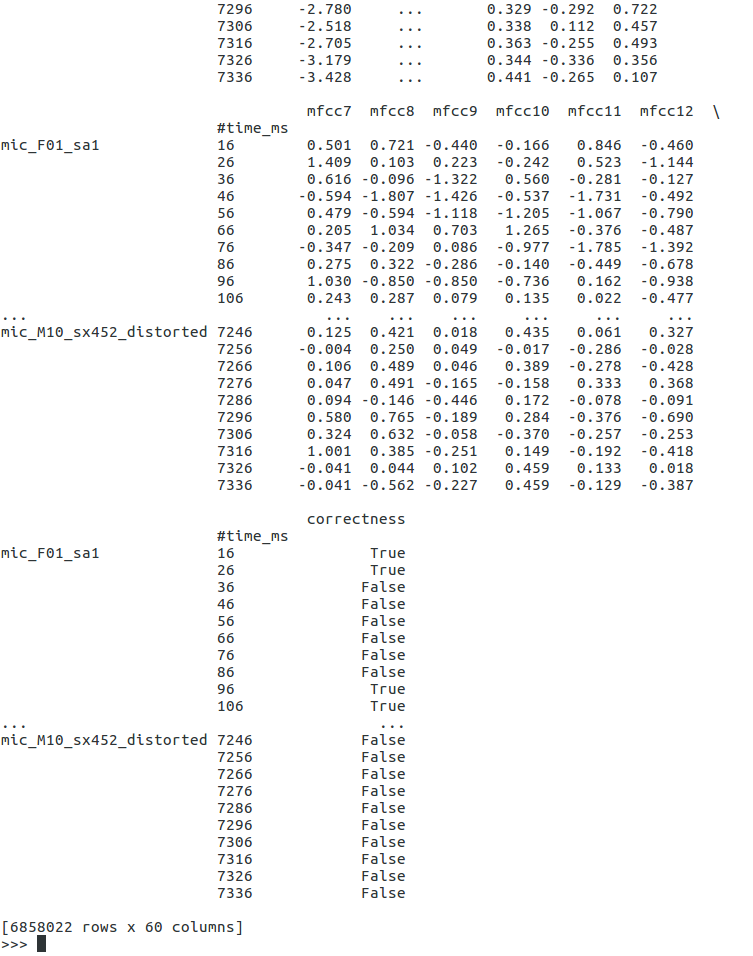
\includegraphics[width=0.55\textwidth]{df.png}
  \caption[Data storage scheme.]{A very small part of the \texttt{pandas} DataFrame storing our data for Martin's algorithm.
    There are in total 60 columns (59-dimensional features plus one-dimensional label).
    The two-level hierarchical indexing consists of audio file basename and time offsets within the audio file.
    Audio files with additive noises have a \enquote{\texttt{\_distorted}} suffix.}
  \label{fig:df}
\end{figure}

Then the dataset is split into training and testing sets (\SIrange[range-phrase=/]{80}{20}{\percent}).

\begin{itemize}
  \item MLP classifier: random sampling on all rows, so the samples are shuffled.
  \item LSTM classifier: in order to maintain the temporal order of samples and avoid constructing invalid sequences across the boundaries of audio files, the split is done on the audio file level.
    Rows from the first \SI{80}{\percent} audio files are taken out as a whole as the training set.

    Then, within each audio file, iterate through the rows and construct \enquote{sequential data} by prepending samples of the past time steps.
    Length of the sequences is a hyperparameter, as we have stated.
\end{itemize}

Furthermore, the last \SI{20}{\percent} of the training set are taken out and used as the validation set.

\section{Training}

The models are trained using stochastic gradient descent (SGD) on mini-batches with binary cross-entropy as objective function.
Class probability threshold for classification is set to 0.5 consistently.

Various techniques from \parencite{lecun2012efficient} and \parencite{orr2003neural} are applied, though nowadays they are becoming standard procedures.

\begin{itemize}
  \item normalize the training data to zero mean, unit variance on each dimension
  \item learning rate decay
  \item Nesterov momentum \parencite{nesterov1983method}
  \item L1 or L2 regularization on the weights
  \item early-stopping using the validation set (if the performance on validation set drops after an epoch, stop updating the parameters immediately)
\end{itemize}

The training takes several hours, up to half a day for each model and hyperparameter setting.

\section{Testing}

When normalizing the training data to zero mean, unit variance on each dimension, we remove the mean value of each feature, then scale by dividing non-constant features by their standard deviation.

The resulting scaler, determined by such mean values and standard deviations calculated on each dimension, must be applied to testing data or new data in production use before feeding them into the models.

\bigskip

\textbf{In this way, the very important assumption in machine learning that training and testing data are sampled from the same distribution still holds, because the same transformation is applied.}

\bigskip

After transformation, the test data is fed into the models with the same batch sizes as during training.
The outputs will be used for evaluation of the models.

\chapter{Results and Evaluation}

We evaluate the performance of the classifiers trained on every algorithm's data by

\begin{itemize}
  \item test accuracy
  \item area under the receiver operating characteristic curve (ROC AUC)
  \item normalized mutual information (NMI)
\end{itemize}

\begin{mdframed}
\textbf{What needs to be clarified is that performance of the classifiers reflects qualities of the generated confidence measures, they are not necessarily related to performance of the fundamental frequency estimation algorithms.}
\end{mdframed}

\section{Metrics}

There are four possible outcomes from a binary classifier, identified by comparing predicted results with ground truth.

\begin{itemize}
  \item true positive, predicted as positive and actually positive
  \item false positive, predicted as positive but actually negative
  \item false negative, predicted as negative but actually positive
  \item true negative, predicted as negative and actually negative
\end{itemize}

We use \(tp\), \(fp\), \(fn\), \(tn\) to denote the number of samples in corresponding categories respectively.
Other metrics are constructed based on these values.

\subsection{Test accuracy}

Test accuracy is the overall accuracy over the testing set.

\begin{equation*}
  accuracy = \frac{tp+tn}{tp+fp+fn+tn}
\end{equation*}

The ideal value is 1.

In our binary classification problem, \enquote{positive} means \enquote{fundamental frequency estimation result is correct} and \enquote{negative} means \enquote{fundamental frequency estimation result is incorrect}.

During the calculation of this metric, class probability thresholds are set to 0.5 for both classes, which means if the \texttt{sigmoid} activation value is greater than 0.5 then sample is classified as \enquote{positive}, otherwise \enquote{negative}.

\subsection{Receiver operating characteristic curve}

\begin{figure}[htbp]
  \centering
  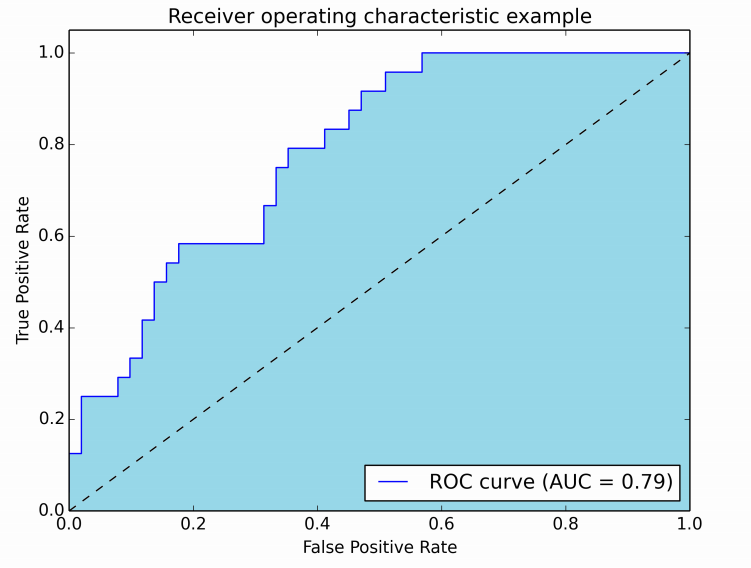
\includegraphics[width=0.8\textwidth]{roc-auc.png}
  \caption{Example ROC curve and its AUC.} \label{fig:roc}
\end{figure}

The receiver operating characteristic (ROC) curve plots true positive rates versus false positive rates for a classifier capable of outputting class probabilities results.

\begin{align*}
  true\ positive\ rate (tpr) & = \frac{tp}{tp+fn} \\
  false\ positive\ rate (fpr) & = \frac{fp}{fp+tn}
\end{align*}

Points on the ROC curve are obtained by setting different thresholds on class probabilities when making classification decisions (instead of fixing them at 0.5).
For example, a classifier outputs 0.7 for being positive and 0.3 for being negative on a certain sample.
If the threshold of positive class's probability is 0.6, then the sample is classified as positive.
While the result will be negative if the threshold rises to 0.8.

Area under the ROC curve can be interpreted as the probability that the classifier will assign a higher score to a randomly chosen positive sample than to a randomly chosen negative sample.
The ideal value is also 1.
In reality, only a finite number of points on the curve can be obtained, so we construct trapezoids under the curve as an approximation to area.

\textbf{As our confidence measures are equal to the positive class probabilities, area under the ROC curve reflects objectively their performance over the whole value range (\numrange{0}{1}).}

\subsection{Normalized mutual information}

Normalized mutual information (NMI) measures agreement of class assignments.

The entropy of a discrete random variable \(X\) is defined as

\begin{equation*}
  H(X) = - \sum_{x \in X} P(x) \log P(x).
\end{equation*}

The mutual information of two discrete random variables \(X\) and \(Y\), measuring mutual dependence, is defined as

\begin{equation*}
  I(X;Y) = \sum_{y \in Y} \sum_{x \in X} P(x,y) \log \left(\frac{P(x,y)}{P(x)P(y)}\right).
\end{equation*}

NMI is obtained by dividing mutual information by the geometric mean of two random variables' entropies.
Its range is between 0 and 1 and again 1 is ideal.

\begin{equation*}
  \mathrm{NMI} = \frac{I(X;Y)}{\sqrt{H(X)H(Y)}}
\end{equation*}

Both the classification results and ground truth can be seen as discrete random variables with possible values \(\lbrace 0,1 \rbrace\) and a probability mass function \(P\).
Then NMI can be applied.
This metric is furthermore symmetric.
So it doesn't matter which one of the two \(X\) and \(Y\) represent.

\newpage

\section{Input sequence length for LSTM model}

During our experimentation, a longer input sequence length (more time steps) in LSTM model gives better results, as shown in \autoref{tab:lstm-isl}.

\begin{table}[htbp]
  \centering
  \begin{tabular}{llSSS}
  	\toprule
  	Model                                      & Tuned for & {Accuracy} & {ROC-AUC} & {NMI} \\
  	\midrule
  	\multirow{3}{*}{LSTM (sequence length: 2)} & Martin's  & 0.926      & 0.968     & 0.641 \\
  	                                           & SWIPE     & 0.880      & 0.870     & 0.219 \\
  	                                           & YIN       & 0.893      & 0.874     & 0.230 \\
  	\midrule
  	\multirow{3}{*}{LSTM (sequence length: 3)} & Martin's  & 0.932      & 0.971     & 0.659 \\
  	                                           & SWIPE     & 0.883      & 0.878     & 0.238 \\
  	                                           & YIN       & 0.901      & 0.889     & 0.272 \\
  	\midrule
  	\multirow{3}{*}{LSTM (sequence length: 4)} & Martin's  & 0.934      & 0.971     & 0.666 \\
  	                                           & SWIPE     & 0.886      & 0.880     & 0.247 \\
  	                                           & YIN       & 0.902      & 0.892     & 0.276 \\
  	\bottomrule
  \end{tabular}
  \caption{Performance of the LSTM model when different input sequence lengths are applied during training and testing.} \label{tab:lstm-isl}
\end{table}

Each line in the table gives the model's classification performance when trained on one of the fundamental frequency estimation algorithms' data.

\bigskip

The increasing performance proves that there are indeed long-term dependencies and our LSTM model is capable of capturing them.
\textbf{It may not be monotonically increasing when the input sequence length grows even longer.}

\newpage

\section{MLP model versus LSTM model}

\autoref{tab:metrics} reports best results for both neural network architectures until now.
They are achieved when there are 128 nodes in both the MLP model's hidden layers and the LSTM model's recurrent layers.
The dense layer in the LSTM model has 64 nodes.
Dropout rate is set to 0.5 uniformly.

\begin{table}[htbp]
  \centering
  \begin{tabular}{llSSS}
  	\toprule
  	Model                                      & Tuned for & {Accuracy} & {ROC-AUC} & {NMI} \\
  	\midrule
  	\multirow{3}{*}{MLP}                       & Martin's  & 0.916      & 0.957     & 0.585 \\
  	                                           & SWIPE     & 0.874      & 0.867     & 0.209 \\
  	                                           & YIN       & 0.863      & 0.829     & 0.143 \\
  	\midrule
  	\multirow{3}{*}{LSTM (sequence length: 4)} & Martin's  & 0.934      & 0.971     & 0.666 \\
  	                                           & SWIPE     & 0.886      & 0.880     & 0.247 \\
  	                                           & YIN       & 0.902      & 0.892     & 0.276 \\
  	\bottomrule
  \end{tabular}
  \caption{Metrics of the best-performing classifiers.} \label{tab:metrics}
\end{table}

\begin{itemize}
  \item Our LSTM model outperforms the MLP model everywhere as expected.
    This shows the advantage of recurrent neural networks.
  \item High accuracy and ROC-AUC values guarantee that our models will be highly applicable in production use.
  \item There are no baselines to compare with.

  \bigskip

  \item NMI results indicate that there is still margin for improvement regarding class assignment.
    A certain type of error is \enquote{dominating} in spite of reference labels.
    It may just be \enquote{incorrectly voiced} error for enhanced Martin's algorithm and \enquote{incorrectly unvoiced} error for SWIPE and YIN.
  \item For now, our models are universal for any fundamental frequency estimation algorithm.
    Special settings for certain algorithms, for example, a simple decision tree based on signal energy will detect SWIPE and YIN's \enquote{incorrectly unvoiced} errors, and thus help improve performance.
    But at the same time we need to make sure the overall classifiers still estimate Bayesian probabilities.
\end{itemize}

\newpage

\section{Performance on distorted audio signals}

To further investigate robustness of our models, the distorted audio corpus at different signal-to-noise ratios are used as extra testing data.

\section{Performance on voiced and unvoiced segments}

Samples can be categorized into voiced and unvoiced segments, based on whether the reference fundamental frequency is greater than zero or not.

The three metrics are then calculated on voiced and unvoiced segments separately. Results are shown in \autoref{fig:distorted-testing-data-accuracy}, \autoref{fig:distorted-testing-data-roc-auc} and \autoref{fig:distorted-testing-data--nmi}.

\begin{itemize}
  \item Generally speaking, our classifiers work better on unvoiced segments. One possible explanation is that the feature space is much smaller for unvoiced segments, so it's easier for a classifier to generalize.
  \item LSTM model outperforms MLP model on voiced segments, which confirms again the existence of temporal dependencies in our problem.
  \item Non-mononicity in the curves indicates fluctuation in the size of feature space. The classification problem is most difficult when there is a moderate amount of noise.
  \item Training on data at certain signal-to-noise ratio might be necessary depending on use cases.
\end{itemize}

\begin{figure}[htbp]
  \centering
  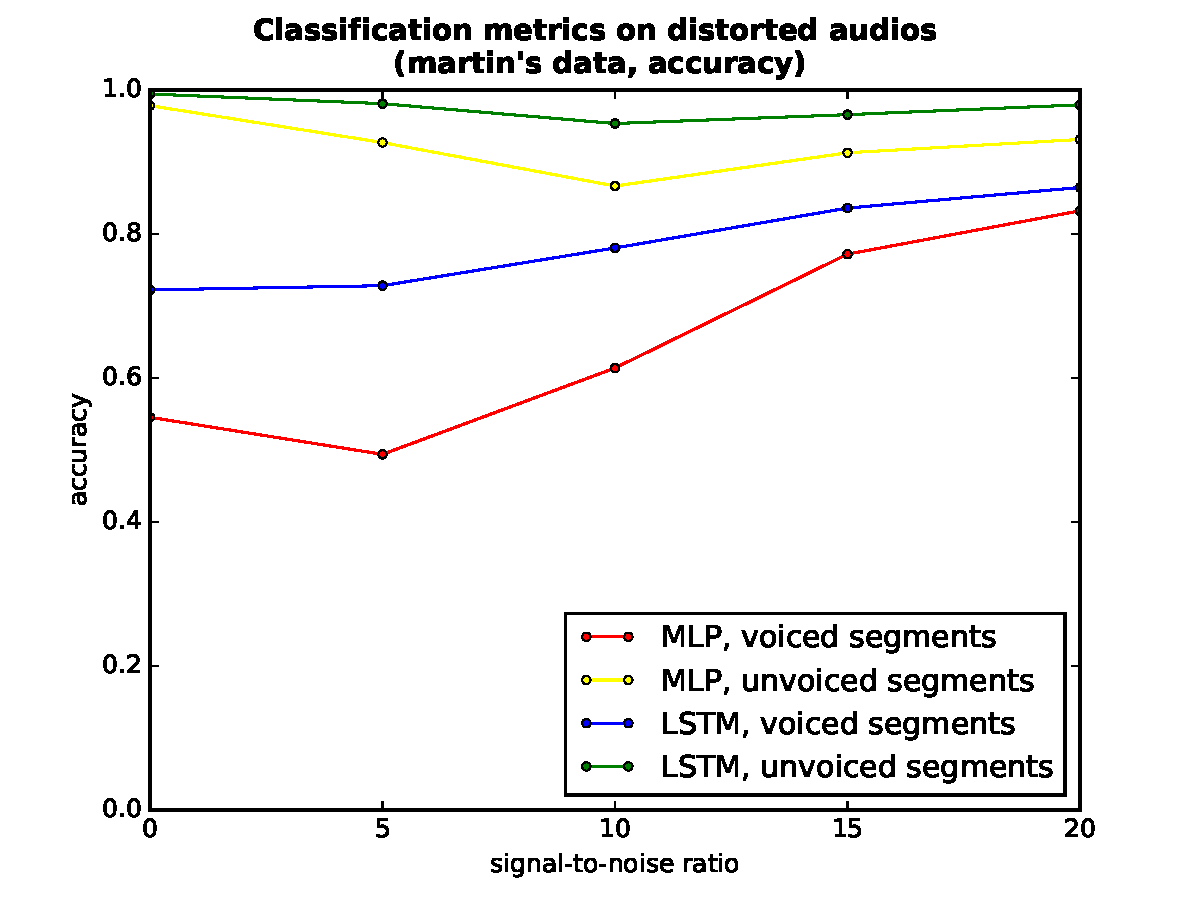
\includegraphics[width=0.65\textwidth]{classification_metrics_martin_accuracy.pdf}
  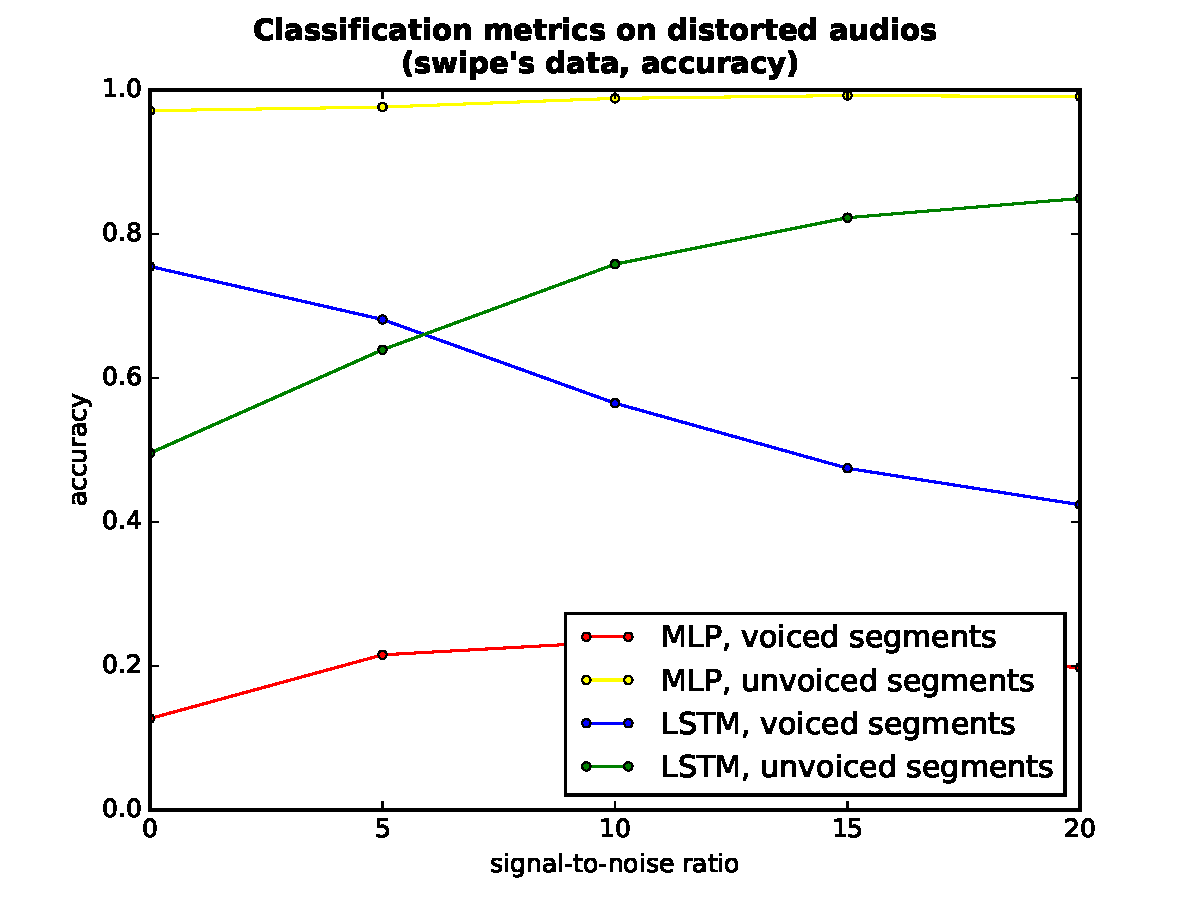
\includegraphics[width=0.65\textwidth]{classification_metrics_swipe_accuracy.pdf}
  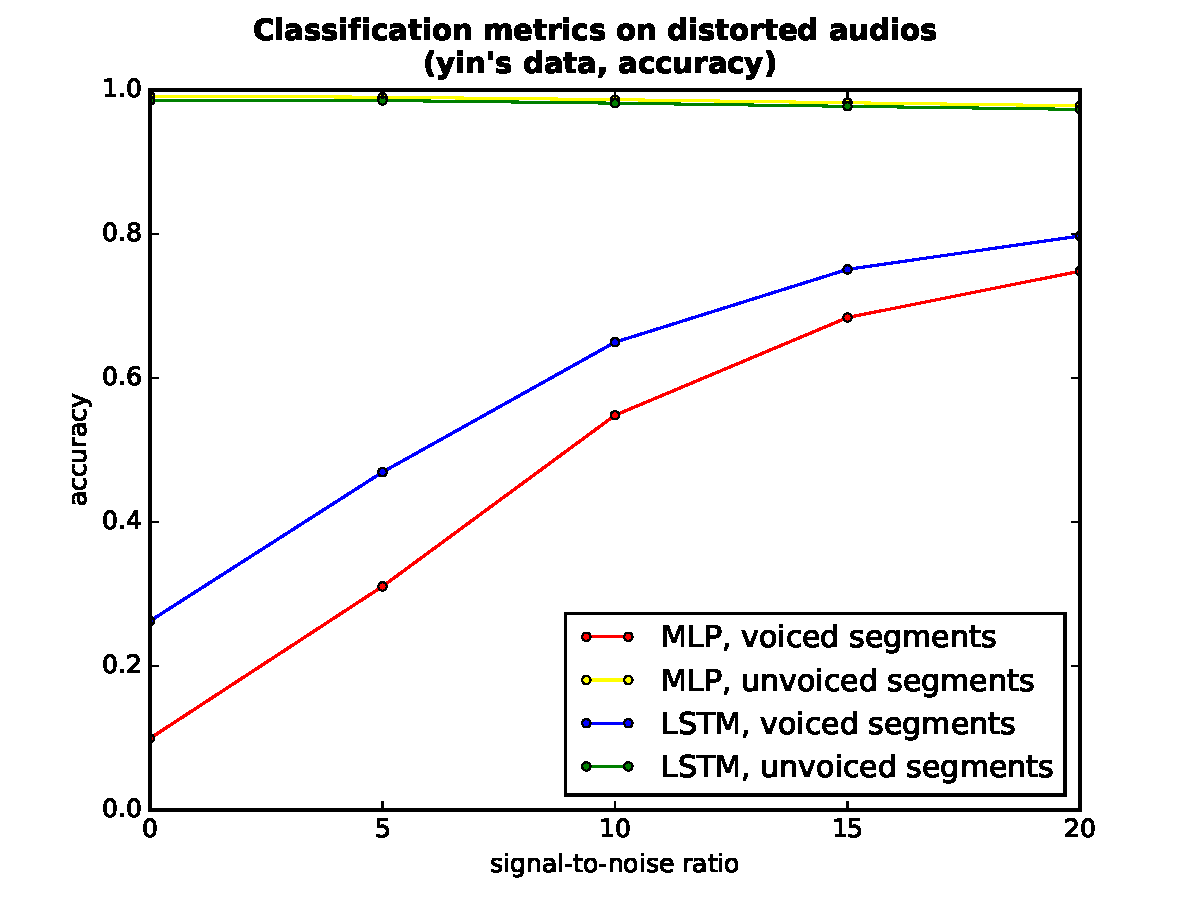
\includegraphics[width=0.65\textwidth]{classification_metrics_yin_accuracy.pdf}
  \caption{MLP model and LSTM model's accuracies on distorted testing audio signals}
  \label{fig:distorted-testing-data-accuracy}
\end{figure}

\begin{figure}[htbp]
  \centering
  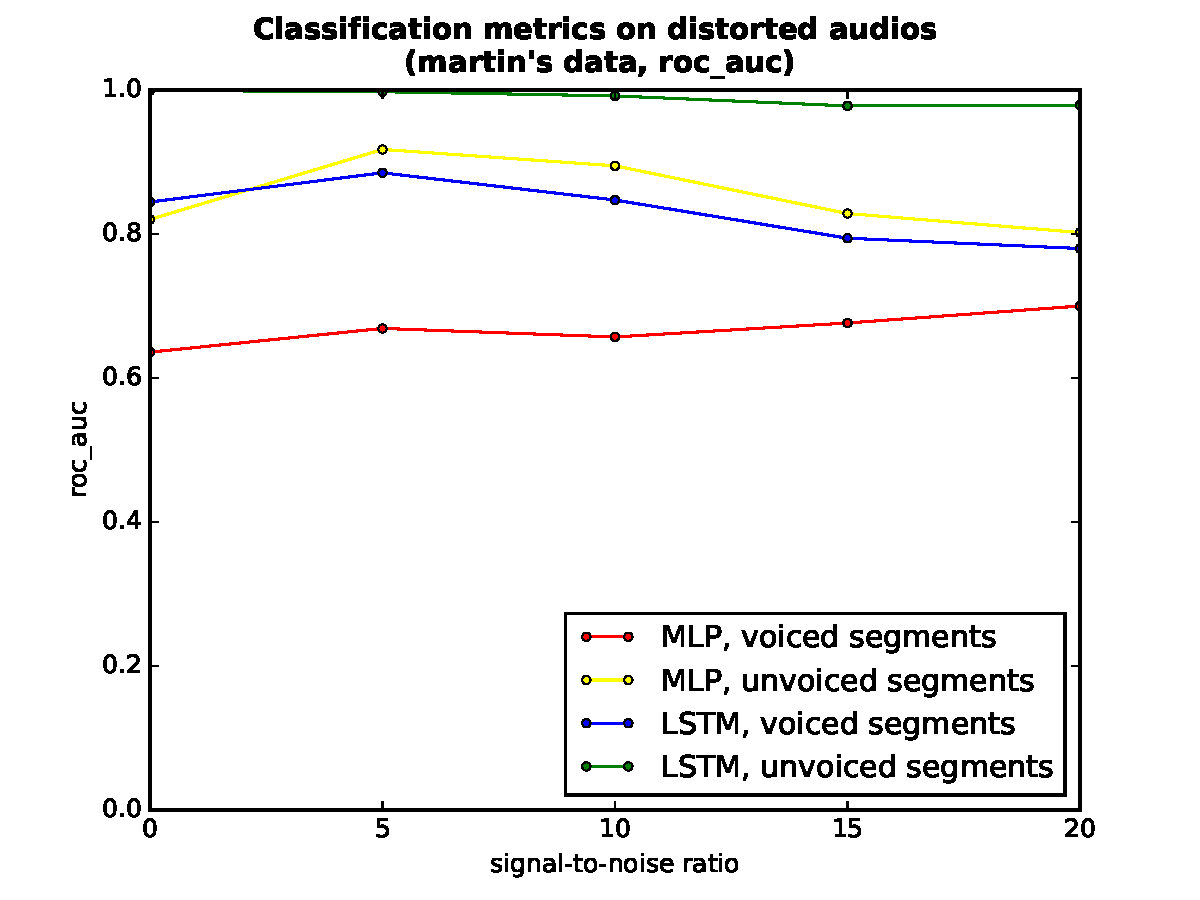
\includegraphics[width=0.65\textwidth]{classification_metrics_martin_roc_auc.pdf}
  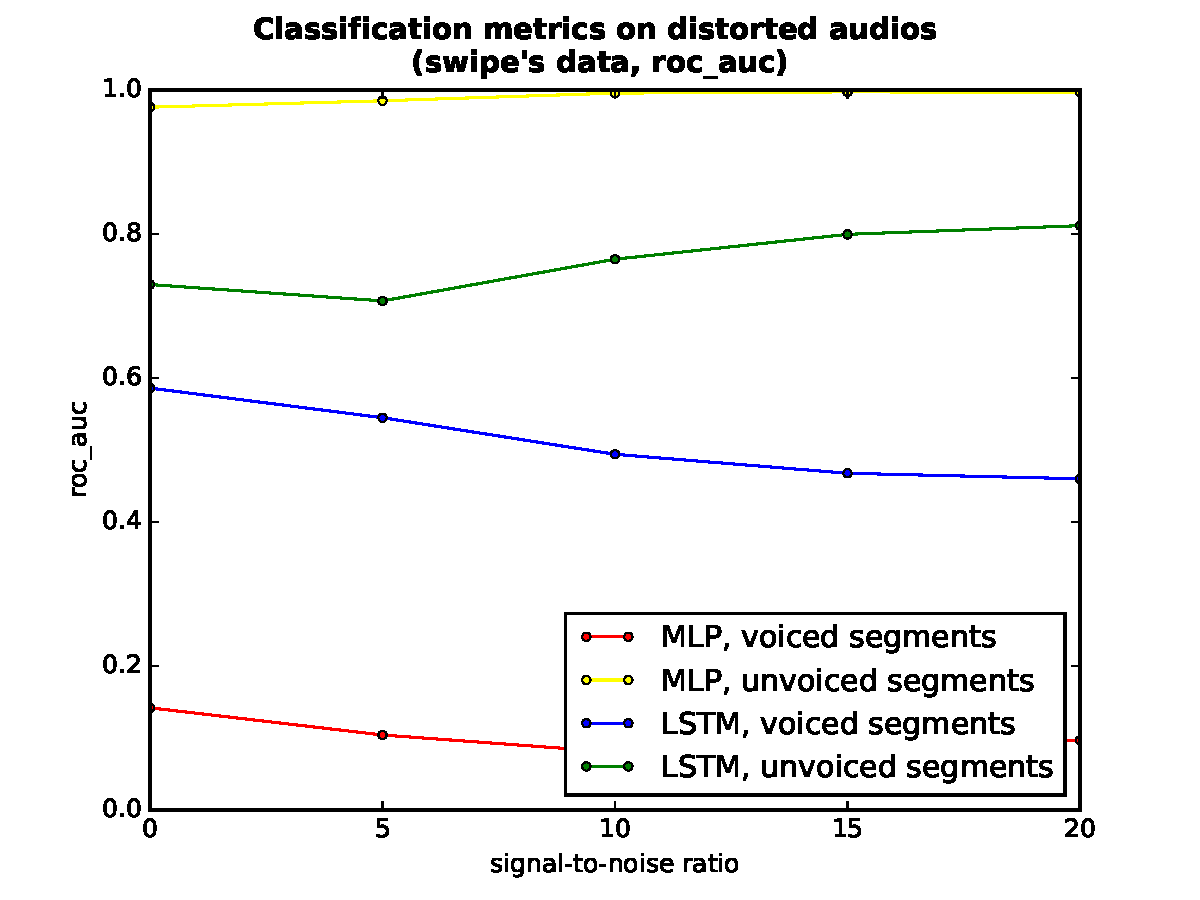
\includegraphics[width=0.65\textwidth]{classification_metrics_swipe_roc_auc.pdf}
  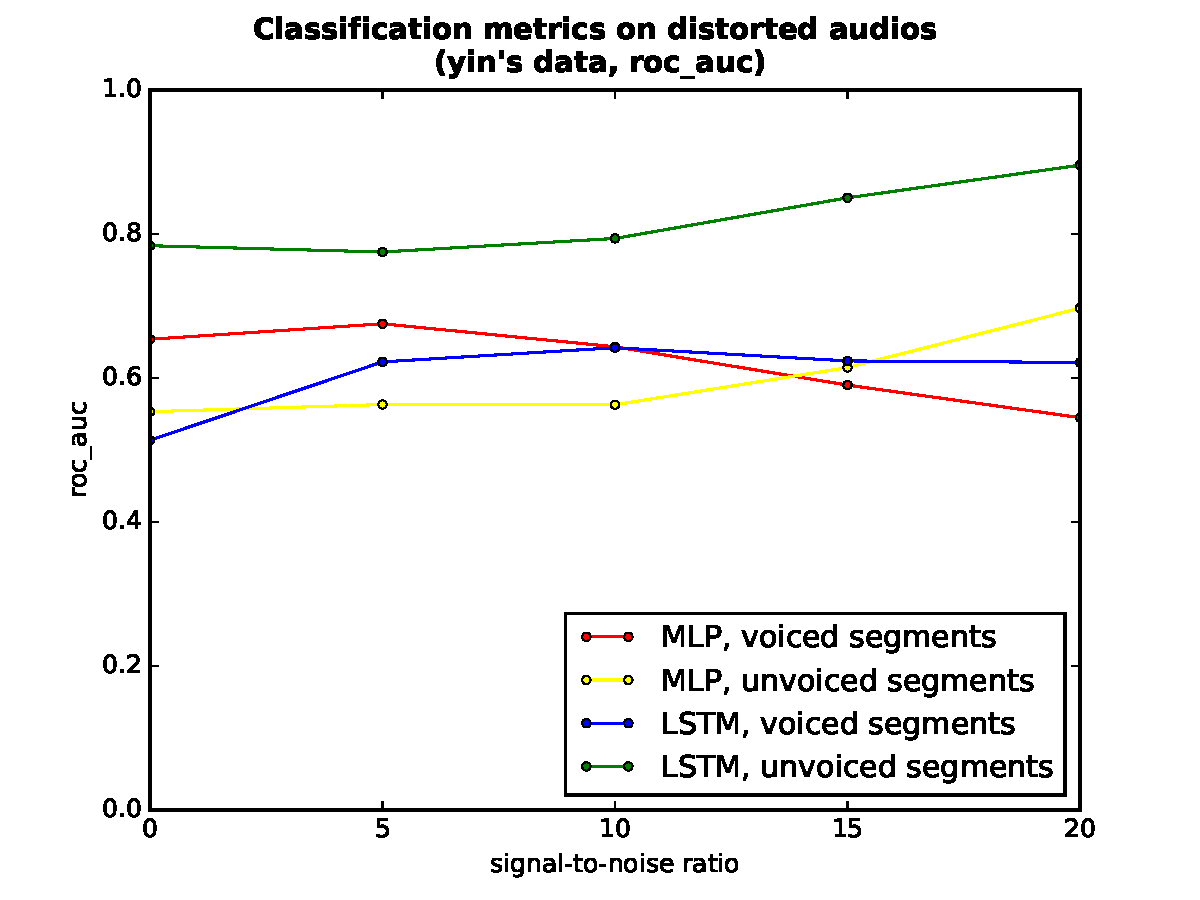
\includegraphics[width=0.65\textwidth]{classification_metrics_yin_roc_auc.pdf}
  \caption{MLP model and LSTM model's ROC AUCs on distorted testing audio signals}
  \label{fig:distorted-testing-data-roc-auc}
\end{figure}

\begin{figure}[htbp]
  \centering
  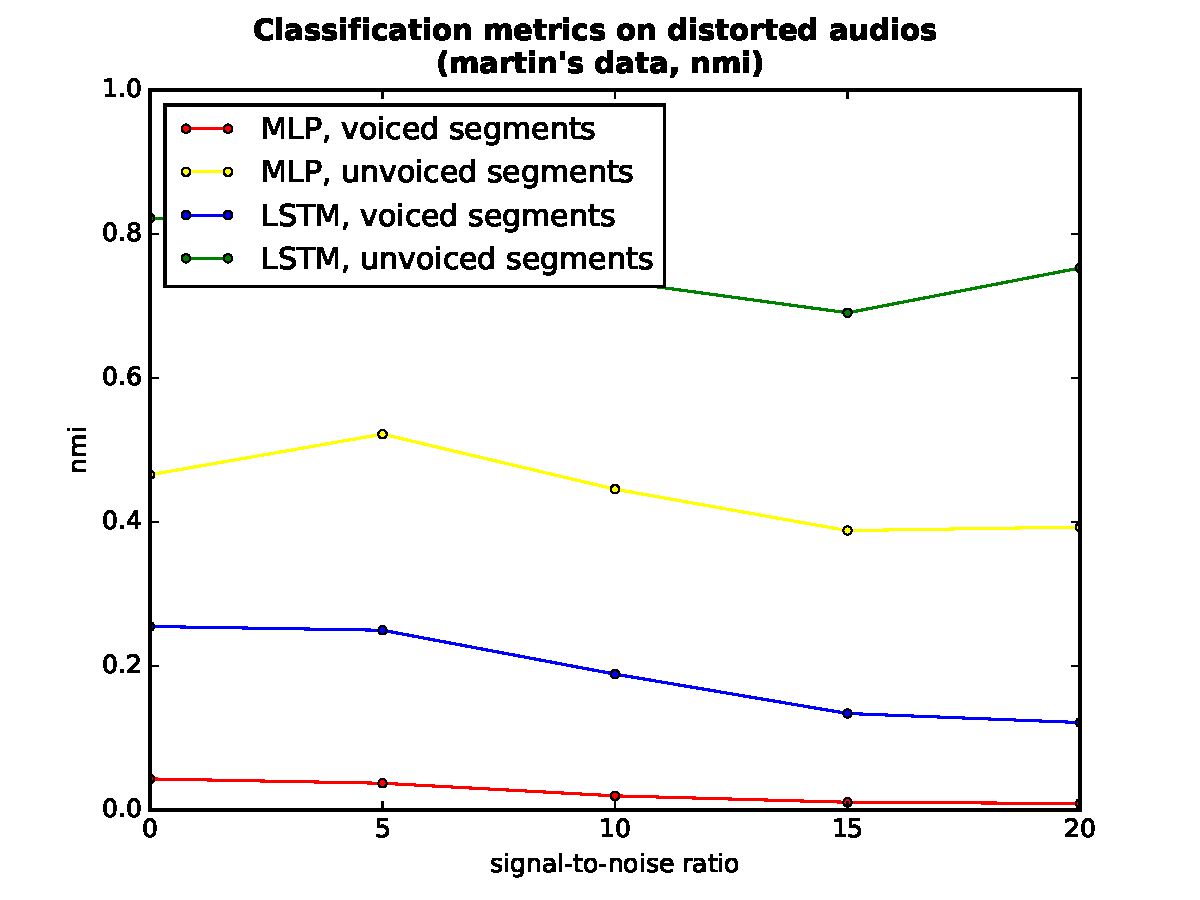
\includegraphics[width=0.65\textwidth]{classification_metrics_martin_nmi.pdf}
  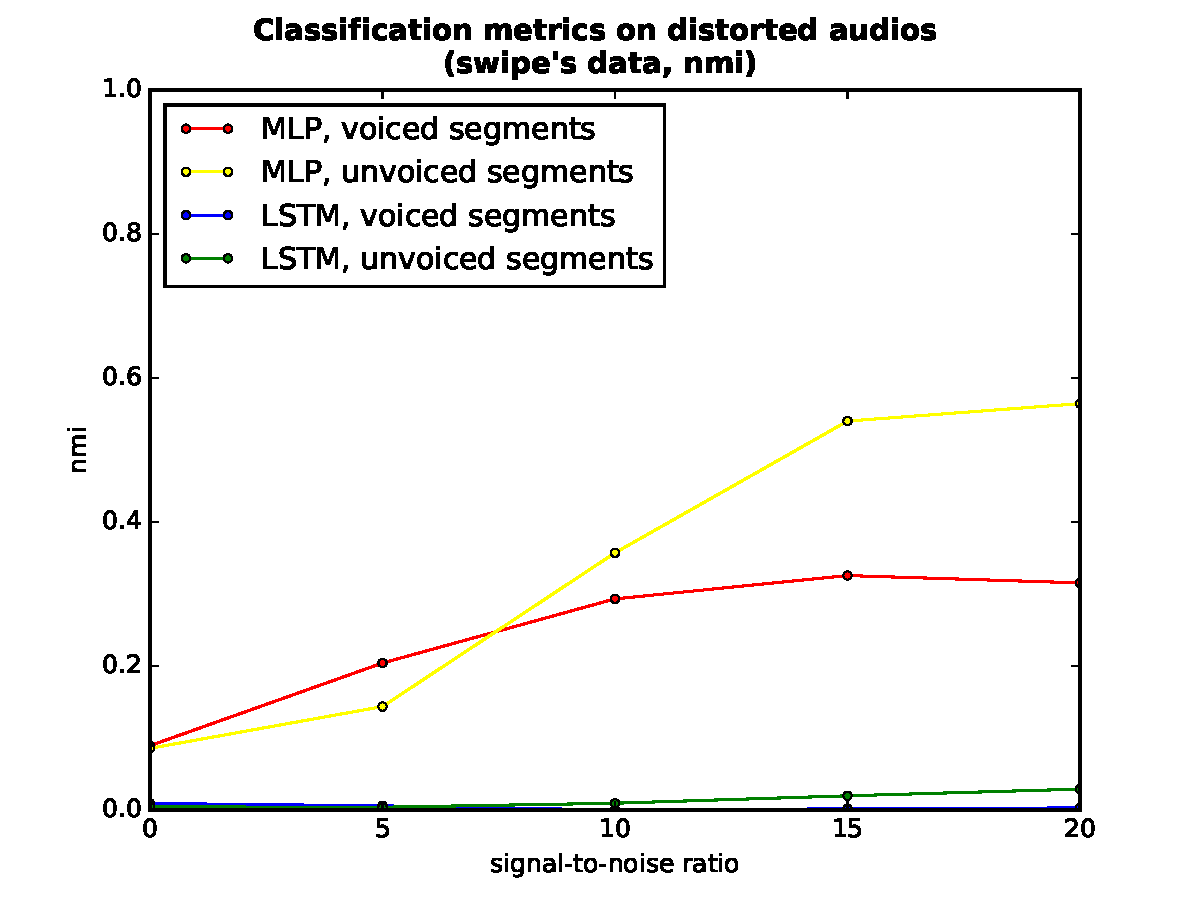
\includegraphics[width=0.65\textwidth]{classification_metrics_swipe_nmi.pdf}
  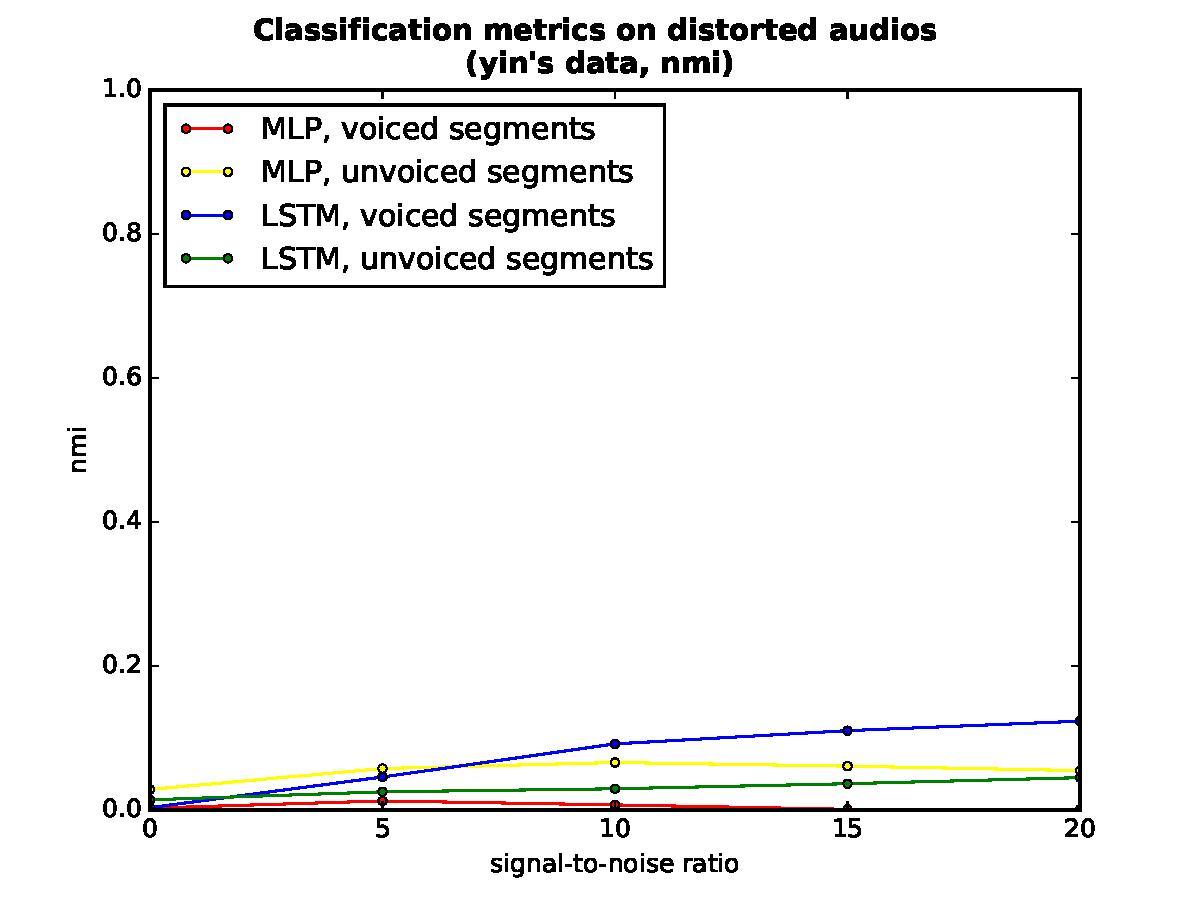
\includegraphics[width=0.65\textwidth]{classification_metrics_yin_nmi.pdf}
  \caption{MLP model and LSTM model's NMIs on distorted testing audio signals}
  \label{fig:distorted-testing-data--nmi}
\end{figure}

\chapter{Conclusion}

We are the first in this field to tackle the problem of designing confidence measures for fundamental frequency estimations.

Our outcome is a universally applicable yet customizable and extensible neural network-based framework able to output confidence values directly.
There is no need to modify the target fundamental frequency estimation algorithm, as long as the estimated frequencies and other features are involved in training.

Its excellent performance is demonstrated on several existing fundamental frequency estimation algorithms, which shows its utility value.

\section*{Future work}

\begin{itemize}
  \item Bidirectional LSTMs may work even better by also looking \enquote{forwards} in the sequences.
    It's reasonable to assume that there are temporal dependencies on future time steps.
  \item Neural network regression models are able to output an estimated frequency along with the confidence, like an ensemble method, and estimated frequencies from various algorithms can be used as features.
  \item We may further investigate the possibility of using a convolutional neural network (CNN) to calculate the fundamental frequency values, working directly on the spectrogram.
\end{itemize}

\appendix

\chapter{Appendix}

We use \texttt{pandas} \parencite{mckinney2010data} to do data preparation and \texttt{matplotlib} \parencite{hunter2007matplotlib} for plotting.
Neural networks are implemented using \texttt{Python} and \texttt{Keras} \parencite{chollet2015keras} library.

\bigskip

All the code used in this work is hosted at \url{https://github.com/bryandeng/f0-cm}, along with necessary documentation.

\bigskip

Some of the experiments are run on Grid'5000 \parencite{balouek2012adding}.

\printbibliography

\end{document}
